\documentclass[12pt,a4paper,bibliography=totocnumbered,listof=totoc]{scrartcl}
\usepackage[ngerman]{babel}
\usepackage[T1]{fontenc}% wichtig für Trennung von Wörtern mit Umlauten
\usepackage{microtype}% verbesserter Randausgleich
\usepackage[utf8]{inputenc}
\usepackage{amsmath}
\usepackage{amsfonts}
\usepackage{amssymb}
\usepackage{graphicx}
\usepackage{fancyhdr}
\usepackage{multirow, tabularx}
\usepackage{geometry}
\usepackage{setspace}
\usepackage[right]{eurosym}
\usepackage[printonlyused]{acronym}
\usepackage{subfig}
\usepackage{floatflt}
\usepackage[usenames,dvipsnames]{color}
\usepackage{colortbl}
\usepackage{paralist}
\usepackage{array}
\usepackage{titlesec}
\usepackage{parskip}
\usepackage[right]{eurosym}
\usepackage{picins}
\usepackage[subfigure,titles]{tocloft}
\usepackage[pdfpagelabels=true]{hyperref}
\usepackage{chngcntr}
\counterwithin{figure}{section}
\usepackage{natbib}
\bibliographystyle{dinat}

\usepackage{listings}
\lstset{basicstyle=\footnotesize, captionpos=b, breaklines=true, showstringspaces=false, tabsize=2, frame=lines, numbers=left, numberstyle=\tiny, xleftmargin=2em, framexleftmargin=2em}
\makeatletter
\def\l@lstlisting#1#2{\@dottedtocline{1}{0em}{1em}{\hspace{1,5em} Lst. #1}{#2}}
\makeatother

\geometry{a4paper, top=27mm, left=30mm, right=30mm, bottom=35mm, headsep=10mm, footskip=12mm}

\hypersetup{unicode=false, pdftoolbar=true, pdfmenubar=true, pdffitwindow=false, pdfstartview={FitH},
	pdftitle={Abschlussarbeit},
	pdfauthor={Philipp Anders},
	pdfsubject={Bachelorarbeit},
	pdfcreator={\LaTeX\ with package \flqq hyperref\frqq},
	pdfproducer={pdfTeX \the\pdftexversion.\pdftexrevision},
	pdfkeywords={Bachelorarebti},
	pdfnewwindow=true,
	colorlinks=true,linkcolor=black,citecolor=black,filecolor=magenta,urlcolor=black}
\pdfinfo{/CreationDate (D:20110620133321)}

\begin{document}

\titlespacing{\section}{0pt}{12pt plus 4pt minus 2pt}{-6pt plus 2pt minus 2pt}

% Kopf- und Fusszeile
\renewcommand{\sectionmark}[1]{\markright{#1}}
\renewcommand{\leftmark}{\rightmark}
\pagestyle{fancy}
\lhead{}
\chead{}
\rhead{\thesection\space\contentsname}
\lfoot{}
\cfoot{}
\rfoot{\thepage}
\renewcommand{\headrulewidth}{0.4pt}
% \renewcommand{\footrulewidth}{0.4pt}

% Vorspann
\renewcommand{\thechapter}{\Roman{chapter}}
\pagenumbering{Roman}
\raggedbottom

% ----------------------------------------------------------------------------------------------------------
% Titelseite
% ----------------------------------------------------------------------------------------------------------
\thispagestyle{empty}
\begin{center}
	\vspace*{1cm}
	\textbf{Hochschule für Technik, Wirtschaft und Kultur Leipzig}\\
	\vspace*{0.3cm}
	Fakultät Informatik, Mathematik und Naturwissenschaften\\
	Bachelorstudiengang Medieninformatik\\
	\vspace*{1cm}
	Bachelorarbeit\\
	zur Erlangung des akademischen Grades\\
	\vspace*{0.3cm}
	\textbf{Bachelor of Science (B.Sc.)}\\
	\Huge
	\vspace*{1cm}
	\textbf{Integration des Tacton Produktkonfigurators in ein Open Source Shopsystem}\\
	
	\vfill
	\normalsize
	\newcolumntype{x}[1]{>{\raggedleft\arraybackslash\hspace{0pt}}p{#1}}
	\begin{tabular}{x{3cm}p{10cm}}
		\rule{0mm}{5ex}\textbf{eingereicht von:} & Philipp Anders\newline Matrikelnummer: 58359 \\ 
		\rule{0mm}{5ex}\textbf{Betreuer:} & Prof. Dr. Michael Frank (HTWK Leipzig)\newline Dipl.-Wirt.-Inf. (FH) Dirk Noack (Lino GmbH)\\ 
		\rule{0mm}{5ex}\textbf{Abgabedatum:} & 28.09.2015 \\ 
	\end{tabular} 
\end{center}
\pagebreak

% ----------------------------------------------------------------------------------------------------------
% Abstract
% ----------------------------------------------------------------------------------------------------------
\setcounter{page}{1}
\onehalfspacing
\titlespacing{\section}{0pt}{12pt plus 4pt minus 2pt}{2pt plus 2pt minus 2pt}
\section*{Kurzfassung}
Das ganze auf Deutsch.

\vspace{-1,2em}
\titlespacing{\section}{0pt}{12pt plus 4pt minus 2pt}{-6pt plus 2pt minus 2pt}
\section*{Abstract}
Das ganze auf Englisch.
\pagebreak

% ----------------------------------------------------------------------------------------------------------
% Verzeichnisse
% ----------------------------------------------------------------------------------------------------------
% TODO Typ vor Nummer
\renewcommand{\cfttabpresnum}{Tab. }
\renewcommand{\cftfigpresnum}{Abb. }
\settowidth{\cfttabnumwidth}{Abb. 10\quad}
\settowidth{\cftfignumwidth}{Abb. 10\quad}

\rhead{Inhaltsverzeichnis}
\setcounter{secnumdepth}{3} 
\setcounter{tocdepth}{3}
\tableofcontents
\pagebreak
\rhead{Verzeichnisse}
\listoffigures
\pagebreak
\listoftables
\pagebreak
\renewcommand{\lstlistlistingname}{Listing-Verzeichnis}
\lstlistoflistings
\pagebreak

% ----------------------------------------------------------------------------------------------------------
% Abkürzungen
% ----------------------------------------------------------------------------------------------------------
\chapter*{Abkürzungsverzeichnis}
\addcontentsline{toc}{chapter}{Abkürzungsverzeichnis} 
\begin{acronym}[WSDL] % längste Abkürzung steht in eckigen Klammern
	\setlength{\itemsep}{-\parsep} % geringerer Zeilenabstand
	\acro{AJAX}{asynchronous JavaScript and XML}
	\acro{API}{Application Programming Interface}
	\acro{ATO}{Assemble-to-Order}
	\acro{B2B}{Business-to-Business}
	\acro{B2C}{Business-to-Customer}
	\acro{CORS}{Cross-Origin Resource Sharing}
	\acro{CSP}{Constraint Satisfaction Problem}
	\acro{etc.}{et cetera}
	\acro{ETO}{Engineer-to-Order}
	\acro{i.d.R.}{in der Regel}
	\acro{JSON}{JavaScript Object Notation}
	\acro{MC}{Mass Customization}
	\acro{MTO}{Make-to-Order}
	\acro{MVC}{Model View Controller}
	\acro{ORM}{objektrelationale Abbildung}
	\acro{PTO}{Pick-to-Order}
	\acro{RPC}{Remote Procedure Call}
	\acro{SOP}{Same-Origin-Policy}
	\acro{UML}{Unified Modeling Language}
	\acro{URI}{Uniform Resource Identifier}
	\acro{vgl.}{vergleiche}
	\acro{WSDL}{Web Service Description Language}
\end{acronym}
\newpage

% ----------------------------------------------------------------------------------------------------------
% Inhalt
% ----------------------------------------------------------------------------------------------------------
% Abstände Überschrift
\titlespacing{\section}{0pt}{12pt plus 4pt minus 2pt}{0pt plus 2pt minus 2pt}
\titlespacing{\subsection}{0pt}{12pt plus 4pt minus 2pt}{-1pt plus 2pt minus 2pt}
\titlespacing{\subsubsection}{0pt}{12pt plus 4pt minus 2pt}{-1pt plus 2pt minus 2pt}

% Kopfzeile
\renewcommand{\sectionmark}[1]{\markright{#1}}
\renewcommand{\subsectionmark}[1]{}
\renewcommand{\subsubsectionmark}[1]{}
\lhead{Kapitel \thesection}
\rhead{\rightmark}

\onehalfspacing
\renewcommand{\thesection}{\arabic{section}}
\renewcommand{\theHsection}{\arabic{section}}
\setcounter{section}{0}
\pagenumbering{arabic}
\setcounter{page}{1}


\section{Einleitung}

\subsection{Ziel der Arbeit}

\subsection{Aufbau der Arbeit}

\pagebreak

\section{Grundlagen}

\subsection{Bezugsrahmen}
Im Folgenden wird ein Bezugsrahmen für Produktkonfigurationssysteme (Konfiguratoren) geschaffen. Dazu wird zunächst die marktwirtschaftliche Situation erläutert, welche die Notwendigkeit hybrider Wettbewerbsstrategien begründet. Diese wiederum stellen zu ihrer Umsetzbarkeit Bedingungen an Produktionskonzepte, welche daraufhin vorgestellt werden.

\subsubsection{Ökonomischer Bezug}
\label{subsubsection:oekonomischerBezug}
Neue Wettbewerbsbedingungen und gesteigerte Kundenansprüche haben den Druck auf Industrieunternehmen zur Produktion individualisierter Produkte erhöht \citep{piller98}. Dies erfordert eine stärkere Leistungsdifferenzierung \citep{lutz11}. Diese ist eine der von \citeauthor{porter02} beschriebenen \glqq generischen Wettbewerbsstrategien\grqq{}. Sie entspricht dem Verkauf von Produkten mit höherem individuellen Kundennutzen zu höheren Preisen. Eine andere Wettbewerbsstrategie ist die  Fokussierungsstrategie. Diese bezieht sich klassischerweise auf Anbieter von Massenproduktion. Durch die Unterbietung der Konkurrenzpreise wird der Marktanteil erhöht. 

\vspace{1em}
\begin{minipage}{\linewidth}
	\centering
	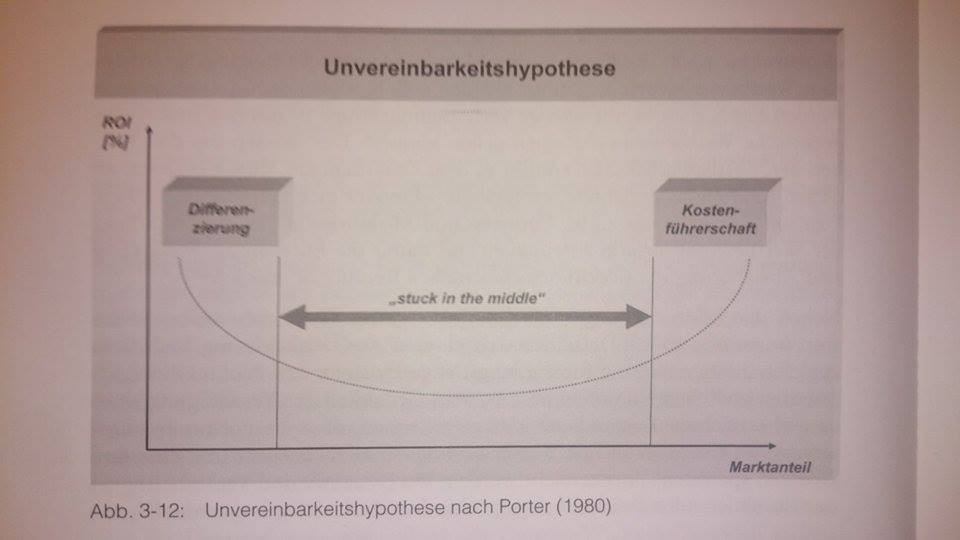
\includegraphics[width=0.7\linewidth]{Abbildungen/unvereinbarkeitshypothese.jpg}
	\captionof{figure}[Unvereinbarkeitshypothese]{Unvereinbarkeitshypothese nach \cite{porter80}, zitiert von \cite{schuh05}}
	\label{fig:unvereinbarkeitshypothese}
\end{minipage}
\vspace{1em}

In diesem Zusammenhang formulierte \citeauthor{porter80} die Unvereinbarkeitshypothese. So sollen Kostenführerschaft und Leistungsdifferenzierung nicht gleichzeitig erreichbar sein. Eine uneindeutige Positionierung führe zu einem \glqq stuck in the middle\grqq{} und damit zur Unwirtschaftlichkeit, wie Abbildung \ref{fig:unvereinbarkeitshypothese} darstellt.

Die Beobachtung der Unternehmensrealität zeichnet ein anderes Bild. Neue Organisatzionsprinzipien, Informationsverarbeitungspotentiale und Produktstrukturierungsansätze ermöglichen einen Kompromiss aus Preis- und Leistungsführerschaft \citep{schuh05}. Das Ergebnis wird als hybride Wettbewerbsstrategien bezeichnet. Eine dieser Strategien ist die sogenannte \ac{MC}.

\ac{MC} ist die \glqq Produktion von Gütern und Leistungen für einen (relativ) großen Absatzmarkt, welche die unterschiedlichen Bedürfnisse jedes einzelnen Nachfragers dieser Produkte treffen, zu Kosten, die ungefähr denen einer massenhaften Fertigung vergleichbarer Standardgüter entsprechen\grqq{} \citep{piller98}. Mit anderen Worten: Preisvorteil (i.d.R. durch Massenfertigung) wird mit Individualisierung (i.d.R. durch Variantenvielfalt) vereint.

\subsubsection{Produktklassifizierung}
 \label{subssubsection:Produktklassifizierung}

\ac{MC} stellt zu deren Umsetzbarkeit gewisse Bedingungen an die Produktionsweisen der abzusetzenden Güter. Im Folgenden wird eine Klassifizierung von Produkten in Bezug zu deren Herstellung vorgestellt. Die Typen werden als Produktionskonzepte bezeichnet  (nach \citealt{schuh06}, zitiert von \citealt{lutz11}):
\begin{compactitem}
	\item \textbf{\ac{PTO}:} Herstellung ohne Kundenauftrag; Lagerhaltung auf Ebene ganzer Produkte; Keine Abhängigkeit dieser Produkte untereinander;\\
	Beispiel: Ein Standardnotebook.
	\item \textbf{\ac{ATO}:} Herstellung ohne Kundeauftrag; Lagerhaltung auf Ebene der Baugruppen/-teilen; Teile mit Abhängigkeiten untereinander;\\
	Beispiel: Ein Notebook, bei welchem auf Kundenwunsch statt des CD-Laufwerks eine zusätzliche Festplatte eingebaut wird. Die Festplatte wurde bereits im Lager vorgehalten.
	\item \textbf{\ac{MTO}:} Herstellung teilweise erst nach Kundenenauftrag; Lagerhaltung auf Ebene der Baugruppen/-teilen; Produktion oder regelbasierte (parametrisierte) Konstruktion von Komponenten nach Kundenanforderung; Abhängigkeiten zwischen Teilen; keine unendliche Anzahl von Varianten;\\
		Beispiel: Kauf eines Notebooks, wobei der Kunde eine Displaygröße abweichend von den Standarddiagonallängen bestimmen kann. Display und Notebookgehäuse müssen konstruiert/hergestellt und die technischen Standardkomponenten (z.B. Festplatte, Motherboard) eingepasst werden. 
	\item \textbf{\ac{ETO}:} Produkt ist nicht komplett vom Hersteller vorhersehbar; Wenig bis keine Lagerhaltung auf Ebene der Baugruppen/-teilen; Entwicklung und Fertigung von Teilen nach Kundenspezifikation; unendliche Variantenanzahl möglich;\\
	Beispiel: Herstellung eines Notebooks mit Kaffeetassenhalterung.
\end{compactitem}

Die Produktionskonzepte unterscheiden sich hauptsächlich danach, wann die Produktion der Baugruppen/-teile beginnt -- ob vor oder nach Auftragsspezifikation. Eine Produktion vor Auftragseingang, also ohne Kundenspezifikation, erlaubt Lagerhaltung. Ein hoher Komponentenanteil, der erst nach Auftragseingang hergestellt oder sogar konstruiert werden muss, spricht für eine starke Kundenindividualisierung \citep{lutz11}. Die unterschiedlichen Produktionskonzepte haben jeweils einen Anwendungsbezug zu Konfiguratoren, welche im Folgenden vorgestellt werden.

\pagebreak
\subsection{Produktkonfiguration}
\label{subssubsection:Produktkonfiguration}
 
Aus der im vorangegangenen Kapitel vorgestellten \ac{MC} resultiert mehr Produktvariabilität und damit Produktkomplexität. Die Produktkonfiguration (Konfiguration) ist ein Werkzeug zur Beherrschung dieser Komplexität. Sie unterstützt das Finden einer Produktvariante, die auf Kundenanforderungen angepasst und gleichzeitig machbar ist \citep{lutz11}.

\subsubsection{Begriffsüberblick}
\label{subsubsection:begriffsuberblick}
\textbf{Konfiguration} ist eine spezielle Designaktivität, bei der der zu konfigurierende Gegenstand aus Instanzen einer festen Menge wohldefinierter Komponententypen zusammengesetzt wird, welche entsprechend einer Menge von Konfigurationsregeln (Constraints) kombiniert werden können \citep{sabin98}.

Die Einordnung als Designaktivität erlaubt außerdem die Beschreibung der Konfiguration als ein Designtyp. Es werden das \glqq Routine Design\grqq{}, \glqq Innovative Design\grqq{} und \glqq Creative Design\grqq{} unterschieden. Die Konfiguration entspricht dem \glqq Routine Design\grqq{}. Dabei handelt es sich um ein Problem, bei der die Spezifikation der Objekte, deren Eigenschaften sowie kompositionelle Struktur vorgegeben ist und die Lösung auf Basis einer bekannten Strategie gefunden wird \citep{brown89}. Damit ist \glqq Routine Design\grqq{} die simpelste der drei Formen. Die anderen Designtypen enthalten hingegen Objekte und Objektbeziehungen, die erst während des Designprozesses entwickelt werden.

Die Schlüsselbegriffe der Definition von \citeauthor{sabin98} sind Komponententypen und Constraints. \textbf{Komponententypen} sind Kombinationselemente, welche durch Attribute charakterisiert werden und eine Menge alternativer (konkreter) Instanzen repräsentieren. Übertragen auf die objektorientierte Programmierung verhalten sich Komponententypen zu Instanzen wie Klassen zu Objekten. Komponententypen stehen zueinander in Beziehung. Diese kann entweder eine \glqq Teil-Ganzes\grqq{}-Beziehung oder Generalisierung sein \citep{felferning14}. 

\textbf{Constraints} (d.h. Konfigurationsregeln) im engeren Sinne sind Kombinationseinschränkungen \citep{felferning14}. Weitere Arten werden später vorgestellt.

Zur besseren Nachvollziehbarkeit der weiteren Terminologie ist eine Definition des Variantenbegriffs angebracht. DIN 199 beschreibt Varianten als \glqq Gegenstände ähnlicher Form und/oder Funktion mit einem in der Regel hohen Anteil identischer Gruppen oder Teile\grqq{}. Varianten sind also Gegenstandsmengen. Eine Element dieser Menge unterscheidet sich von einer anderen durch mindestens eine Beziehung oder ein Element \citep{lutz11}.

Die Einheit aus Komponententypen sowie das Wissen um deren Kombinierbarkeit in Form von Constraints wird als \textbf{Konfigurationsmodell} bezeichnet. Es bildet die Menge der korrekten Lösungen ab und definiert so implizit alle Varianten eines Produktes \citep{soininen98}. Dadurch muss nicht jede Variante explizit definiert und abgespeichert werden (z.B. in einer Datenbank). Die Anzahl möglicher Kombinationen kann in die Millionen gehen, was die Suche nach einer bestimmten sehr zeitaufwändig machen würde \citep{falkner11}.

Die Einheit aus Konfigurationsmodell und den Kundenanforderungen wird als \textbf{Konfigurationsaufgabe} bezeichnet \citep{felferning14}. Auf deren Grundlage kann die gewünschte Konfiguration errechnet werden. Demzufolge ist der Begriff Konfiguration überladen: er bezeichnet sowohl den technischen Prozess der Lösungsfindung als auch die Lösung selbst. Im Folgenden werden daher die Begriffe \textbf{Konfigurationsprozess} sowie \textbf{Konfigurationslösung} verwendet. Der Konfigurationsprozess wird von einem System durchgeführt. Dieses wird als \textbf{Konfigurator} bezeichnet.

Diese Beschreibung einer Konfigurationslösung suggeriert, dass zu Beginn des Konfigurationsprozesses einmalig die Konfigurationsaufgabe formuliert und daraufhin die Konfigurationslösung ermittelt wird. Diese Form wird als \textbf{statische Konfiguration} bezeichnet. Demgegenüber erlaubt die \textbf{interaktive Konfiguration} das schrittweise Treffen und Revidieren von Entscheidungen \citep{hadzic04}. Die Menge aller bisher getroffenen Entscheidungen wird als \textbf{Konfigurationszustand} bezeichnet \citep{tactonTCsiteDevelopmentManual}. Der Konfigurator muss beim Konfigurationsprozess einen Mechanismus besitzen, der die Konfigurationsaufgabe in Bezug mit dem Konfigurationszustand bringt.

\subsubsection{Wissensrepräsentation}
\label{subsubsection:wissenrepraesentation}
Das Konfigurationswissen beschreibt Wissen, welches über ein konfigurierbares Produkt besteht \citep{soininen98}. Dieses Wissen kann auf unterschiedliche Art und Weise repräsentiert, d.h. dargestellt werden. Die Repräsentation kann zur Definition eines Konfigurationsmodells genutzt werden \citep{felferning14}. Auf konzeptioneller Ebene werden die Begriffe Wissensrepräsentation und Konfigurationsmodell äquivalent verwendet. Auf technischer Ebene bezeichnet das Konfigurationsmodell jedoch das spezifische Format, welches ein Konfigurator versteht \citep{soininen98}.

Im Folgenden wird ein grafische Wissensrepräsentation vorgestellt, die auf UML basiert. Die grafische Variante wird gewählt, da sie die Bildung einer Vorstellung über die Problemdomäne zulässt. Sie ist UML-basiert, da die Sprache in der Informatik zur Wissensmodellierung bekannt ist. Im Folgenden wird eine Notebook-Konfiguration eingeführt und von späteren Erklärungen wieder aufgegriffen. Die Modellierung basiert auf dem Arbeitsbeispiel von \citep{felferning14}.

\vspace{1em}
\begin{minipage}{\linewidth}
	\centering
	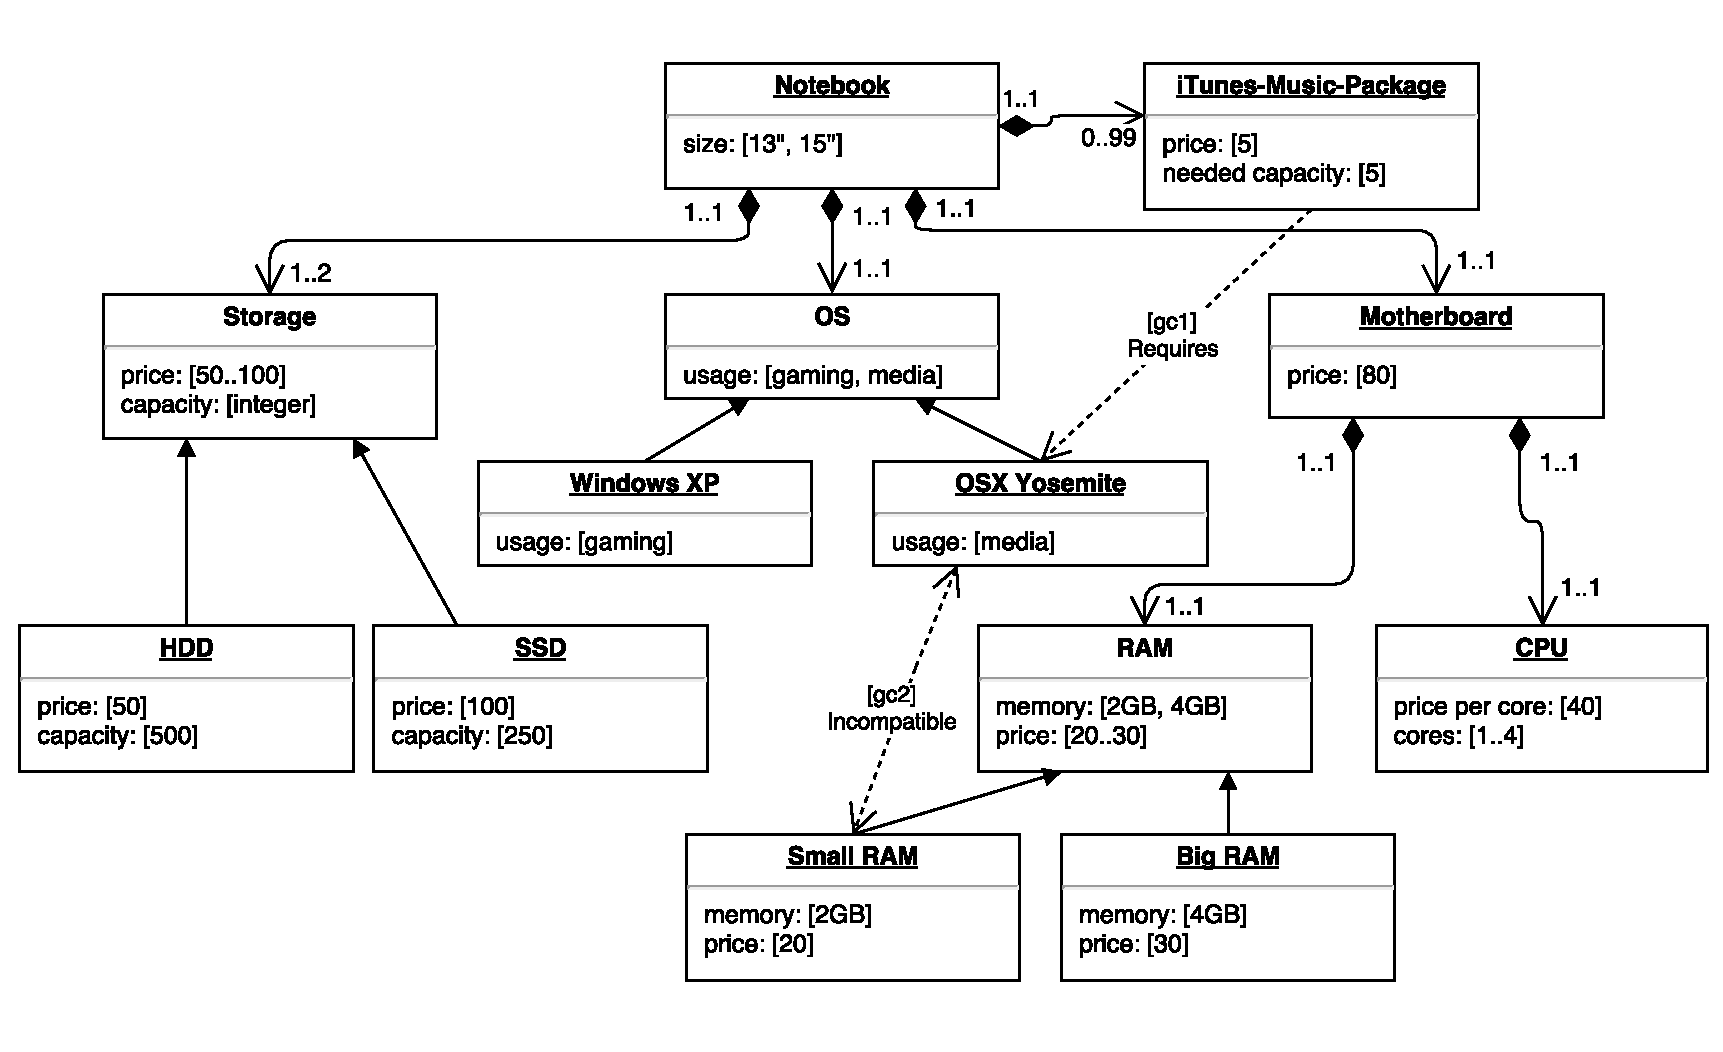
\includegraphics[width=1\linewidth]{Abbildungen/notebookConfigurationUML.pdf}
	\captionof{figure}[notebookConfigurationUML]{UML-Visualisierung einer Notebook-Konfiguration\footnote{Das 'iTunes-Music-Package' stellt ein Überraschungspaket mit Musik für iTunes dar.}}
	\label{fig:notebookConfigurationUML}
\end{minipage}
\vspace{1em}

\begin{table}[]
\centering
\caption{Constraints des Konfigurationsmodells aus Abbildung \ref{fig:notebookConfigurationUML}}
\label{tab:notebookConfigurationConstraints}
\begin{tabularx}{\textwidth}{|l|X|}
\hline
{\bf Name} & {\bf Beschreibung}\\
\hline
$GC_1$ & Wird das \textbf{iTunes-Music-Package} gewählt, muss auch das Betriebssystem (OS) vom Typ\textbf{OSX Yosemite} gewählt werden. \\
\hline
$GC_2$ & Das OS vom Typ \textbf{OSX Yosemite} und der Arbeitsspeicher (RAM) vom Typ \textbf{Small RAM} können nicht gleichzeitig gewählt werden\\
\hline
$PRC_1$ & Der Preis des Notebooks ist die Summe der \textbf{price}-Attribute der Storage-, Motherboard-, RAM-, CPU- und iTunes-Music-Package-Komponenten\\
\hline
$RESC_1$ & Die Summe der \textbf{needed capacity}-Attribute aller iTunes-Music-Package-Komponenten darf die Summe der \textbf{capacity}-Attribute aller Storage-Komponenten nicht überschreiten\\
\hline
$CRC_1$ & Das OS vom Typ \textbf{OSX Yosemite} benötigt mindestens einen \textbf{core}-Wert der CPU-Komponente von 2\\
\hline
$COMPC_1$ & Das OS vom Typ \textbf{Windows XP} ist inkompatibel mit dem \textbf{size}-Wert des Notebooks von 13"\\
\hline
\end{tabularx}
\end{table}

Abbildung \ref{fig:notebookConfigurationUML} beschreibt den Strukturteil der Visualisierung. Folgende Sprachelemente sind enthalten \citep{felferning14}:
\begin{compactitem}
\item \textbf{Komponententypen} sind die dargestellten Entitäten. Sie besitzen einen eindeutigen Namen (z.B. 'Storage') und werden durch eine Menge von Attributen beschrieben (z.B. 'price', 'capacity'). Ein Attribute hat einen Datentyp, welcher eine Konstante, ein Wertebereich (z.B. [50...100]) oder eine Enumeration (z.B. ['gaming', 'media']) sein kann. Ein Komponententyp beschreibt ein abstraktes Konzept eines Bauteils. Beispielsweise ist ein 'CPU' etwas, was ein bis vier Kerne haben kann. Werden Attributewerte eines Komponententypen fest gewählt, wird daraus eine Instanz, d.h. ein konkretes Bauteil (z.B. ein Vierkernprozessor).
\item \textbf{Generalisierungen} stellen die Verbindungen zwischen einem spezialisierten Subtyp zu einem einem generalisierten Supertyp her. Damit muss der Wertebereich eines Attributs eines Subtypen eine Teilmenge des entsprechenden Attributwertebereichs des Supertypen sein. Komponententypen (z.B. 'Storage') werden so weiter spezialisiert (z.B. 'HD‘). Die Beziehung ist disjunkt und vollständig. Disjunkt bedeutet, dass jede Instanz eines Komponententypen nur genau einer seiner Subtypen entsprechen kann. Beispiel: Die Instanz eines 'Storage' kann eine 'HD' oder eine 'SSD' sein, aber nicht beides. Vollständig bedeutet, dass die Subtypen alle tatsächlich möglichen Instanzen darstellen (z.B. gibt es für diese Konfiguration keine Komponente 'DVD' als möglichen Storage).
\item \textbf{Assoziationen mit Kardinalitäten} beschreiben die Teil-Ganzes-Beziehungen zwischen Komponententypen. Die hier verwendete Variante ist die Komposition. Das bedeutet, dass keine Instanz eines Komponententypen Teil von mehr als einer anderen Instanz sein kann. Kardinalitäten beschreiben Assoziationen noch näher, indem sie sie durch Mengeninformationen ergänzen. Beispiel: Eine Notebook-Instanz besitzt ein oder zwei Storage-Instanzen. Eine Storage-Instanz kann nur Teil einer Notebook-Instanz sein.
\end{compactitem}

Die Darstellung wird ergänzt durch Constraints. Sie gelten zwischen Komponententypen und/oder deren Attributen. Wenn möglich werden sie direkt im Diagramm dargestellt. Anderenfalls werden sie in einer Tabelle aufgelistet (siehe Tabelle \ref{tab:notebookConfigurationConstraints}). Es werden folgende Constrainttypen unterschieden \citep{felferning14}:

\begin{compactitem}
\item \textbf{Grafische Constraints $GC$} können im Gegensatz zu anderen Constraints direkt im UML-Diagramm dargestellt werden. Ansonsten entsprechen sie einem der folgenden Typen.
\item \textbf{Preis-Constraints $PRC$} beziehen sich auf die Preisbildung der Konfiguration. Bei realer Konfigurationssoftware sind diese jedoch meistens nicht Teil des Konfigurationsmodells. Stattdessen wird die Preisbildung durch einen eigenen Mechanismus realisiert.
\item \textbf{Ressourcen-Constraints $RESC$} beschränken die Produktion und den Verbrauch bestimmter Ressourcen. Beispiel:  Jedes 'iTunes-Music-Package' verbraucht 5(MB) Festplattenkapazität. Der verfügbare Speicher wird wiederum durch die Storage-Instanzen bestimmt. Wird nur ein Speichermedium in Form einer 'SSD' gewählt, hat das Notebook 250(MB) Festplattenkapazität. Somit die Obergrenze für 'iTunes-Music-Package' Instanzen gleich 50.
\item \textbf{Abhängigkeits-Constraints $CRC$} beschreiben, unter welchen Voraussetzungen bestimmte Instanzen Teil der Konfigurationslösung sein müssen.
\item \textbf{Kompatibilitäts-Constraints $COMPC$:} Beschreiben die Kompatibilität  oder Inkompatibilität bestimmter Komponententypen bzw. Instanzen.
\end{compactitem}

\subsubsection{Konfigurationsaufgabe}
\citet{mittal89} definieren einen Konfigurationsaufgabe wie folgt:
\begin{quote}
(A) a fixed, pre-defined set of components, where a component is described by a set of properties, ports for connecting it to other components, constraints at each port that describe the components that can be connected at that port, and other structural constraints; (B) some description of the desired configuration; and (C) possibly some criteria for making optimal selections.
\end{quote}
(A) ist eine andere Definition für ein Konfigurationsmodell. (B) und (C) sind als Kundenanforderungen zusammenfassbar. Informell entsteht so die im Begriffsüberblick vorgestellte Definition: Die Konfigurationsaufgabe besteht aus dem Konfigurationsmodell sowie den Kundenanforderungen \citep{felferning14}.

\subsubsection{Konfigurationslösung}
\label{subsubsection:Konfigurationslösung}
Die Lösung einer Konfigurationsaufgabe ist vollständig (Jeder Komponententyp ist instanziiert) und konsistent (erfüllt alle Constraints) \citep[angelehnt an][]{falkner11}. Eine solche Lösung wird als korrekt bezeichnet \citep{soininen98}.

Eine korrekte Lösung kann durch ein UML-Instanz-Diagramm visualisiert werden.  Abbildung \ref{fig:notebookInstanceUML} zeigt eine korrekte Lösung der Notebook-Konfiguration. Dargestellt wird also eine mögliche Variante. Anstatt der Komponententypen sind nur noch konkrete Instanzen enthalten.

\vspace{1em}
\begin{minipage}{\linewidth}
	\centering
	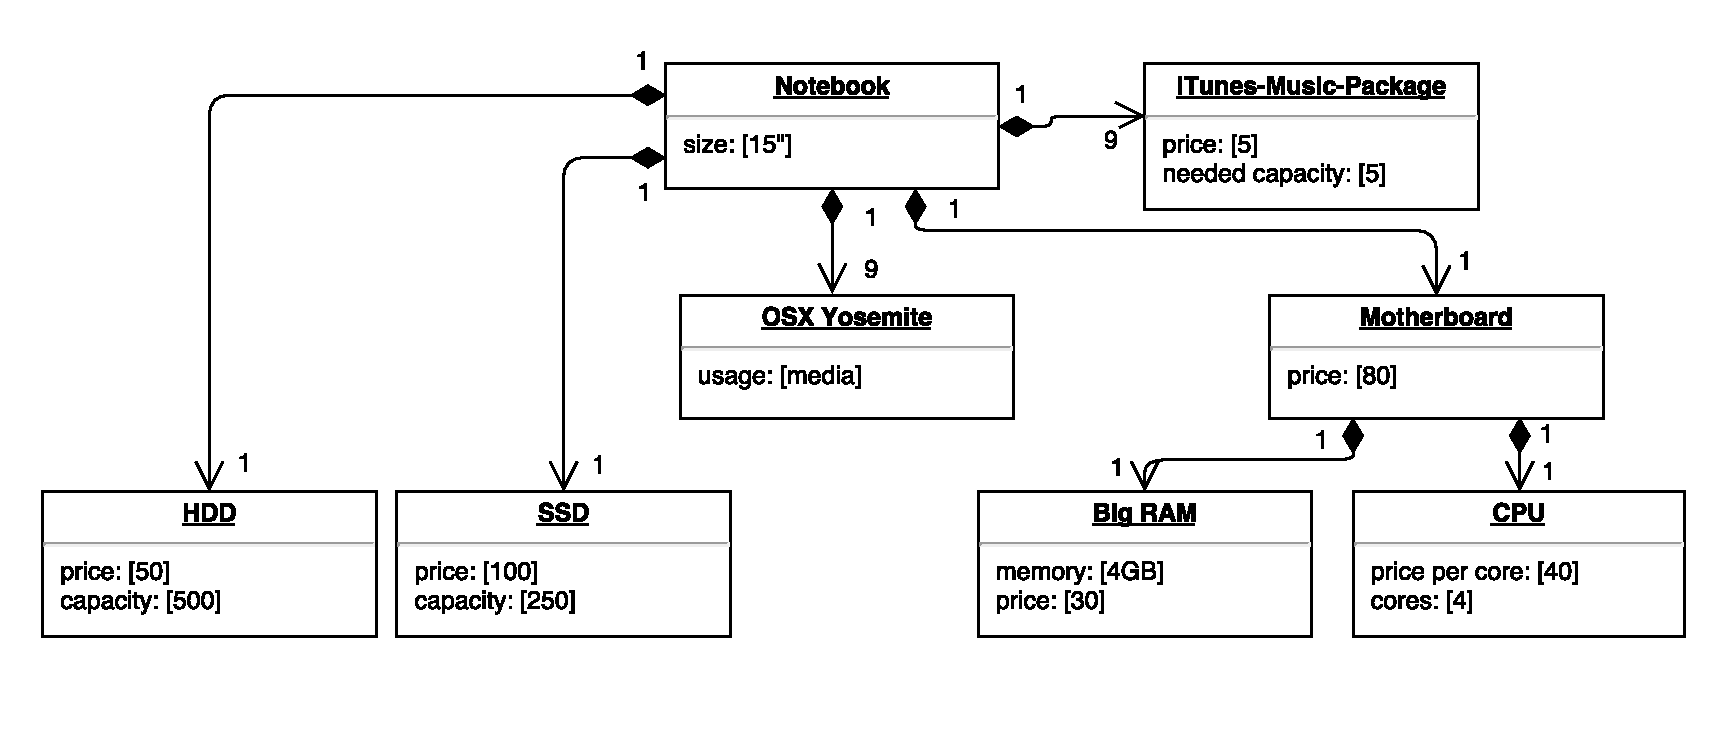
\includegraphics[width=1\linewidth]{Abbildungen/notebookInstanceUML.pdf}
	\captionof{figure}[notebookInstanceUML]{Visualisierung einer Konfigurationslösung als UML-Instanz-Diagramm}
	\label{fig:notebookInstanceUML}
\end{minipage}
\vspace{1em}

\subsubsection{Konfiguratoren}
\label{subsubsection:Konfigurationssysteme}
Konfiguratoren "[...] führen den Abnehmer durch alle Abstimmungsprozesse, die zur Definition des individuellen Produktes nötig sind und prüfen sogleich die Konsistenz sowie Fertigungsfähigkeit der gewünschten Variante" \citep{piller06}. Im Kapitel \ref{subsubsection:begriffsuberblick} wurde der Konfigurator hingegen als das System bestimmt, das den Konfigurationsprozess durchführt. Somit liegt erneut eine Begriffsüberladung vor. Aus technischer Sicht ist der Konfigurationsprozess der Vorgang der Verarbeitung einer Konfigurationsaufgabe. Aus Anwendersicht bezeichnet er den Abstimmungsprozess. Beides gehört zum Verantwortungsbereich des Konfigurators. Es wird im Folgenden die Konvention verwendet, dass der Begriff \glqq Konfigurationsprozess\grqq{} die Benutzerführung meint, der \glqq technische Konfigurationsprozess\grqq{} die Verarbeitung.

Nach \citet{piller06} besitzt ein Konfigurator drei Komponenten:
\begin{compactitem}
\item Die \textbf{Konfigurationskomponente} führt den technischen Konfigurationsprozess durch. Sie wird auch als Konfigurationsengine bezeichnet \citep{tactonProductOverview}.
\item Die \textbf{Präsentationskomponente} erstellt eine Konfigurationsdarstellung in zielgruppenspezifischer Form. Sie stellt die Schnittstelle für die Abstimmungsprozesse mit dem Anwender dar.
\item Die \textbf{Auswertungskomponente} präsentiert die Konfigurationslösung in einer Form, welche eine Interpretation der Variante außerhalb des Konfigurators erlaubt. Dies können zum Beispiel Stücklisten, Konstruktionszeichnungen und Arbeitspläne sein.
\end{compactitem}

\textbf{Konfiguratorarten}\\
Konfiguratoren für die Erhebung komplexer Anforderungen technischer Systeme  müssen von Konfiguratoren für den Einsatz bei \ac{MC} unterschieden werden \citep{felferning14}. Erstere sind für den Experteneinsatz gedacht oder dienen nach \citet{piller06} als Vertriebskonfiguratoren der Unterstützung des Verkaufsgespräches.   Letztere werden von Kunden in einer Company-to–Customer Beziehung genutzt und werden auch als Mass Customization Toolkit bezeichnet. Diese sogenannte Selbstkonfiguration ist eine Vorraussetzung für \ac{MC}, indem der zeitkonsumierende Prozess der Erhebung der Kundenbedürfnisse auf die Seite des Kunden verlagert wird \citep{piller06}

Konfiguratoren können bei allen in Abschnit \ref{subssubsection:Produktklassifizierung} genannten Produktionskonzepten zum Einsatz kommen. Je nach Produktionskonzept erfüllt der Konfigurationsprozess eine unterschiedliche Bedeutung. Bei \ac{PTO} hat der Konfigurator eine Katalogfunktion, indem er den Anwender bei der Auswahl eines fertigen Produktes aus einer Produktpalette unterstützt. Bei \ac{ATO} verhält sich der Konfigurator wie ein Variantengenerator, der den Anwender bei der Auswahl der richtigen Variante unterstützt. Wohlgemerkt: der Hersteller hat alle möglichen Varianten vordefiniert, sie sind also herstellerspezifisch \citep{schomburg80}. Der Anwendungsfall \ac{MTO} ist ähnlich, jedoch werden Komponenten regelbasiert konstruiert und kundenspezifisch hergestellt . Es wird von kundenspezifischen Varianten gesprochen \citep{schomburg80}. Bei \ac{ETO} besteht ein erheblicher Neukonstruktionsbedarf. Dies widerspricht der Definition der Konfiguration als Routine Design aus Abschnitt \ref{subsubsection:begriffsuberblick} - die Spezifikation der beteiligten Objekte ist nicht vollständig bekannt. Konfiguratoren können hier nur einen begrenzt Beitrag leisten. Aus dieser Erläuterung lässt sich ableiten, dass das Haupteinsatzgebiet von Konfiguratoren im \ac{ATO}/\ac{MTO} Umfeld liegt.

\textbf{Zusammenfassung}\\
In Abschnitt \ref{subssubsection:Produktklassifizierung} wurde dargestellt, wie bestimmte Produktionskonzepte die Herstellung individualisierter Produktvarianten bei gleichzeitiger Lagerfertigung ermöglichen. Produkte werden mit dem Ziel gestaltet, so individuell und auftragsunabhängig wie möglich zu sein. Damit wurde einer der Schlüsselfaktoren für die Ermöglichung der hybriden Wettbewerbsstrategie \ac{MC} erläutert. Diese verbindet die Vorteile effizienter Massenproduktion mit denen
der kundenspezifischen Einzelfertigung\citep{piller98}. \ac{MC} resultiert in Variantenvielfalt und damit in Produktkomplexität. In Abschnitt \ref{subssubsection:Produktkonfiguration} wurde die Funktionsweise von Konfiguratoren vorgestellt, mit welcher sie zur Beherrschung der Produktkomplexität beitragen.


\pagebreak
\subsection{Webservices}
\label{subsection:Webservices}

Das \citet	{w3c04} definiert Webservices lose als:

\begin{quote}
\glqq [...] a software system designed to support interoperable machine-to-machine interaction over a network\grqq
\end{quote}

Die Definition schließt die Kommunikation heterogener Systeme ein. \glqq Zwischen Systemen\grqq{} differenziert gleichzeitig klar zur klassischen Verwendung eines Programms, bei der ein (menschlicher) Anwender mit einem System kommuniziert. \citet{tilkov11} bemerkt, dass Webservices damit sehr weich definiert ist; \glqq nämlich eigentlich gar nicht\grqq{}. Fest steht, dass hier ein Service einen Dienst anbietet, der von einem Clienten über Webtechnologien angesprochen werden kann. Webservices sind demzufolge eine Möglichkeit zur Realisierung von Integrationsszenarien webbasierter Systeme.

\vspace{1em}
\begin{minipage}{\linewidth}
	\centering
	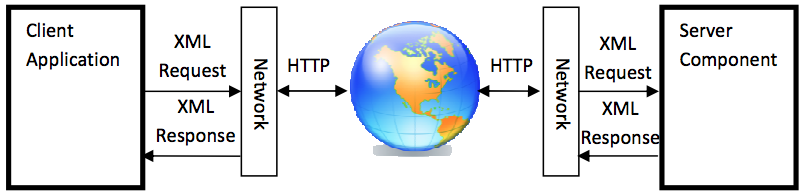
\includegraphics[width=0.7\linewidth]{Abbildungen/clientServerKommunikation.png}
	\captionof{figure}[clientServerKommunikation.png]{Generische Client-Server Kommunikation bei Webservices}
	\label{fig:clientServerKommunikation.png}
\end{minipage}
\vspace{1em}

Abbildung \ref{fig:clientServerKommunikation.png} entspricht im wesentlichen der klassischen Client-Server Kommunikation im Web. Exemplarisch werden XML-Daten übertragen, was die zugrunde liegende Idee der Webservices illustriert: die Übertragung anderer Daten als Webseiten mittels HTTP.

\citet{wilde11} reden von zwei etablierten \glqq Geschmäckern\grqq{} (flavors) in der Webservice-Welt: SOAP und REST. Die erste Geschmacksrichtung bedeutet Webservices \glqq auf Basis von SOAP, WSDL und den WS-*Standards - bzw. [...] deren Architektur\grqq{} \citep{tilkov11}. Hier wird also ein XML-basierter Technologiestack beschrieben. REST hingegen ist ein Architekturstil, der 2000 in der Dissertation von \citeauthor{fielding00} vorgestellt wurde. Der Versuch, beide Varianten direkt gegenüber stellen zu wollen, ist ein \glqq [...] klassischer Apfel-Birnenvergleich: ein konkretes XML-Format gegen einen abstrakten Architekturstil\grqq{} \citep{tilkov11}.

Vor einer detaillierteren Diskussion von SOAP und REST wird zur Einordnung eine grundlegende Unterscheidung der Ansätze vorgestellt. Gemeinsam ist beiden, dass HTTP als Transportprotkoll zur Übertragung der Frage (Request) verwendet wird, die vom Server (Response) beantwortert werden soll. HTTP wiederum besteht aus einem Header und einem Entity-Body zur Übertragung von Daten. \citet{richardson07} haben zwei Leitfragen herausgearbeitet, die von den jeweiligen Ansätzen unterschiedlich beantwortet werden: wo in diesem Paket sagt der Client dem Service, mit welchen Daten (Fokusinformation) was (Methodeninformation) gemacht werden soll?

Die Fokusinformation sagt aus, für welche Datenelemente sich der Client interessiert (z.B. ein Artikel eines Onlineshops). Bei REST ist dies der URI zu entnehmen (z.B. http://onlineshop.com/artikel/pc). Bei SOAP steht diese Information in einer XML-Datei welche Entity-Body übertragen wird; die sogenannte Payload. Die Methodeninformation sagt aus, was mit dem identifizierten Datenelement geschehen soll (Bsp: lege einen neuen PC-Artikel an). Bei REST steht dies im Methodenfeld der HTTP-Headers, bei SOAP wieder im Entity-Body. Daraus lässt sich als grundlegender Unterschied ableiten: SOAP verwendet HTTP nur als Transportprotokoll, REST auch dessen Ausdruckskraft \citep{wilde11}.

\subsubsection{SOAP}
Bei SOAP-Web Services wird ein \ac{RPC} durchgeführt. Dabei handelt es sich um eine generelle Technik zur Realisierung von Systemverteilung. Ein System ruft die Funktion eines Systems aus einem anderen Adressraum auf. SOAP ist ein XML-basiertes Umschlagsformat, welches wiederum die Beschreibung eines Methodenaufrufs in XML-Form enthält. Bei SOAP-Web Services werden also \ac{RPC}s über HTTP getunnelt \citep{wilde11}. Das ist Konvention, aber keine Notwendigkeit: der SOAP-Umschlag ist transportunabhängig, könnte also auch von anderen Protokollen als HTTP übertragen werden \citep{tilkov11}. Solange es sich bei dem Transportprotokoll um eine Webtechnologie handelt, wird die Webservicedefinition nicht verletzt.

Wie die Beschreibung des \ac{RPC} aussehen muss, definiert die \ac{WSDL}. Jeder SOAP basierte Service stellt eine maschinenverarbeitbare \ac{WSDL}-Datei bereit. Darin werden die aufrufbaren Methoden, deren Argumente und Rückgabetypen beschrieben. Außerdem werden Schemata der XML-Dokumente festgehalten, die der Service akzeptiert und versendet \citep{richardson07}.

Es existieren eine Vielzahl von Middleware-Interoperabilitätsstandards, die mit dem \glqq WS-\grqq{} Prefix versehen sind. Diese sind \glqq XML-Aufkleber\grqq{} für den SOAP-Umschlag, die HTTP-Headern entsprechen \citep{richardson07}. Sie erweitern die Ausdrucksmöglichkeit des SOAP-Formats \citep{wilde11}. Beispielsweise erlaubt WS-Security die Berücksichtigung von Sicherheitsaspekten bei der Client-Server Kommunikation. Eine Übersicht der existierenden Standards ist dem Wiki für Webservices \citet{webServiceWiki09} zu entnehmen.

\subsubsection{REST}
\begin{quote}
\glqq Eine Architektur zu definieren bedeutet zu entscheiden, welche Eigenschaften das System haben soll, und eine Reihe von Einschränkungen vorzugeben, mit denen diese Eigenschaften erreicht werden können.\grqq{} \citep{tilkov11}
\end{quote}

Dies ist in der Dissertation von \citeauthor{fielding00} geschehen, in der REST als Architekturstil definiert wird. Ein Architekturstil ist ein stärkerer Abstraktionsgrad als eine Architektur. Beispielsweise ist das Web eine HTTP-Implementierung von REST \citep{tilkov11}. Tatsächlich wurden die Einschränkungen von REST aber dem Web entnommen, indem \citeauthor{fielding00} es post-hoc als lose gekoppeltes, dezentralisiertes Hypermediasystem konzeptualisiert \citep{wilde11} und dann von diesem Konzept abstrahiert hat. Einen Webservice nach dem REST-Architekturstil zu implementieren passt ihn dem Wesen des Webs an und nutzt dessen stärken \citep{tilkov11}.

Entsprechend \citeauthor{tilkov11}s Architekturdefinition werden im Folgenden die Einschränkungen von REST sowie die daraus resultierenden Eigenschaften besprochen.

\textbf{Einschränkungen}\\
Einschränkungen sind - in eigenen Worten - Implementierungskriterien. Während \citeauthor{fielding00} in seiner theoretischen Abhandlung explizit vier solcher Kriterien nennt, basiert die folgende Auflistung auf der praxiserprobten Variante der Sekundärliteratur \citep{wilde11, tilkov11}.

\begin{compactitem}
\item \textbf{Ressourcen mit eindeutiger Identifikation}: \glqq Eine Ressource ist alles, was wichtig genug ist, um als eigenständiges Etwas referenziert zu werden\grqq{} \citep{richardson07}. Identifiziert werden sie im Web durch URIs, die einen globalen Namensraum darstellen.  Es ist hervorzuheben, dass Ressourcen nicht das gleiche sind wie die Datenelemente aus der Persistenzschicht einer Anwendung. Sie befinden sich auf einem anderen Abstraktionsniveau. Beispiel: eine Warenkorbressource kann eine Auflistung von Artikeln sein, welche allerdings nicht einzeln als Ressource ansprechbar sind. \citeauthor{tilkov11} nimmt in diesem Zusammenhang eine Typisierung von Ressourcen vor. Von den sieben verschiedenen Ressourcentypen sind folgende im Rahmen der Fragestellung interessant:
\begin{enumerate}[a.]
\item Bei einer \textbf{Projektion} wird die Informationsmenge verringert, indem eine sinnvolle Untermenge der Attribute einer abgerufenen Ressource gebildet wird. Zweck ist die Reduktion der Datenmenge. Beispiel: Weglassen der Beschreibungstexte von Warenkorbpositionen (d.h. ein Artikel im Warenkorb).
\item Die \textbf{Aggregation} ist das Gegenteil. Hier werden Attribute unterschiedlicher Ressourcen zur Reduktion der Anzahl notwendiger Client/Server Interaktionen zusammengefasst. Beispiel: Hinzufügen der Versandkosten beim Abruf der Warenkorbpositionen.
\item \textbf{Aktivitäten} sind Ressourcen, die sich aus Prozessen ergeben, wie etwa ein Schritt innerhalb einer Verarbeitung. Beispiel: Ein Schritt einer nicht abgeschlossenen Konfiguration.
\end{enumerate}
\item \textbf{Hypermedia} beschreibt das Prinzip verknüpfter Ressourcen. So wird dem Client ermöglicht, neue Ressourcen zu entdecken oder bestimmte Prozesse anzustoßen. Beispiel: Zur einer Bestellbestätigungsressource wird der zugehörige Stornierungslink hinzugefügt.
\item \textbf{Standardmethoden/uniforme Schnittstelle}: Oben wurde beschreiben, dass jede Ressource durch (mindestens) eine ID identifiziert wird. Jede URI unterstützt dabei den gleichen Methodensatz, welche mit den HTTP-Methoden korrespondieren. Das bedeutet - übertragen auf die objektorientierte Programmierung: jedes Objekt implementiert das gleiche Interface. Folgende Teilmenge der neun verfügbaren HTTP-Methoden finden in der Literatur am häufigsten Erwähnung:
\begin{enumerate}[a.]
\item \textbf{GET:} Das Abholen einer Ressource.
\item \textbf{PUT:} Das Anlegen oder Aktualisieren einer Ressource. Je nachdem, ob unter dieser URI bereits eine Ressource existiert.
\item \textbf{POST:} Bedeutet im engeren Sinne das Anlegen einer Ressource unter einer URI, die vom Service bestimmt wird. Im weiteren Sinne kann durch Post ein Prozess angestoßen werden.
\item \textbf{Delete:} Das Löschen einer Ressource.
\end{enumerate}

\vspace{1em}
\begin{minipage}{\linewidth}
	\centering
	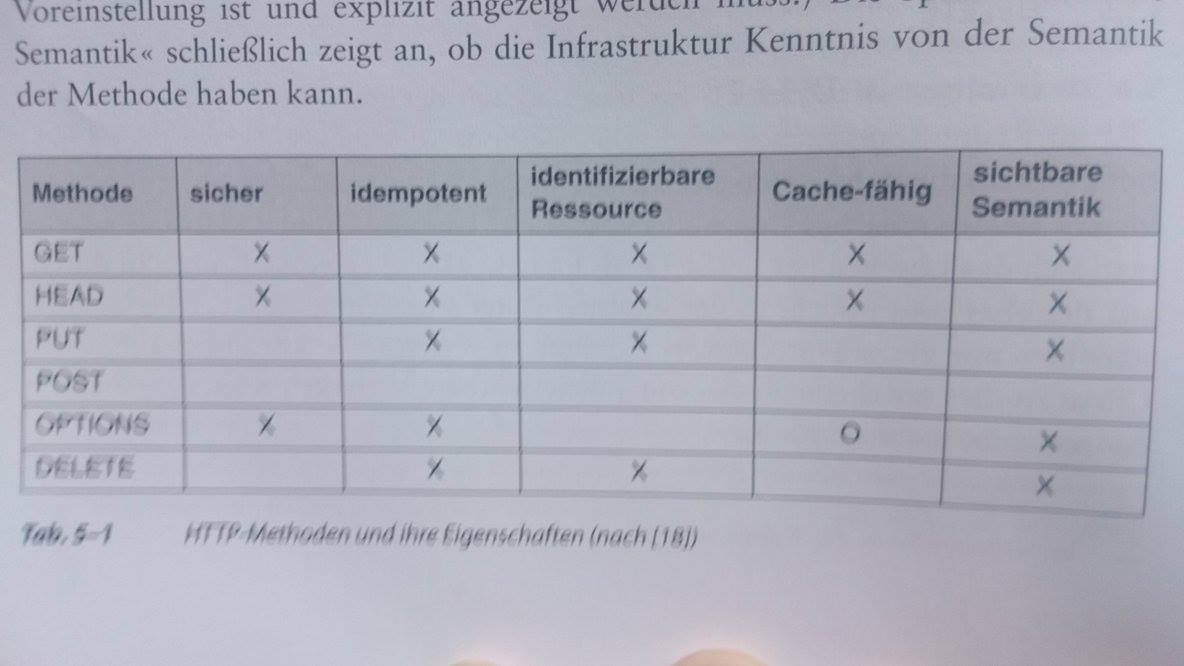
\includegraphics[width=0.7\linewidth]{Abbildungen/restMethoden.jpg}
	\captionof{figure}[restMethoden]{HTTP-Methoden und ihre Eigenschaften
	\footnote{Relevante Attribute im Rahmen der Fragestellung: \glqq sicher\grqq{} bedeutet nebenwirkungsfrei, d.h. kein Ressourcenzustand ändert sich durch diese Methode. \glqq Idempotent\grqq{} bedeutet, dass das Resultat der Methode bei Mehrfachausführung das gleiche ist. \glqq Identifizierbare Ressource\grqq{} bedeutet, dass die URI garantiert eine Ressource identifiziert.}
	(Quelle: \citet{tilkov11})}
	\label{fig:restMethoden}
\end{minipage}
\vspace{1em}

Abbildung \ref{fig:restMethoden} fast die Eigenschaften der Methoden aus der HTTP-Spezifikation 1.1 zusammen. Die Implementierung einer Methode muss dem erwarteten Verhalten aus dieser Spezifikation entsprechen. Die Praxis zeigt, dass nur die Methoden unterstützt werden, die für die jeweilige Ressource sinnvoll sind. Abbildung \ref{fig:restMethoden} macht außerdem klar, dass es für POST keinerlei Garantien gibt. Da nicht eindeutig ist, ob über POST eine Ressource erstellt oder ein Prozess angestoßen wird, sehen \citeauthor{richardson07} hierin eine Verletzung der uniformen Schnittstelle. Dies bedeutet in der Praxis: was bei einem Post passiert, ist nicht der HTTP-Spezifikation, sondern der API-Beschreibung des Webservice zu entnehmen.
\item \textbf{Ressourcen und Repräsentationen:} Beschreibt die Darstellungen einer Ressource in einem definierten Format. Der Client bekommt nie die Ressource selbst, sondern nur eine Repräsentation derer zu sehen. In der Praxis wird meist eine  serialisierte Variante eines Objektes als JSON zur Verfügung gestellt. Beispiel: Bereitstellung einer Bestellbestätigung als PDF und HTML.
\item \textbf{Statuslose Kommunikation} bedeutet die Nichtexistenz eines serverseitig abgelegten, transienten, clientspezifischen Status über die Dauer eines Requests hinweg. Der Service benötigt also nie Kontextinformationen zur Bearbeitung eines Requests. Beispiel: Ein Warenkorb wird nicht in einem Sessionobjekt, sondern als persistentes Datenelement gehalten.
\end{compactitem}

Diese Auflistung legt folgende Frage nahe: ist ein Webservice nur dann REST-konform, wenn alle Kriterien erfüllt werden? Was ist mit einem Webservice, der allen Einschränkungen gerecht wird, jedoch Ressourcen nur als JSON ausliefert - ein in der Praxis häufig anzutreffender Fall; und dennoch ein Verstoß gegen die Forderung nach unterschiedlichen Repräsentationen. Aus diesem Grund existiert das \glqq Richardson Maturity Model\grqq{}, welches die abgestufte Bewertung eines Webservices nach dessen REST-Konformität erlaubt. Es wird im Auswertungsteil vorgestellt und zur Evaluierung der Implementierung genutzt.

\textbf{Eigenschaften}\\
Aus den vorgestellten Kriterien resultieren folgende Eigenschaften \citep{tilkov11},  welche die Vorteile REST-basierter Webservices gegenüber der SOAP-Konkurrenz darstellen \citep{richardson07}:

\begin{compactitem}
\item \textbf{Lose Kopplung:} Beschreibt isolierte Systeme mit größtmöglicher Unabhängigkeit, die über Schnittstellen miteinander kommunizieren. Hierzu tragen die Standardmethoden bei.
\item \textbf{Interoperabilität:} Beschreibt die Möglichkeit der Kommunikation von Systemen unabhängig von deren technischen Implementierung. Dies ergibt sich durch die Festlegung auf Standards. Bei der Anwendung von REST auf Webservices sind dies die Webstandards (z.B. HTTP, URIs).
\item \textbf{Wiederverwendbarkeit}: Jeder Client, der die Schnittstelle eines REST-basierten Service verwenden kann, kann auch jeden anderen beliebigen REST-basierten Service nutzen - vorausgesetzt, das Datenformat wird von beiden Seiten verstanden.
\item \textbf{Performance und Skalierbarkeit}: Webservices sollen schnell antworten, unabhängig von der Anzahl von Anfragen in einem definierten Zeitraum. Dies wird durch Cachebarkeit (siehe HTTP-Methodenspezifikation) und Zustandslosigkeit erreicht. Da der Service keinen clientspezifischen Kontext aufbauen muss, müssen aufeinanderfolgende Requests nicht vom gleichen System beantwortet werden.
\end{compactitem}
\pagebreak

\textbf{Kurzfazit}\\
In der generellen Ausrichtung ist REST Ressourcenorientiert während SOAP aufgrund von \ac{RPC}s Methodenorientiert ist. Um REST zu implementieren, müssen Kriterien erfüllt werden. Die einzige technische Voraussetzung ist das Bereitstellen von Funktionen, die auf verschiedene URIs reagieren und HTTP verarbeiten können. Bei SOAP ist HTTP nur das Transportprotokoll. Die Verarbeitung des Inhalts erfordert einen weiteren Technologiestack.

\subsection{eCommerce}

Im Folgenden wird durch die Charakterisierung des Begriffs eCommerce ein Andwendungsrahmen für eShops hergestellt. Deren softwaretechnische Umsetzung wird durch eShop-Systeme realisiert. Durch eine Kategorisierung der Systeme nach Anbieterstrategie wird abschließend die Menge der Open-Source-Lösungen für eine Konfiguratorintegration identifiziert.

\subsubsection{Anwendungsrahmen}
eShops gehören zur Domäne des elektronischen Handels (eCommerce). eCommerce ist \glqq die elektronisch unterstützte Abwicklung von Handelsgeschäften auf der Basis des Internet\grqq{} \citep{schwarze02}. Je nachdem, welche Marktpartner an dem Handelsgeschäft teilnehmen, werden verschiedene Formen des eCommerce unterschieden. Die in Abbildung \ref{fig:eCommerceGrundformen} fett hervorgehobenen Varianten werden von \citet{meier12} als \glqq die zwei Geschäftsoptionen des eCommerce\grqq{} bezeichnet: \ac{B2C} und \ac{B2B}. Bei \ac{B2C} erfolgt der Handel von Produkten und Dienstleistungen zwischen Unternehmen and Endverbraucher, bei \ac{B2B} zwischen Unternehmen.

\vspace{1em}
\begin{minipage}{\linewidth}
	\centering
	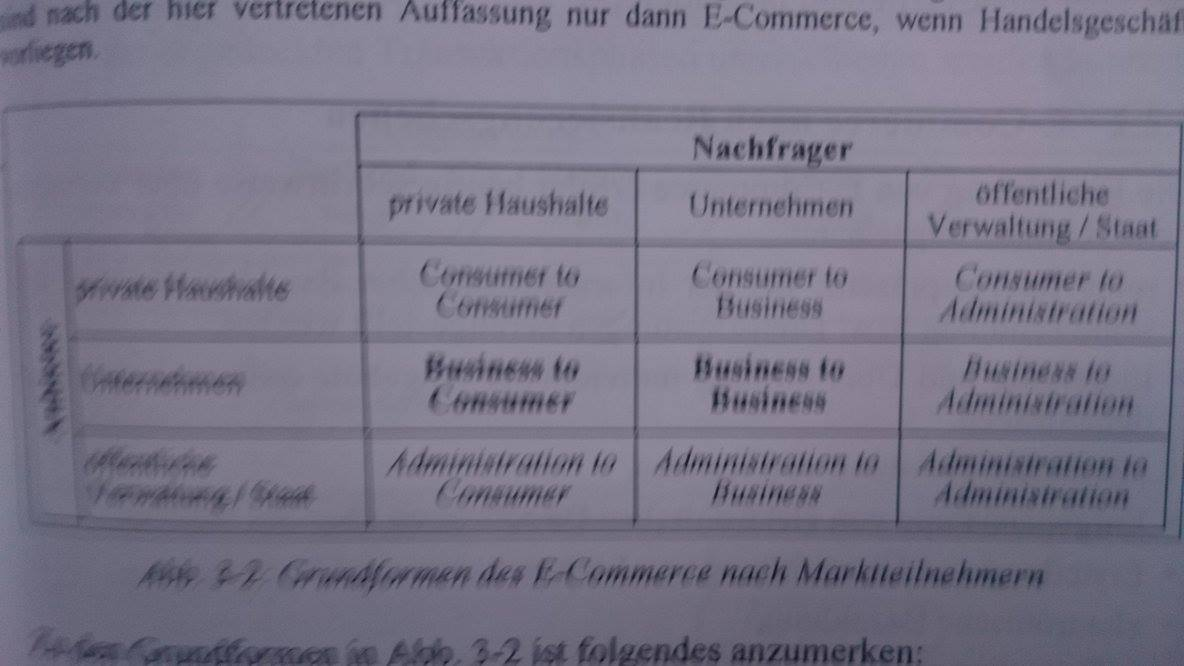
\includegraphics[width=0.7\linewidth]{Abbildungen/eCommerceGrundformen.jpg}
	\captionof{figure}[eCommerceGrundformen]{Grundformen des eCommerce nach Marktpartnern (Quelle: \citet{schwarze02})}
	\label{fig:eCommerceGrundformen}
\end{minipage}
\vspace{1em}

Für die Umsetzung von eCommerce existieren unterschiedliche Geschäftsmodelle. \citet{timmers98} nennt 11 verschiedene Formen. eShops sind eine eine davon. Es handelt sich dabei um ein \glqq Geschäftsmodell der Angebotsveröffentlichung, bei dem ein Anbieter seine Waren oder Dienstleistungen über das Web den Nachfragern offeriert\grqq{} \citep{bartelt00}.

Ein eShop bildet den traditionellen Einkaufsvorgang nach: Kunden können mittels einer Katalog- oder Suchfunktion über den Produktbestand navigieren. Produkte können ausgewählt und ausführliche, mit Medien angereicherte Beschreibungen abgerufen werden. Wunschartikel werden einem virtuellen Warenkorb hinzugefügt. Ist die Produktauswahl abgeschlossen, begibt sich der Kunde zur \glqq Kasse\grqq{}, wo die Zahlungsmodalitäten erledigt werden \citep{boles00}. Ein eShop beschreibt das Geschäftsmodell, jedoch noch nicht dessen Umsetzung als Softwaresystem. Diese wird als eShop-System bezeichnet \citep{boles00} und im Folgenden behandelt.

\subsubsection{eShop-Systeme}
\glqq eShop-Systeme sind Software-Systeme, die den Aufbau, die Verwaltung und den Einsatz von eShops unterstützen\grqq{} \citep{boles00}. Abbildung \ref{fig:eShopGrobarchitektur} zeigt die Grobarchitektur eines eShop-Systems nach \citeauthor{meier12}. Darin wird die Unterteilung zwischen Storefront und Backfront deutlich, welche in der Terminologie realer Shopsysteme als Front- und Backend bezeichnet werden \citep[vgl.][]{shopwareDoku}. Das Frontend ist der Interaktionsraum der Kunden, das Backend der administrative Bereich des Shopbetreibers.

\vspace{1em}
\begin{minipage}{\linewidth}
	\centering
	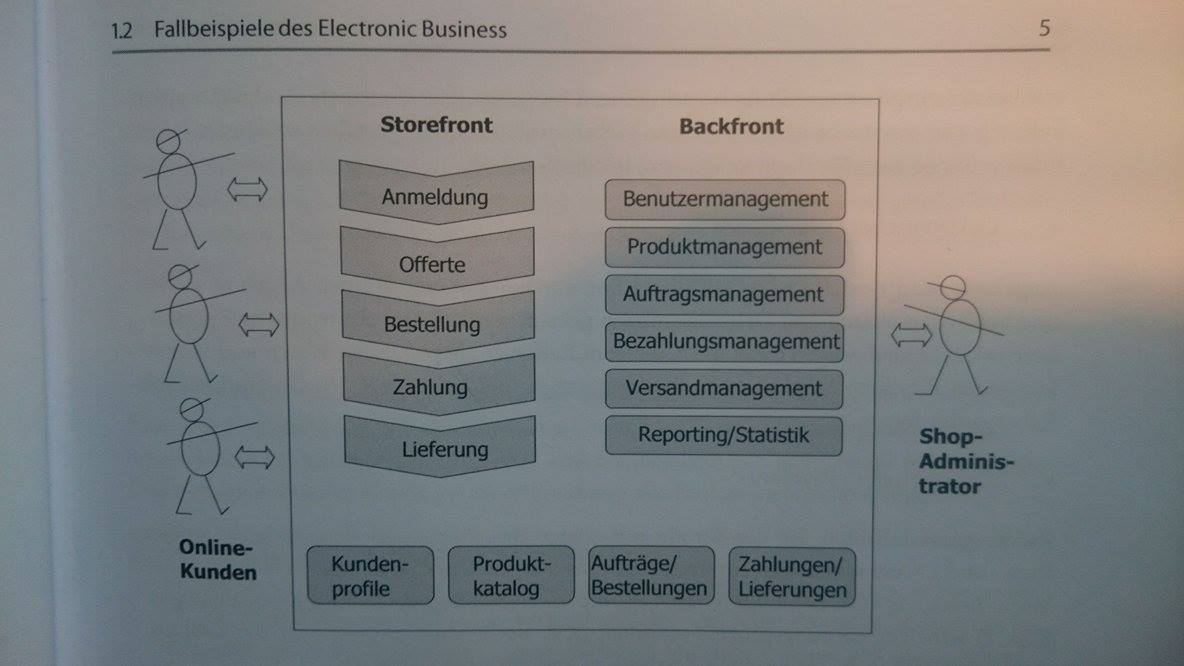
\includegraphics[width=0.7\linewidth]{Abbildungen/eShopGrobarchitektur.jpg}
	\captionof{figure}[eShopGrobarchitektur]{Grobarchitektur eines eShop-Systems (Quelle: \citet{meier12})}
	\label{fig:eShopGrobarchitektur}
\end{minipage}
\vspace{1em}

Die Hauptaufgaben eines eShop-Systems sehen \citet{boles00} in den Bereichen Merchandising (z.B. Management von hierarchisch strukturierten Produktkatalogen, Beeinflussung des Shopdesigns), Auftragsbearbeitung (z.B. Festlegung der Abarbeitungs-Pipeline, Integration von Bezahlverfahren) und Sonstiges (z.B. die Kopplung mit externen ERP-Systemen). Der konkrete Funktionsumfang hängt vom  gewählten eShop-System ab.

Die Systeme sind nach Strategie der Anbieter kategorisierbar:
\begin{compactitem}
\item \textbf{Open-Source}-Systeme sind kostenlos verfügbar. Sie bieten völlige Gestaltungsfreiheit, aber keinen Herstellersupport. Die Dokumentationen sind schwächer und der Funktionsumfang geringer als bei kostenpflichtigen Alternativen. Andererseits existieren Communities, die Unterstützung bieten und die Entwicklung von Erweiterungen vorantreiben \citep{stahl15}. Beim kommerziellen Handel der modularen Erweiterungen auf shopspezifischen Stores liegt auch eine der wesentlichen Erlösquellen der Open-Source Strategie (z.B. der Addon Marketplace der \citeauthor{prestashopAddons} oder das Extensionverzeichnis der \citeauthor{opencartExtensions}).
\item \textbf{Kauf-Lösungen} können kostenpflichtig lizensiert werden (z.B. \citeauthor{shopwarePricing}). Sie bieten Herstellersupport, zusätzliche Dienstleistungen (z.B. Installation des Shops) und einen höheren Funktionsumfang (z. B. Schnittstellen zu verschiedenen Warenwirtschaftssystemen oder Zahlungsdienstleistern) \citep{stahl15}. Die Hersteller bieten verschiedene Editionen mit teilweise erheblichen Preisunterschieden an (Bsp.: die Preisdifferenz der Magento Enterprise Edition zu Enterprise Premium liegt bei über 35.000 \$, \citealp[vgl][]{fwpShop}).
\begin{enumerate}[a.]
\item Im Rahmen eines Dual-License-Modells ist eine Open-Source \textbf{Community Edition} Teil des Editionsspektrums \citep{t3n14} (vgl. das Shopangebot der \citeauthor{magentoShops}, \citeauthor{shopwarePricing} oder \citeauthor{oxidShops}). Durch den offenen Quellcode existiert auch hier der Handel modularer Erweiterungen, von dem auch die kostenpflichtigen Varianten profitieren (vgl. der Plugin Store der \citeauthor{shopwarePluginStore}). Die Codebasis aller Editionen ist gleich. Daher kann später zu einer Kauf-Lösung migriert werden. Das bietet Flexibilität für wachsende Shopanforderungen.
\end{enumerate}
\item \textbf{Miet-Shops} entsprechen einer Cloud-Lösung als Software-as-a-Service (z.B. \citeauthor{stratoWebshops}, \citeauthor{shopify15}). Die technische Infrastruktur wird vom Provider zur Verfügung gestellt. Systemwartung, Bereitstellung der Shopsoftware und Hosting werden unter dem Mietpreis abgerechnet. \citet{stahl15} bewertet diese Variante als Einstiegslösung mit geringer Gestaltungsfreiheit.
\item \textbf{Eigenentwicklungen} eignen sich für individuelle Bedürfnisse, wenn die Standardsysteme die Anforderungen nicht mehr erfüllen \citep{stahl15, graf14}.
\end{compactitem}

Aus dieser Darstellung sind die (zumindest initial) kostenfreien Varianten ersichtlich: reine Open-Source eShop-Systeme sowie die Community-Editionen der Dual-License Modelle. Eine Anbieterübersicht ist \citet{t3n14} zu entnehmen. Eine Kategorisierung der Systeme nach Anforderungsklassen ist \citet{graf14} zu entnehmen.

\pagebreak
\section{Analyse}
\label{section:Analyse}

Die Tacton Systems AB (Tacton) wurde 1998 als Spin-Off des Schwedischen Instituts für Informatik (SICS) gegründet \citep{tactonProductOverview}. In der Forschungseinrichtung wurde als Resultat der Untersuchungen im Bereich Wissensbasierte Systeme und Künstliche Intelligenz der Tacton Produktkonfigurator entwickelt. Dieser interaktive Konfigurator ist die Basis der verschiedenen Produkte der Firma. Tacton bietet Lösungen im Bereich Vertriebskonfiguration und Design Automation (Automatisierung der Konstruktion in CAD-Systemen) \citep{tactonAbout}.

\subsection{Konfigurationsmodell}
\label{subsection:Konfigurationsmodell}
Das in Abschnitt \ref{subsubsection:wissenrepraesentation} vorgestellte Visualisierungskonzept abstrahiert Konfigurationswissen in einen Struktur- und einen Regelteil. Im Tacton-Konfigurationsmodell wird ebenfalls abstrahiert, jedoch in andere Domänen \citep{tactonModeling}:

\begin{enumerate}[(a)]
\item \label{strukturinformation} Strukturinformation: wie ist das Produkt hierarchisch aufgebaut?
\item \label{komponenteninformation} Komponenteninformation: aus was ist es aufgebaut?
\item \label{constraintinformationen} Constraintinformationen: wann ist das Produkt korrekt?
\item \label{ausfuehrungsinformationen} Ausführungsinformationen: welche Fragen bekommt der Nutzer in welcher Reihenfolge gestellt?
\end{enumerate}

Dabei sind zwei Sachverhalte feststellbar:
\begin{enumerate}[(1)]
\item \label{enum:componentsConfiguration} Typisch für einen modellbasierten Konfigurator wird Produktwissen und Problemlösungswissen bei der Wissensmodellierung separiert. Beispiel: ein Constraint, der die Kompatibilität bestimmter Betriebssysteme mit einer bestimmten Anzahl Prozessorkerne ausdrückt, soll wirken, auch ohne die konkreten CPU-Typen (z.B. Intel i7) zu kennen. Darum ist die Rede von generischen Constraints: sie beziehen sich auf alle Komponenten eines Typs \citep{felferning14}.
\item \label{enum:execution} Im Konfigurationsmodell wird auch die Nutzerinteraktion festgelegt. Damit geht der Funktionsumfang eines Tacton-Modells über die Definition aus Abschnitt \ref{subsubsection:begriffsuberblick} hinaus.
\end{enumerate}

Bei der UML-Wissensrepräsentation aus Abschnitt \ref{subsubsection:wissenrepraesentation} wurden die Domänen \eqref{komponenteninformation} und \eqref{strukturinformation} als Diagramm ausgedrückt sowie \eqref{constraintinformationen} als Tabelle. Tacton wählt eine andere Aufteilung. \eqref{komponenteninformation} wird unter dem Begriff \glqq Components\grqq{} umgesetzt, \eqref{strukturinformation} und \eqref{constraintinformationen} unter dem Begriff \glqq Configuration\grqq{}. Components und Configuration setzen gemeinsam den Sachverhalt \eqref{enum:componentsConfiguration} um und werden im Folgenden besprochen. Daraufhin wird die \glqq Execution\grqq{} besprochen, welche Sachverhalt \eqref{enum:execution} umsetzt.


\subsubsection{Components und Configuration}

\vspace{1em}
\begin{minipage}{\linewidth}
	\centering
	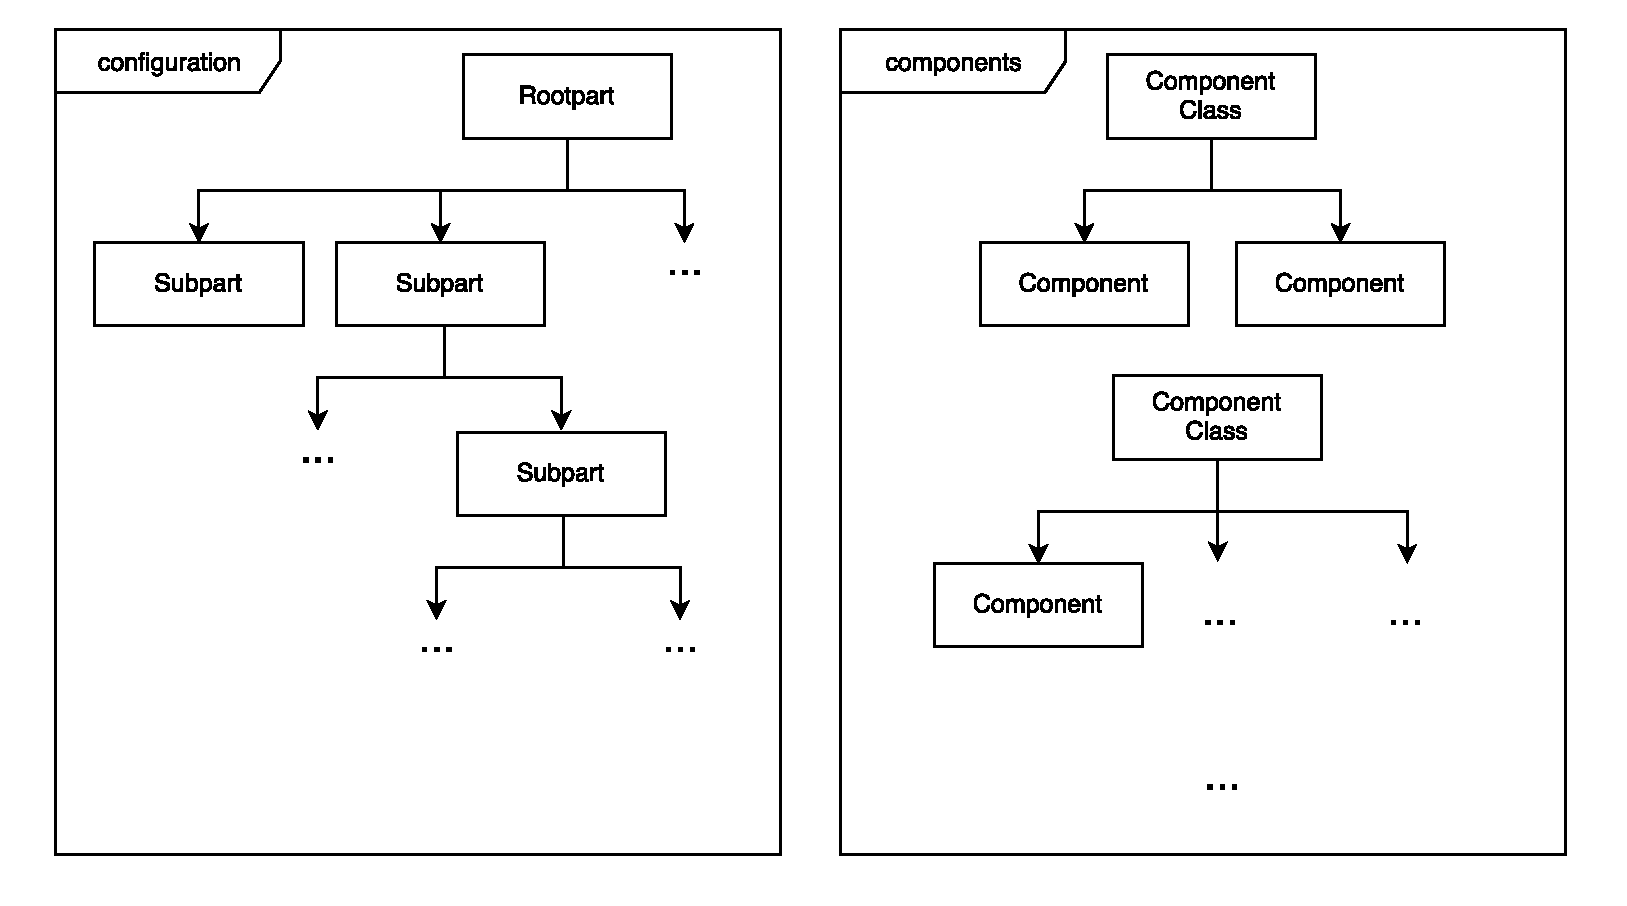
\includegraphics[width=1\linewidth]{Abbildungen/tactonModellHighLevel.pdf}
	\captionof{figure}[tactonModellHighLevel]{High-Level Architektur des Tacton-Konfigurationsmodells}
	\label{fig:tactonModellHighLevel}
\end{minipage}
\vspace{1em}

Abbildung \ref{fig:tactonModellHighLevel} zeigt das High-Level-Konzept der Modellarchitektur. Unter 'configuration' wird die Produktstruktur als hierarchischer Baum  von 'Part'-Objekten dargestellt. Jeder Part kann Constraints enthalten, die sich auf den Knoten selbst und alle seine Kinder beziehen. Ein Part ist ansonsten nur ein Komponentenplatzhalter. Noch ist keine Information darüber hinterlegt, welches Bauteil dort eigentlich verkörpert wird. Abbildung \ref{fig:tactonModellHighLevelNotebook} veranschaulicht das Konzept am Notebook-Beispiel.

\vspace{1em}
\begin{minipage}{\linewidth}
	\centering
	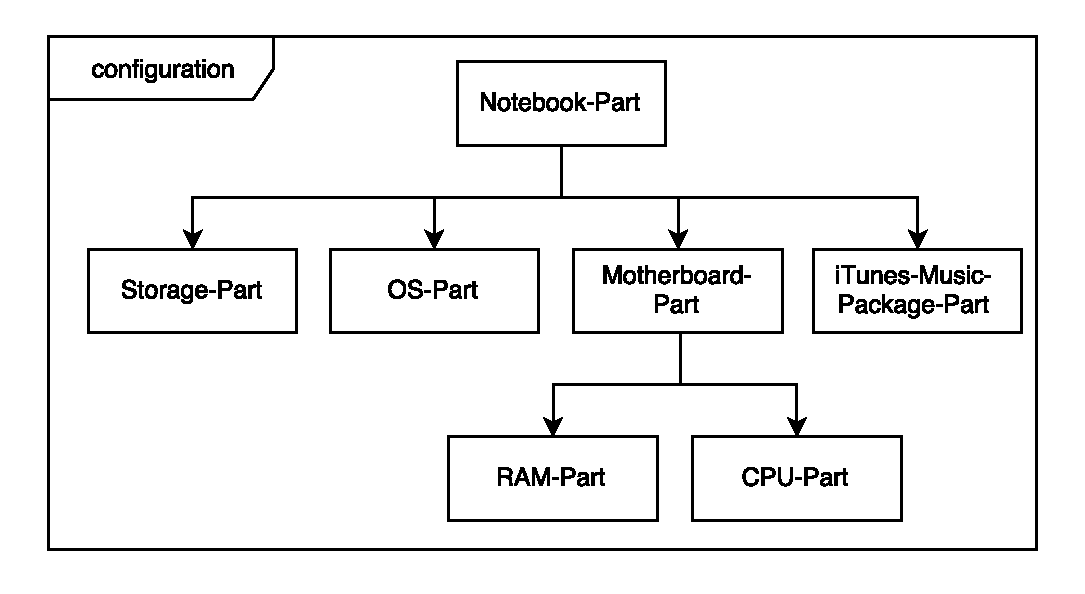
\includegraphics[width=0.7\linewidth]{Abbildungen/tactonModellHighLevelNotebook.pdf}
	\captionof{figure}[tactonModellHighLevelNotebook]{Part-Struktur der Notebook-Konfiguration}
	\label{fig:tactonModellHighLevelNotebook}
\end{minipage}
\vspace{1em}

Die Informationen über die eben erwähnten Bauteile (d.h. Komponententypen) werden isoliert unter 'components' definiert (Abbildung \ref{fig:tactonModellHighLevel}). Ein Bauteil wird in 'Component Classes' und 'Components' abstrahiert. Das ist analog zu  Komponententypen, die in einer Generalisierungsbeziehung zueinander stehen (siehe Kapitel \ref{subsubsection:wissenrepraesentation}). Hier wurde eine Terminologie gewählt, die Supertyp und Subtyp unterscheidbar macht. Eine Component Class (z.B. ein 'RAM') wird durch Eigenschaften beschrieben, die als Features bezeichnet werden. Jedes Feature besitzt einen Namen (z.B. 'memory') und einen Wertebereich (z.B. [2GB, 4GB]), welche als Domain bezeichnet wird. Wertebereiche können Integer, Float, Boolean, andere Component Classes oder selbstdefinierte Enumerationen sein. Components (z.B. eine 'SSD') sind das, was eine Component Class (z.B. ein 'Storage') konkret sein kann. Sie übernehmen alle Features der übergeordneten Component Class und besitzen konkrete Werte ('Values') aus dem jeweiligen Wertebereich.

\vspace{1em}
\begin{minipage}{\linewidth}
	\centering
	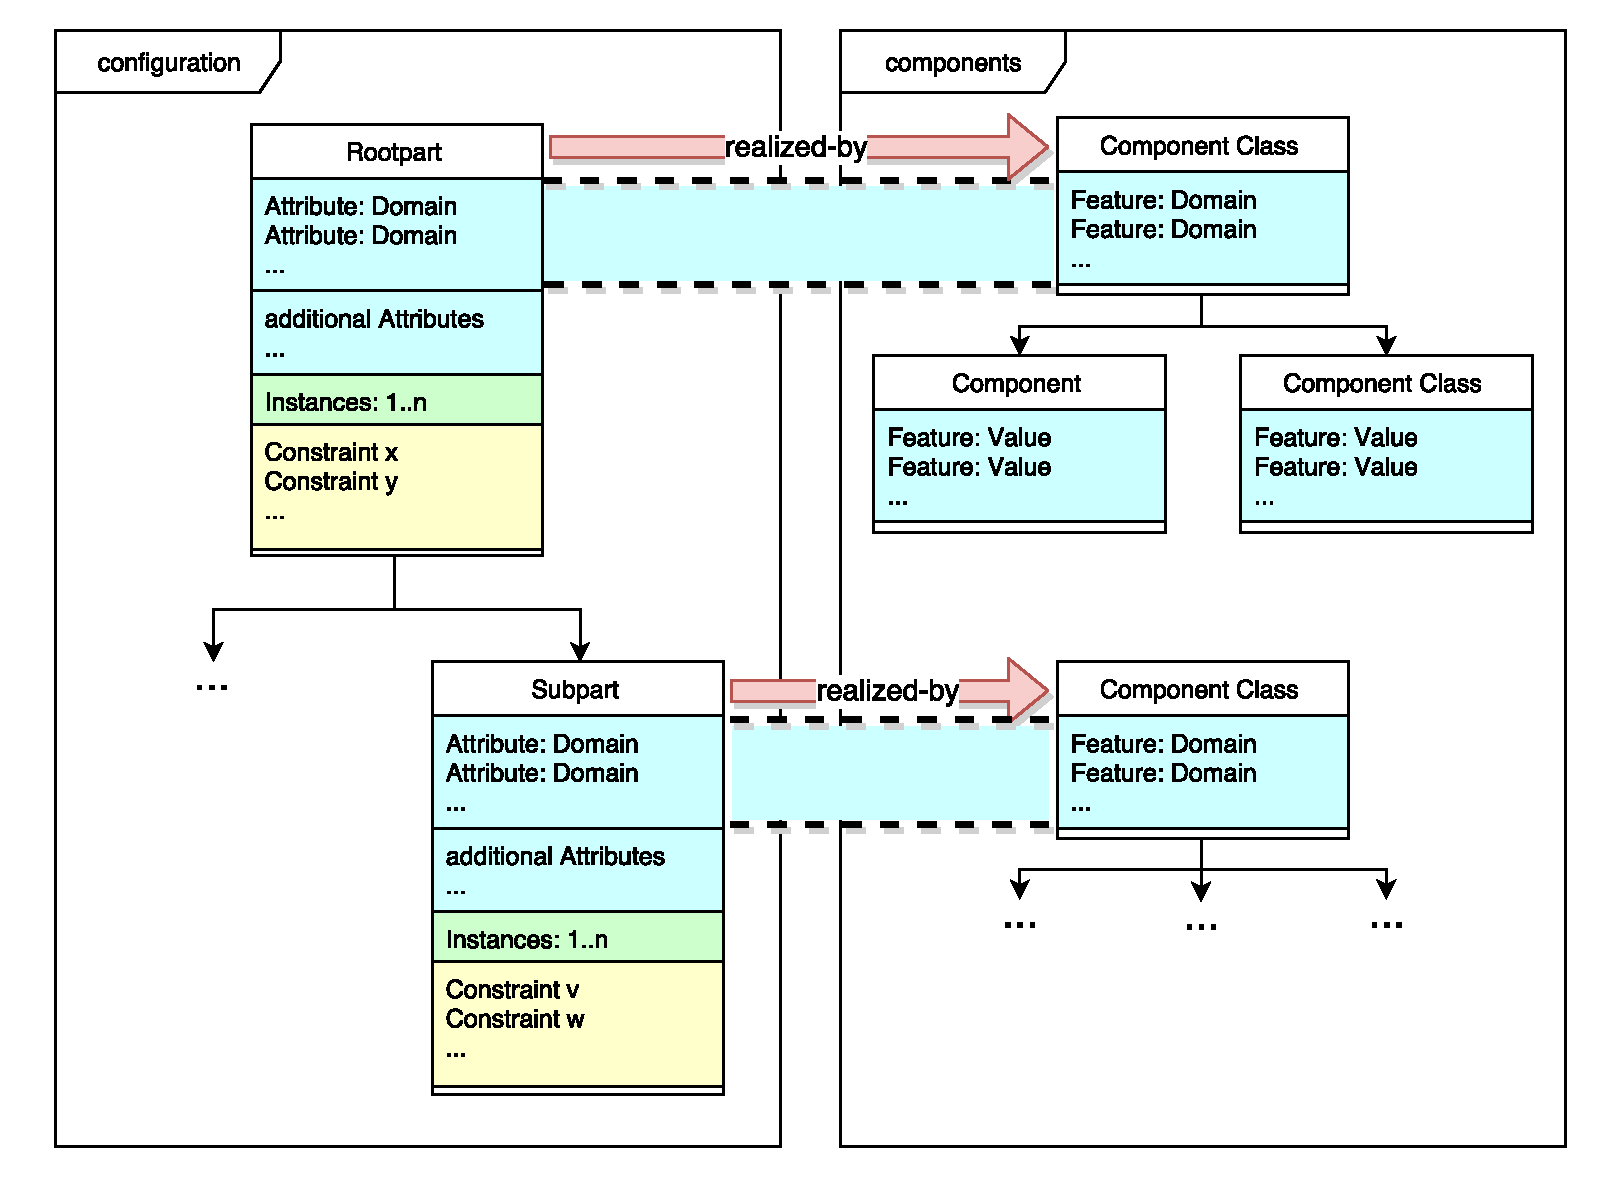
\includegraphics[width=1\linewidth]{Abbildungen/tactonModellLowLevel.pdf}
	\captionof{figure}[tactonModellLowLevel]{Zuordnung von Parts und Component Classes.}
	\label{fig:tactonModellLowLevel}
\end{minipage}
\vspace{1em}

Abbildung \ref{fig:tactonModellLowLevel} zeigt die Zuordnung zwischen Parts und Component Classes via Verzeigerung. Einem Part wird eine Component Class durch eine 'realized-by' Beziehung zugeordnet. Dem Part werden dabei die Features der entsprechenden Component Class vererbt (türkis dargestellt). Nur werden sie zur besseren Differenzierung beim Part nicht mehr als Features, sondern als Attribute bezeichnet. Für einen Part können auch noch zusätzliche Attribute definiert werden ('additional Attributes'), falls notwendig. Die Angabe 'Instances' (grün dargestellt) entspricht den Kardinalitäten in Abschnitt \ref{fig:tactonModellLowLevel}. Constraints (gelb dargestellt) werden als logische Ausdrücke formuliert. Sie bestehen aus Attributwerten, die mit mathematischen Zeichen in Relation gebracht werden.

\vspace{1em}
\begin{minipage}{\linewidth}
	\centering
	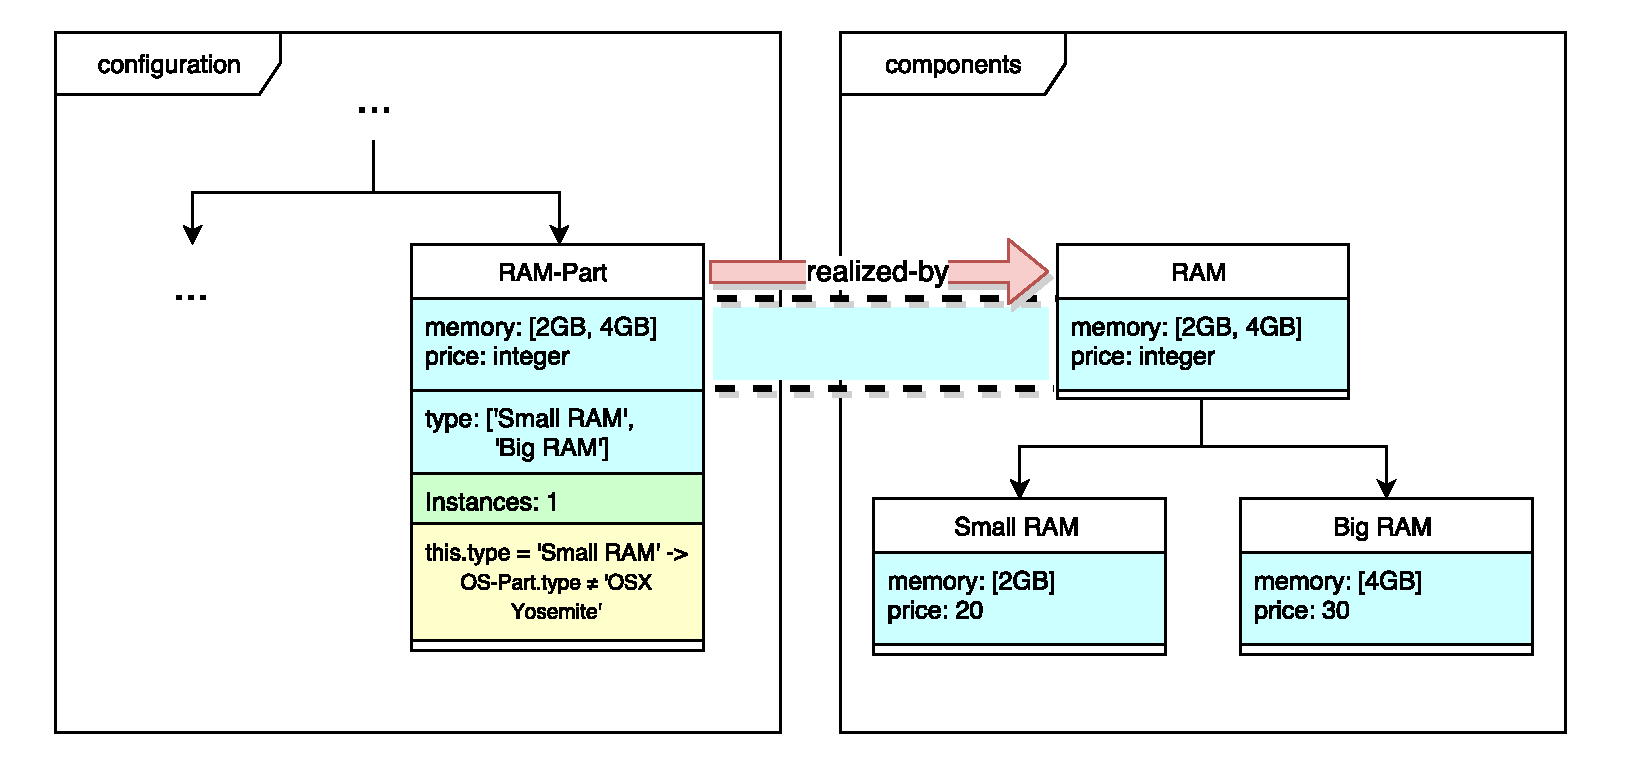
\includegraphics[width=1\linewidth]{Abbildungen/tactonModellLowLevelNotebook.pdf}
	\captionof{figure}[tactonModellLowLevelNotebook]{Part-Struktur der Notebook-Konfiguration}
	\label{fig:tactonModellLowLevelNotebook}
\end{minipage}
\vspace{1em}

Abbildung \ref{fig:tactonModellLowLevelNotebook} veranschaulicht die 'realized-by' Beziehung anhand eines Ausschnitt aus der Notebook-Konfiguration.  Der Part übernimmt die Attribute 'memory' und 'price'. Das zusätzliche Attribut 'type' kapselt beispielsweise die Information über die jeweiligen Components (z.B. Small RAM). Der Constraint veranschaulicht exemplarisch, wie die Inkompatibilität mit dem Betriebssystem vom Typ 'OSX Yosemite' formuliert werden würde.

\subsubsection{Execution}
\label{subsubsection:Execution}
Es wurde dargestellt, wie das Konfigurationswissen im Tacton Konfigurationsmodell definiert wird. Dadurch ist aber noch nicht gesagt, welche Entscheidungen ein Nutzer während der Konfiguration treffen kann. Nicht jeder Part und nicht jedes Attribut muss eine relevante Wahl darstellen. Vielleicht sollen dem Nutzer sogar Fragen auf einem anderen Abstraktionsniveau als auf Komponentenebene gestellt werden. Statt \glqq Soll eine HD oder eine SSD als Festplatte in das Notebook eingebaut werden?\grqq{} kann auch gefragt werden: \glqq Möchten Sie viel Speicherplatz oder einen schnellen Speicherzugriff?\grqq.

Der Abstimmungsprozess durch den Anwender wird unter dem Begriff \glqq Execution\grqq{} definiert. Dabei wird nicht einfach nur eine Menge an Optionen festgelegt, die dem Nutzer am Ende als Liste präsentiert werden. Stattdessen werden die Optionen hierarchisch strukturiert.

\vspace{1em}
\begin{minipage}{\linewidth}
	\centering
	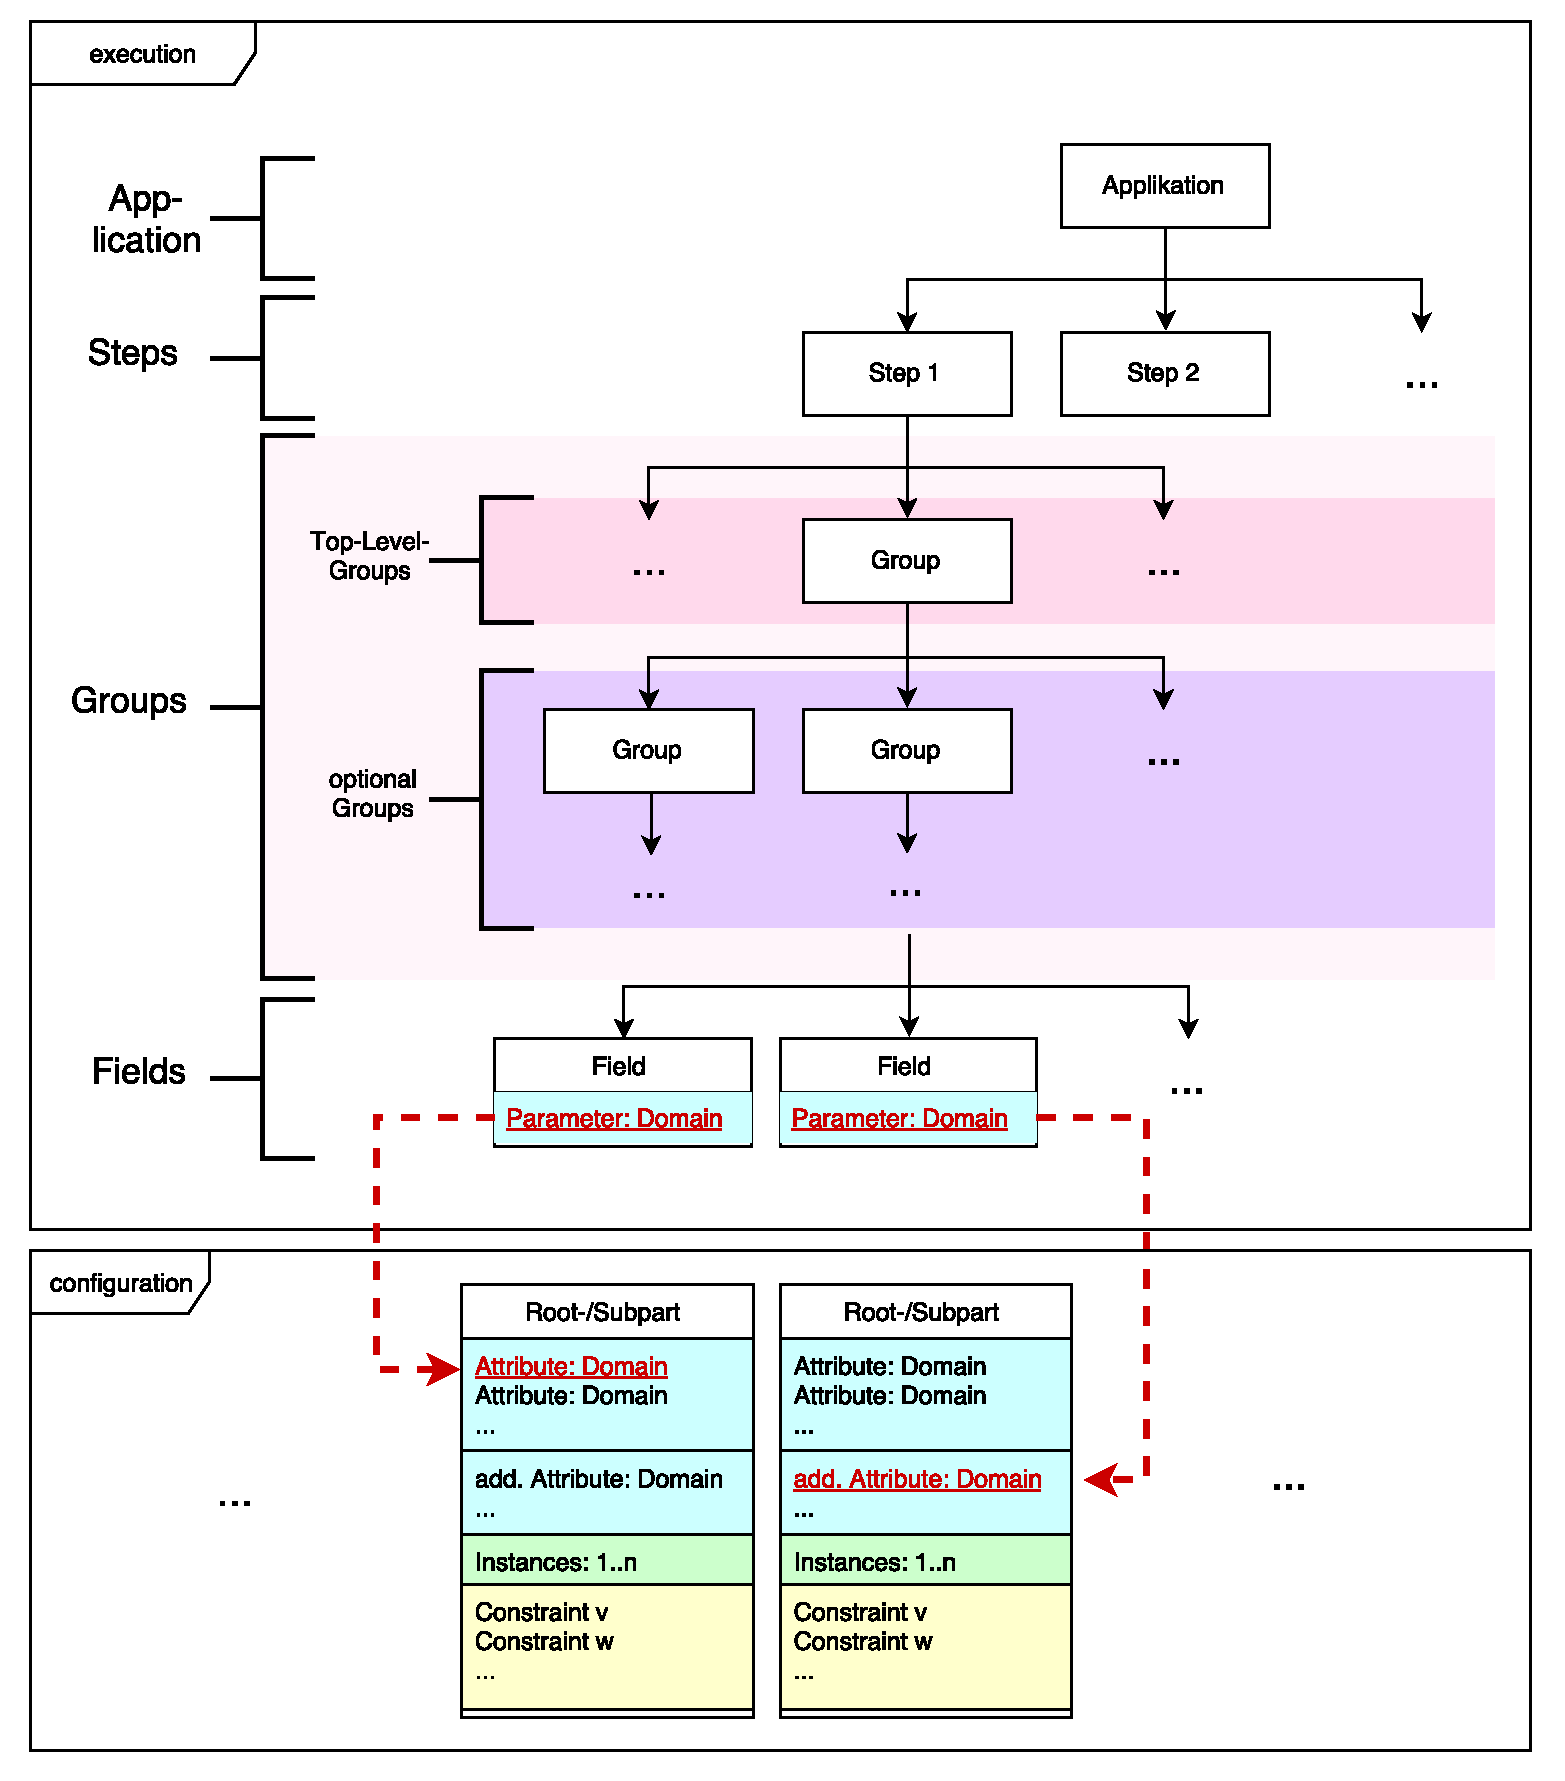
\includegraphics[width=1\linewidth]{Abbildungen/tactonModellExecution.pdf}
	\captionof{figure}[tactonModellExecution]{Generische Executionstruktur}
	\label{fig:tactonModellExecution}
\end{minipage}
\begin{minipage}{\linewidth}
	\centering
	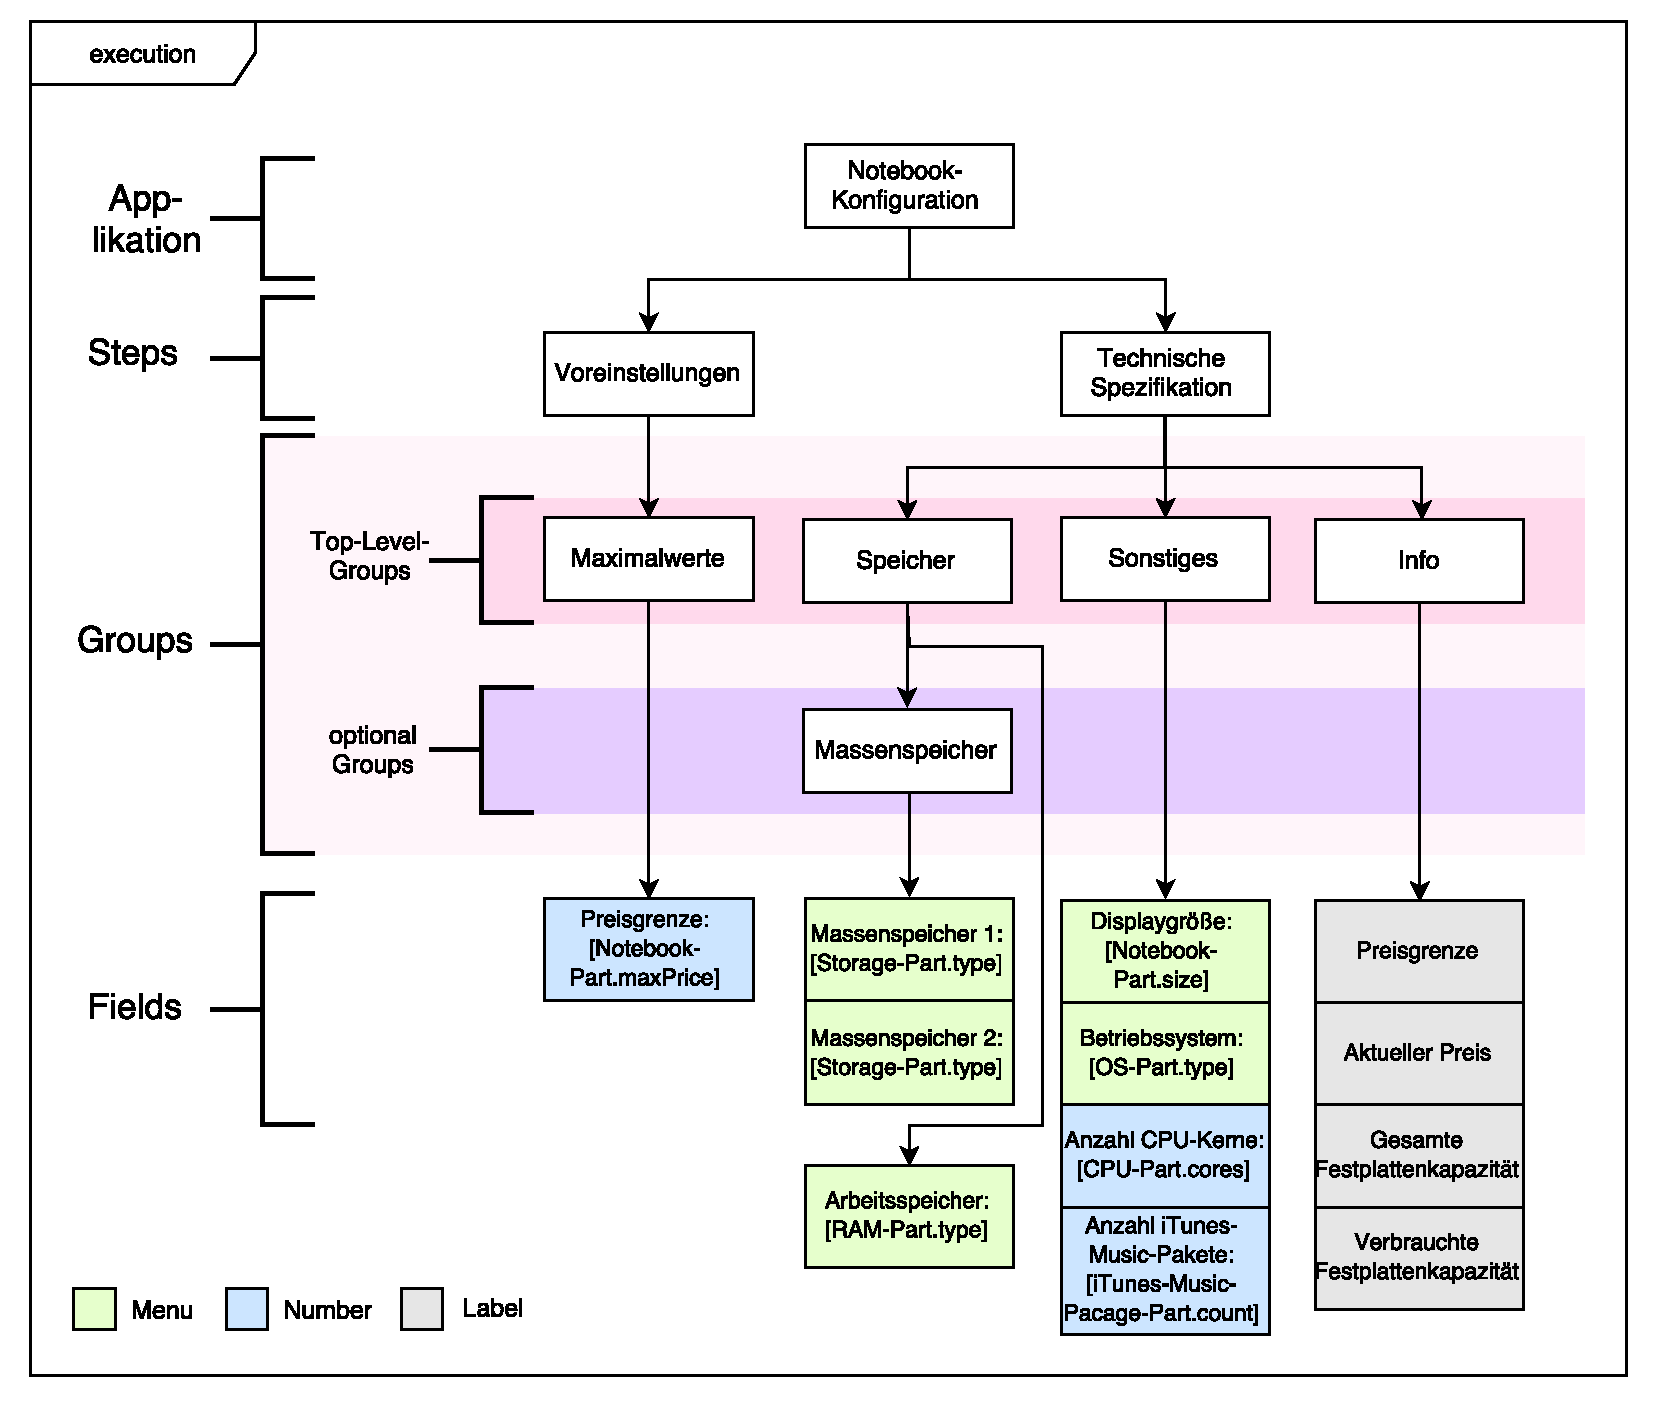
\includegraphics[width=0.8\linewidth]{Abbildungen/tactonModellExecutionNotebook.pdf}
	\captionof{figure}[tactonModellExecutionNotebook]{Exemplarische Executionstruktur einer Notebook-Konfiguration}
	\label{fig:tactonModellExecutionNotebook}
\end{minipage}
\vspace{1em}

Abbildung \ref{fig:tactonModellExecution} zeigt die generische Struktur der Execution als Baum. Abbildung \ref{fig:tactonModellExecutionNotebook} veranschaulicht das Konzept durch die exemplarische Umsetzung der Execution der Notebook-Konfiguration.
\begin{compactitem}
\item Die Wurzel wird als \textbf{Applikation} bezeichnet und kapselt den Vorgang der Konfiguration aus Anwenderperspektive.\\
Beispiel: Eine Notebook-Konfiguration.
\item Die nächste Knotenebene wird als \textbf{Steps} bezeichnet. Sie legen fest, in welcher Reihenfolge die Optionen präsentiert werden. Das ist in verschiedenen Fällen sinnvoll. Zum Beispiel dann, wenn komplexe Probleme in mehrere Schritte unterteilt oder Werte für spätere Schritte gesetzt werden sollen.\\
Beispiel: In Step 1 legt der Anwender eine Preisgrenze fest. In Schritt 2 wird die technische Spezifikation getroffen.
\item  Nun folgen $1..n$ Knotenebenen, die als \textbf{Groups} bezeichnet werden. Sie fassen Optionen zu logischen Einheiten zusammen. Die in Gruppen angeordneten Optionen müssen nicht in einer bestimmten Reihenfolge beantwortet werden.
\begin{enumerate}[(a)]
\item Die oberste Group-Ebene \textbf{Top-Level-Groups} ist obligatorisch.\\
Beispiel: Eine 'Speicher'-Group in Step 2.
\item Die Unterteilung in weitere Groups ist optional. Es kann beliebig tief geschachtelt werden.\\
Beispiel: unter 'Speicher' wird die Group 'Massenspeicher' angelegt, um sie vom 'RAM' zu unterscheiden.
\end{enumerate}
\item \textbf{Fields} sind das, womit eine Entscheidung über die Konfiguration getroffen wird. Aus Anwendersicht besteht ein Field aus einer Beschreibung und einem Interaktionselement. Eine technischer Sicht kapselt ein Field einen Parameter mit einem Wertebereich (Domain), aus welchem ein Wert (Value) gewählt wird. Die Parameter stammen aus den Attributen der Parts. Damit ist ein Parameter mit einem Part-Attribute verknüpft, wie ein Part-Attribute mit einem Features der Component Class verknüpft sind. Je nach Interaktionselement wird in unterschiedliche Feldtypen unterschieden:
\begin{enumerate}[(a)]
\item \textbf{Menu:} Wahl aus einem Wertebereich, z.B. über ein Dropdownmenü realisiert.\\
Beispiel Massenspeicher:\\
Parameter = Storage-Part.type,  Domain = ['HD', 'SSD']\\
Beispiel CPU-Kerne:\\
Parameter = CPU-Part.cores, Domain = [1..4].
\item \textbf{Number:} Eingabe eines eigenen Wertes in ein Textfeld.\\
Beispiel Preisgrenze (Eingabe in Schritt 1):\\
 Parameter = Notebook-Part.maxPrice, Domain = [integer]
\item \textbf{Label:} Anzeige eines Wertes aus Informationsgründen.\\
Beispiel Aktueller Preis (Anzeige in Schritt 2):\\
Parameter = Notebook-Part.price, Domain = [integer]
\end{enumerate}
\end{compactitem}

Die Feldtypen (a) und (b) haben gemein, dass der Anwender einen Wert aus einem Wertebereich festlegt. Bei (a) ist der Wertebereich eine Menge ausdefinierter Optionen, bei (b) ein Zahlenbereich, wobei er selbst eine Eingabe tätigt. Um die Formulierung kurz zu halten, wird das, was vom Anwender festgelegt wird, im Folgenden unter dem Begriff \glqq gewählte Option\grqq{} zusammengefasst.

Das Modell wird in einer XML-basierten Format mit der Dateiendung '.tcx' abgelegt. Die Entwicklung einer solchen Datei wird von entsprechenden Programmen unterstützt. Hierfür kann zum Beispiel \glqq TCstudio\grqq{} genutzt werden, welches eine grafische Oberfläche zur Modellentwicklung bietet \citep{tactonAbout}.

\textbf{Zwischenfazit}\\
Das Tacton-Modellierungskonzept wurde vorgestellt. Neben dem Konfigurationswissen werden darin auch die Optionen des Anwenders definiert. Diese werden durch Steps in eine Reihenfolge gebracht und durch Groups logisch gegliedert. Über Felder wählt der Anwender Optionen. Der Feldtyp Number ermöglicht die Eingabe eines eigenen Wertes. So werden Komponenten definiert, die nach Kundenanforderung konstruiert oder gefertigt werden müssen. Entsprechend der vorgestellten Produktklassifizierung in Kapitel \ref{subssubsection:Produktklassifizierung} werden so auch \ac{MTO} Produkte abgebildet.

Das Konfigurationsmodell definiert die Interaktionsstruktur. Diese muss jedoch noch in Form eine Konfigurationsoberfläche dargestellt werden. TCsite stellt eine solche Oberfläche zur Verfügung. Die Anwendung wird im folgenden analysiert.

\subsection{TCsite}
\label{subsection:TCsite}
\textbf{TCsite} ist ein webbasierter Vertriebskonfigurator. Er könnte theoretisch von Endkunden genutzt werden, bildet aber nicht die Prozesse eines eShops nach. Stattdessen handelt es sich um eine CPQ-Lösung (Configure-Price-Quote). Das bedeutet: der Anwender wird durch die Konfiguration geführt, was in einer Preiskalkulation resultiert, woraus wiederum ein Angebot erstellt wird. Eine unmittelbare Bestellung mit Zahlungsabwicklung ist nicht vorgesehen. Der Anwendungsbereich liegt also im B2B \citep{tactonAbout}.

Technisch betrachtet ist TCsite eine Webanwendung. Der serverseitige Programmcode ist in Java verfasst. Im Lieferumfang sind 'Apache Tomcat' als Application Server sowie der \textbf{TCserver} enthalten. TCserver ist das, was gemäß Kapitel \ref{subssubsection:Produktkonfiguration} als eigentlicher Konfigurator bezeichnet wird. Er beherbergt die Konfigurationsengine. Damit ist das System gemeint, welches den technischen Konfigurationsprozess durchführt \citep{tactonTCsiteHandbook}. Abbildung \ref{fig:tcsiteHighLevel} veranschaulicht die High-Level-Architektur des Standardsetups.

\vspace{1em}
\begin{minipage}{\linewidth}
	\centering
	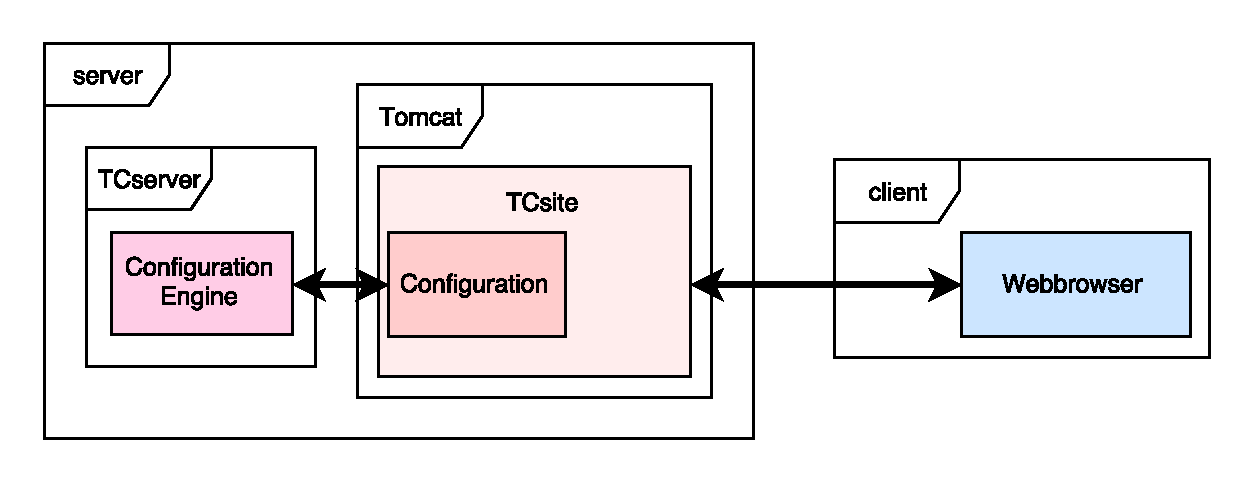
\includegraphics[width=1\linewidth]{Abbildungen/tcsiteHighLevel.pdf}
	\captionof{figure}[tcsiteHighLevel]{High-Level-Architektur von TCsite}
	\label{fig:tcsiteHighLevel}
\end{minipage}
\vspace{1em}

\subsubsection{Architektur}
\label{subsubsection:tcsiteArchitektur}

Abbildung \ref{fig:tcsiteLowLevel} visualisiert die offene Schichtenarchitektur von TCsite. Offen bedeutet, dass jede Schicht mit allen darunter liegenden Schichten kommunizieren kann. Das Fundament bildet die Persistenzschicht. Sie realisiert die Datenhaltung. Die Plattform bildet ein \ac{API} mit den Basisfunktionalitäten für die darüber liegenden Schichten. Die Module realisieren jeweils eine der drei Oberflächenbereiche der Anwendung. Außerdem bieten sie Services und Erweiterungspunkte für die oberste Schicht: die Plugins. Durch diese kann die Funktionalität von TCsite individuell erweitert werden \citep{tactonTCsiteDevelopmentManual}.

\vspace{1em}
\begin{minipage}{\linewidth}
	\centering
	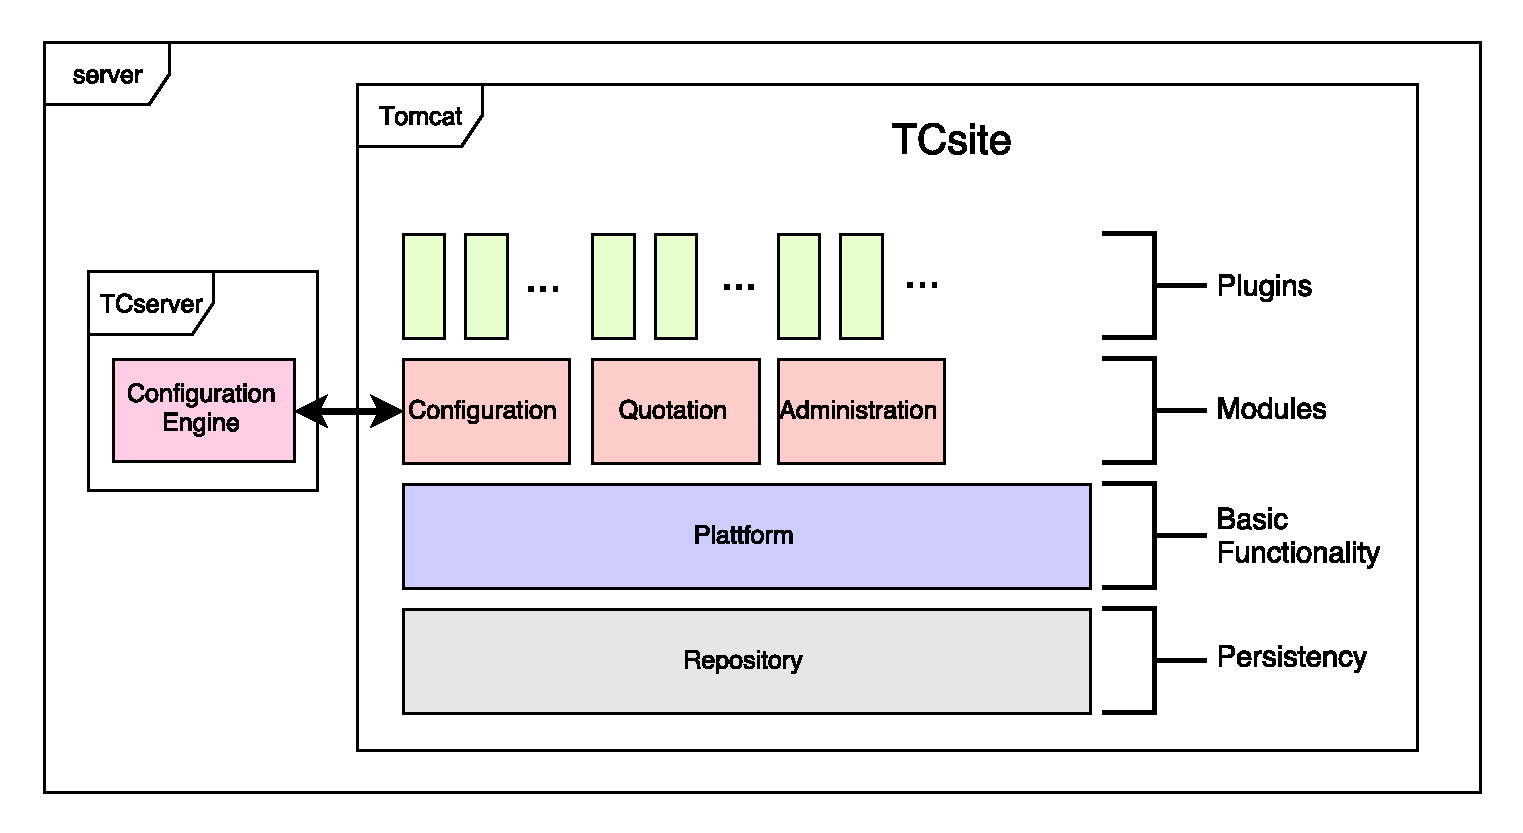
\includegraphics[width=1\linewidth]{Abbildungen/tcsiteLowLevel.pdf}
	\captionof{figure}[tcsiteLowLevel]{Schichtenarchitektur von TCsite}
	\label{fig:tcsiteLowLevel}
\end{minipage}
\vspace{1em}

Im Folgenden werden die Architekturkomponenten von unten nach oben vorgestellt.

\textbf{Repository}\\
Das Repository bietet eine Datenbank sowie ein Reihe von Funktionen zum Lesen und Schreiben der TCsite-Objekte. Das Repository ist in einen lokalen und einen globalen Speicher strukturiert. Wird ein Objekt erstellt oder geöffnet, geschieht die Bearbeitung immer auf einer Arbeitskopie in dem für jeden Nutzer spezifischen lokalen Speicher. Änderungen sind solange für andere Nutzer unsichtbar. Erst ein Commit sorgt für die nutzerübergreifende Sichtbarkeit im globalen Speicher. Bei dieser Übertragung wird eine Revisionshistorie über Objektänderungen geführt, so dass alte Zustande wieder abrufbar sind \citep{tactonTCsiteDevelopmentManual}.

\textbf{Administration}\\
Dieses Modul bildet die Administrationsoberfläche, dargestellt in Anhang \ref{app:tcsiteAdministration}. Hier werden Einstellungen getroffen und Verwaltungsaspekte realisiert. Dazu gehört zum Beispiel die Verwaltung der Nutzergruppen und Produkte.

Die Nutzergruppen definieren, welche Rechte ein TCsite-User hat. Standardmäßig verfügbar sind die Nutzergruppen \glqq Standarduser\grqq{}, \glqq Systemadministrator\grqq{} und \glqq Integrationuser\grqq{}. Letzterer Typ dient der Authentifizierung bei der Kommunikation mit externen Systemen, zum Beispiel bei einem Integrationsszenario. Bildlich personifiziert jede externe Webanfrage einen Gast, der die Maske des Integrationusers aufgesetzt und dessen Rechte bekommt.

\vspace{1em}
\begin{minipage}{\linewidth}
	\centering
	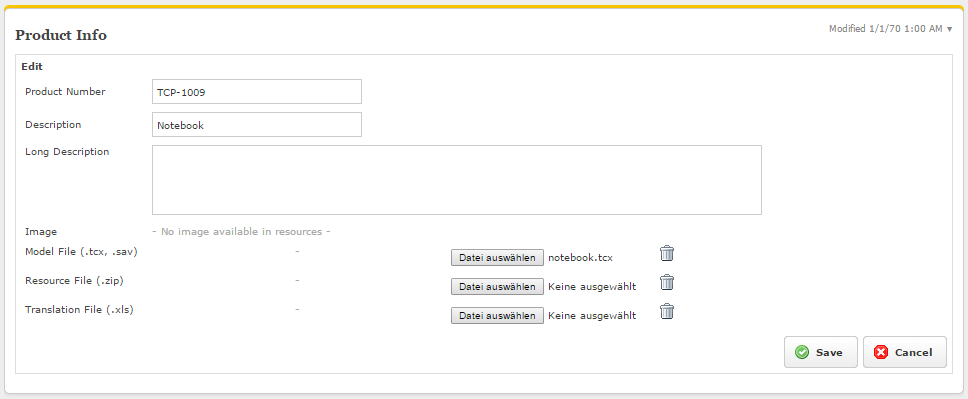
\includegraphics[width=0.6\linewidth]{Abbildungen/tcsiteAdministrationProduct.PNG}
	\captionof{figure}[tcsiteAdministrationProduct]{Detailsansicht eines Produktes aus dem Produktkatalog}
	\label{fig:tcsiteAdministrationProduct}
\end{minipage}
\vspace{1em}

Außerdem wird hier der Produktkatalog verwaltet. Abbildung \ref{fig:tcsiteAdministrationProduct} zeigt die Detailsansicht eines Produktes. Die Darstellung macht deutlich, dass neben Produktbeschreibungen auch Dateien hinterlegt werden. Wird eine Modelldatei hochgeladen, ist das Produkt konfigurierbar. Ressourcen, wie z.B. Bilder, oder eine Übersetzungsdatei können ergänzend hinzugefügt werden \citep{tactonTCsiteReferenceManual}. Entsprechend der Definition eines Konfigurationsmodells in Kapitel \ref{subssubsection:Produktkonfiguration} wird so kein bestimmtes Produkt, sondern implizit alle seine Varianten angelegt.

\textbf{Quotation}\\
Das Quotation-Modul erstellt die Quotation-View, dargestellt in Abbildung \ref{fig:tcsiteQuotationNumbered}. Technisch betrachtet realisiert das Modul Methoden für die Manipulation und Anzeige von \textbf{Quotations} sowie zur Dokumentengenerierung aus der mit ihr im Zusammenhang stehenden Daten. Aus Anwendersicht ist eine Quotation ein Angebot, dass die für ihn konfigurierten Produkte enthält. Diese werden als \textbf{QuotationItems} bezeichnet und unter 'Products' gelistet (siehe [1]) \citep{tactonTCsiteDevelopmentManual}. Betrachtet man eine Quotation als Warenkorb, sind die QuotationItems die Warenkorbpositionen. Der Vergleich hinkt insofern, als dass die Positionen eines Warenkorbs auch unabhängig von diesem als Artikel existieren. Ein QuotationItem ist jedoch eine konkrete Variante eines konfigurierbaren Produktes, die innerhalb der Quotation existiert.

\vspace{1em}
\begin{minipage}{\linewidth}
	\centering
	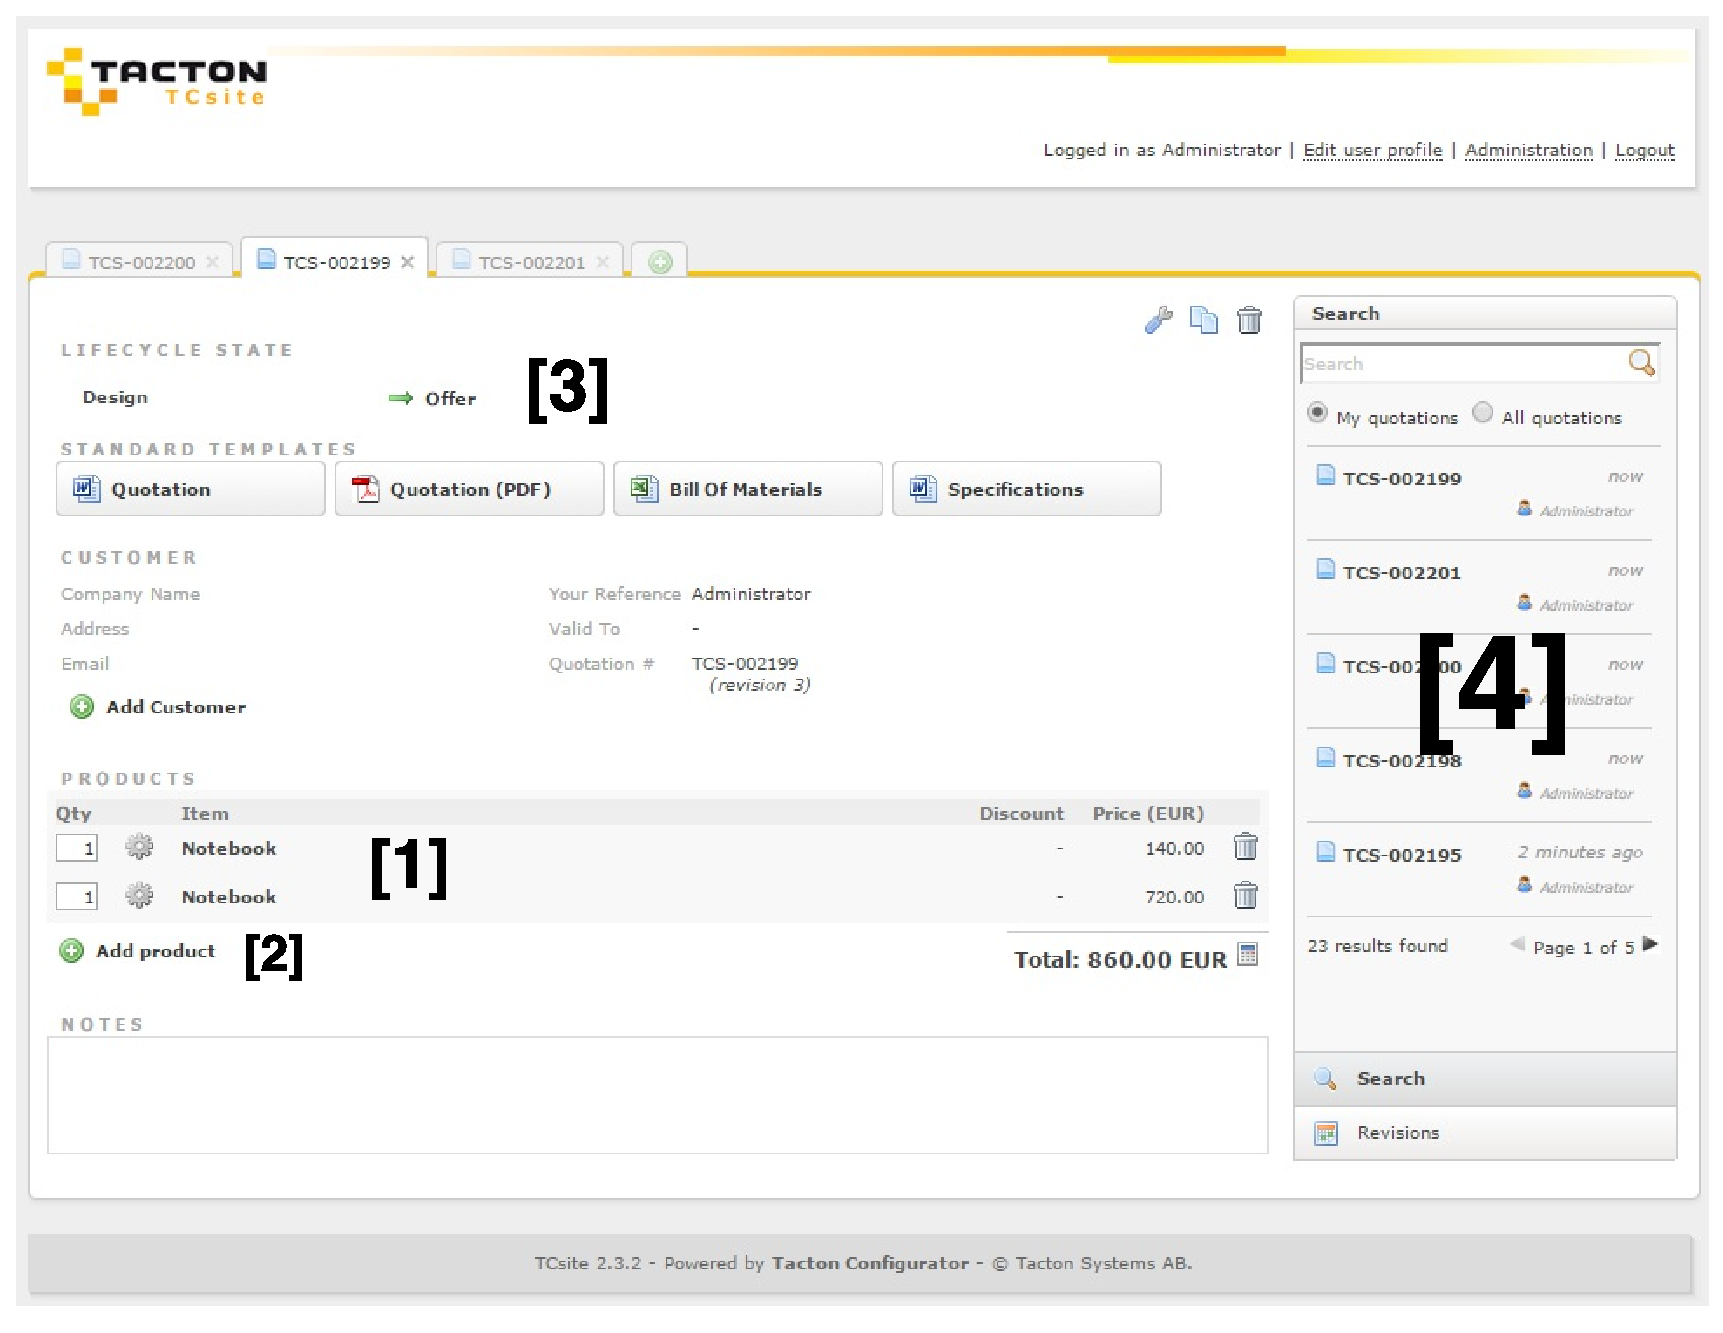
\includegraphics[width=0.7\linewidth]{Abbildungen/tcsiteQuotationNumbered.pdf}
	\captionof{figure}[tcsiteQuotationNumbered]{Quotation-View von TCsite}
	\label{fig:tcsiteQuotationNumbered}
\end{minipage}
\vspace{1em}


Der Konfigurationsprozess wird über die Schaltfläche 'Add Product' gestartet (siehe [2]). Daraufhin wählt der Anwender das gewünschte Produkt aus einer Liste aus. Im Anschluss geschieht der Übergang zum Configuration-Modul \citep{tactonTCsiteReferenceManual}.

Eine Quotation hat weiterhin einen Lebenszyklus, welcher unter 'Lifecycle State' dargestellt wird (siehe [3]). Das Angebot befindet sich zu jedem Zeitpunkt in einem bestimmten Zustand, welche über den Administrationsbereich verwaltet werden. Die Zustandsabfolge definiert den sogenannten \glqq Workflow\grqq{}. Zustände unterscheiden sich in der Sichtbarkeit für verschiedene Nutzergruppen und deren Editierbarkeit. Beispielsweise kann sich eine Quotation in den Zuständen \glqq Design\grqq{} oder \glqq Offered\grqq{} befinden. In letzterem Zustand ist nicht mehr änderbar, damit keine Inkonsistenz zum herausgegebenen Angebot entstehen kann \citep{tactonTCsiteReferenceManual}.

Die Box auf der rechten Seite stellt den Index aller Quotations dar (siehe [4]). Unter dem Suchfeld ist einstellbar, ob nur die Quotations des eingeloggten Nutzers gezeigt werden, oder ob nutzerübergreifend gelistet werden sollen. Wie im Administrationsbereich erwähnt, agieren auch externe Systeme als Nutzer, nämlich als Integrationuser. Auch Quotations, die von dieser Nutzergruppe stammen, werden hier gelistet \citep{tactonTCsiteReferenceManual}.

\textbf{Configuration}\\
Das Configuration-Modul realisiert den C-Teil des CPQ-Prozesses: die Konfiguration. Es rendert die Konfigurationsoberfläche und verwaltet die mit der Konfiguration im Zusammenhang stehenden Objekte \citep{tactonTCsiteDevelopmentManual}. Der technische Teil des Konfigurationsprozesses passiert jedoch im TCserver. Somit ist die Konfiguration als Client-Server Architektur implementiert. Das Configuration-Modul präsentiert Services, die die Kommunikation mit der Konfigurationsengine abstrahieren \citep{tactonTCsiteApiDocu}. Ansonsten ist der TCserver nicht unmittelbar ansprechbar.

\subsubsection{Konfigurationsprozess}
\label{subsubsection:tcsiteKonfigurationsprozess}

Abbildung \ref{fig:tcsiteTCserverCommunication} veranschaulicht die Kommunikation zwischen TCsite und TCserver während der Konfiguration. Das Configuration-Modul führt wiederholt zustandslose Aufrufe ('configure‘) der Konfigurationsengine durch, welche eine Antwort produziert ('result') \citep{tactonTCsiteDevelopmentManual}. Dabei weicht die Semantik von 'configure‘ und ‘result' von den Definitionen der Konfigurationsaufgabe und -lösung aus Kapitel \ref{subsubsection:begriffsuberblick} ab.

Um zu verstehen inwiefern, muss rekapituliert werden, dass interaktive Konfiguratoren einen Mechanismus zum merken des Konfigurationszustands besitzen. Ein Konfigurationszustand beinhaltet bei Tacton, welche Optionen eines Konfigurationsmodells in welchem Step gewählt wurden. Oben wurde festgestellt, dass die Aufrufe zustandslos sind. Also wird kein serverseitiger Kontext aufgebaut, der den Konfigurationszustand enthält. Die Alternative ist die Übertragung des Zustands in jedem Aufruf. Demzufolge enthält der 'configure'-Aufruf (1) das Konfigurationsmodell (2) den Konfigurationszustand und fakultativ (3) die gewählte Option des Anwenders \citep{tactonTCsiteApiDocu}. Diese Bestandteile werden ab jetzt unter dem Begriff Konfigurationsengine-Input (KE-Input) zusammengefasst. Die Antwort (\emph{result}) liefert primär den neuen Konfigurationszustand. Außerdem beinhaltet das \textbf{result} neben Informationen wie die Konfigurationslösung, dem Endpreis etc. auch die Datengrundlage zum Rendern der Konfigurationsoberfläche \citep{tactonTCsiteApiDocu}. Diese Bestandteile werden ab jetzt unter dem Begriff Konfigurationsengine-Output (KE-Output) zusammengefasst.

\vspace{1em}
\begin{minipage}{\linewidth}
	\centering
	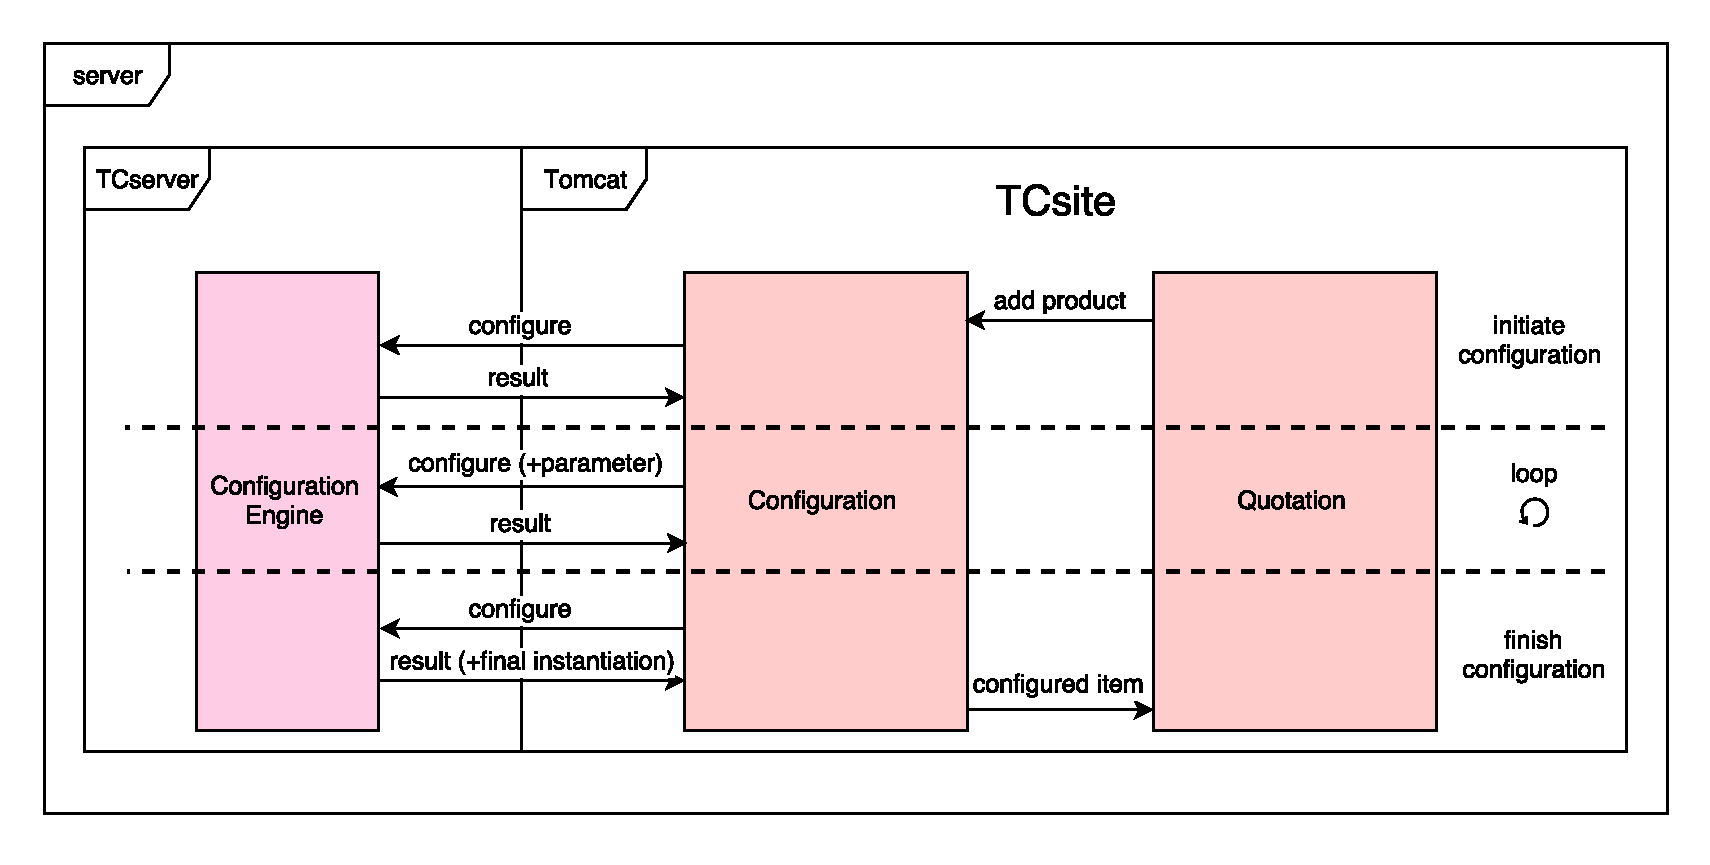
\includegraphics[width=1\linewidth]{Abbildungen/tcsiteTCserverCommunication.pdf}
	\captionof{figure}[tcsiteTCserverCommunication]{Kommunikation zwischen TCsite und TCserver}
	\label{fig:tcsiteTCserverCommunication}
\end{minipage}
\vspace{1em}

Der Konfigurationszustand und ein Verweis auf das Konfigurationsmodell, auf dass  sich dieser bezieht, werden in der Klasse \emph{configurable} zusammengefasst und persistiert. Das \emph{QuotationItem} (vorgestellt in Kapitel  \label{subsubsection:tcsiteArchitektur}) steht in einer 1-zu-1 Beziehung mit einem \emph{configurable}.

Die Kommunikation läuft in drei Phasen ab. Der erste KE-Input beinhaltet noch keine Wahl des Anwenders. Sie dient dem initialen Aufbau der Konfigurationsoberfläche entsprechend der Execution, die im Konfigurationsmodell definiert wurde. Der Konfigurationsprozess startet immer in Step 1. Die Steps müssen in der vordefinierten Reihenfolge abgearbeitet werden. Nun beginnt die Loop-Phase. Nach jeder Wahl einer Option wird die Konfigurationsengine aufgerufen und daraufhin die Oberfläche neu gerendert. Die Oberfläche spiegelt dabei den Konfigurationszustand wieder, d.h. die bisher gewählten Optionen werden hervorgehoben. Wird die Konfiguration im letzten Step vom Anwender abgeschlossen, erfolgt eine finales Aufruf der Konfigurationsengine. Aus dem KE-Output ist die Konfigurationslösung, d.h. die Variante, extrahierbar \citep{tactonTCsiteDevelopmentManual}.

Der Konfigurationsprozess wird anhand des Notebook-Beispiels aus Kapitel \ref{subsubsection:Execution} veranschaulicht. Abbildung \ref{fig:tcsiteConfigurationNumbered} zeigt die Konfigurationsoberfläche in TCsite. Die befindet sich im zweiten Step gezeigt. Mittels [1] wird zwischen den Steps gewechselt. [2] erlaubt die Navigation durch die Top-Level-Groups des aktuellen Steps. [3] stellt die Felder der aktuellen Top-Level-Group dar. Anhang \ref{app:tcSiteConfigurationOptionalGroups} zeigt anhand der 'Speicher'-Gruppe die Darstellung tieferer Group-Ebenen (siehe Kapitel \ref{subsubsection:Execution}). Außerdem wird bei [4] noch eine weitere Top-Level-Group angezeigt: die sogenannte Info-Group. Allerdings wurde bei der Execution in Kapitel \ref{subsubsection:Execution} gar keine Info-Group explizit definiert. Offensichtlich wird eine Top-Level-Group dann als Info-Group dargestellt, wenn sie nur Felder vom Typ Label enthält. Die Schlussfolgerung ist, dass die Oberfläche nicht nur präsentiert, sondern auch Darstellungslogik enthält.

\vspace{1em}
\begin{minipage}{\linewidth}
	\centering
	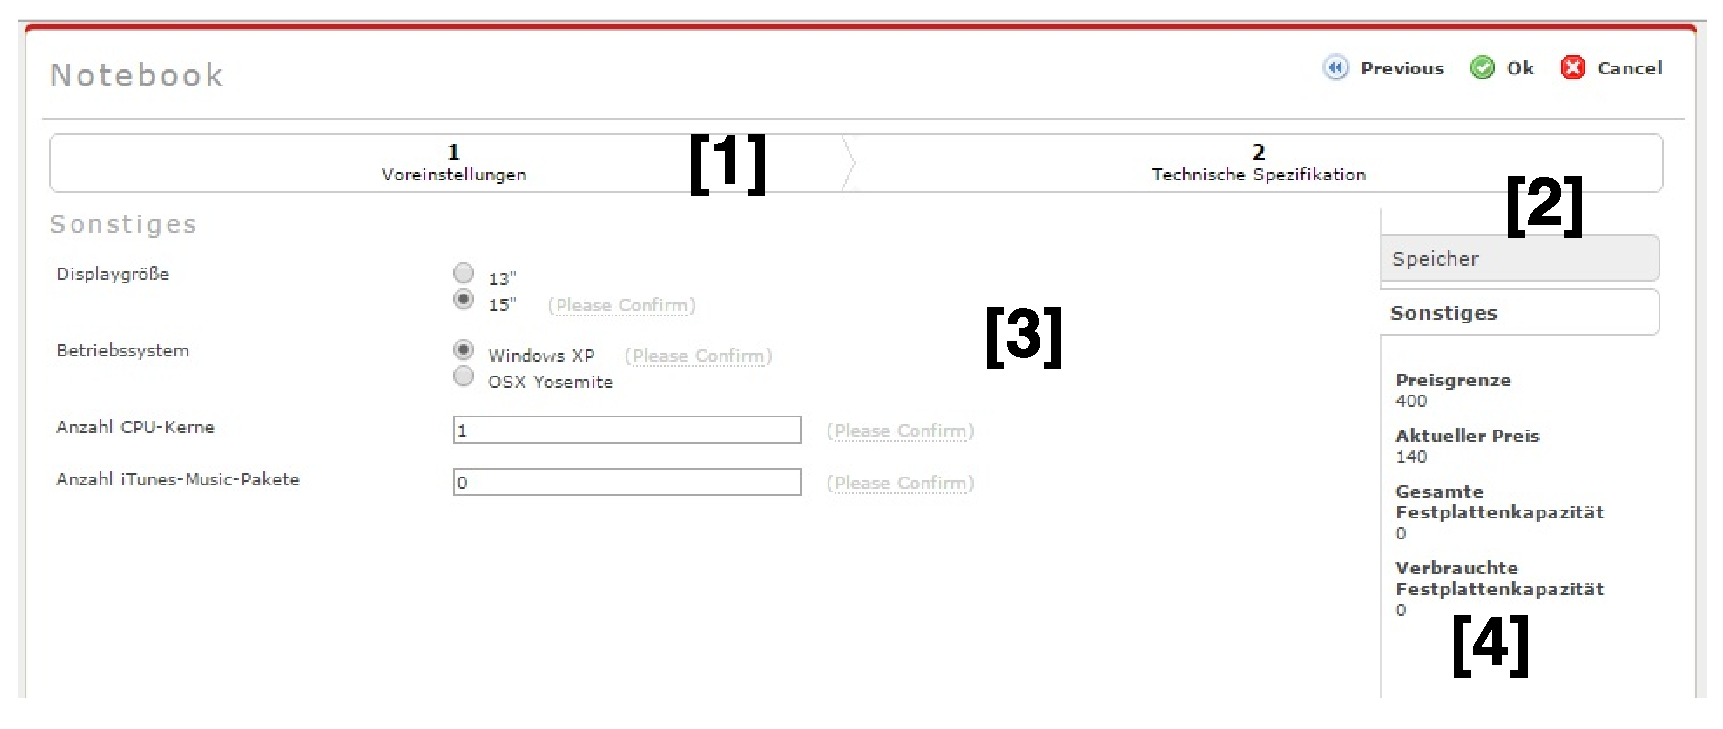
\includegraphics[width=0.8\linewidth]{Abbildungen/tcsiteConfigurationNumbered.pdf}
	\captionof{figure}[tcsiteConfigurationNumbered]{TCsite Configuration-View einer Notebook-Konfiguration}
	\label{fig:tcsiteConfigurationNumbered}
\end{minipage}
\vspace{1em}

Es fällt auf, dass bereits Optionen gewählt sind - obwohl der Anwender noch gar nichts Entschieden hat. Offensichtlich hat die Konfigurationsengine initial Default-Values gesetzt. Sie sind durch den grauen 'Please Confirm'-Hinweis gekennzeichnet.

\vspace{1em}
\begin{minipage}{\linewidth}
	\centering
	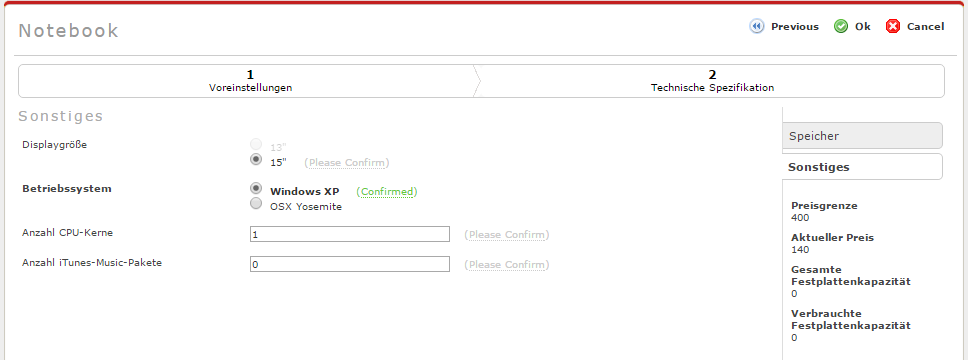
\includegraphics[width=0.8\linewidth]{Abbildungen/tcsiteConfigurationChoice.PNG}
	\captionof{figure}[tcsiteConfigurationChoice]{TCsite Configuration-View einer Notebook-Konfiguration nach Anwenderwahl}
	\label{fig:tcsiteConfigurationChoice}
\end{minipage}
\vspace{1em}

Abbildung \ref{fig:tcsiteConfigurationChoice} zeigt die Konfigurationsoberfläche, nachdem der Anwender eine Option gewählt hat (Parameter: OS.type, Value: 'Windows XP'). Die gewählte Option wird \glqq unverhandelbar\grqq{}. Das wird gekennzeichnet durch das grüne 'Confirmed'. Außerdem wird überprüft, wie die gewählte Option die anderen verfügbaren Optionen beeinflusst. Was zu einem Konflikt führt, wird ausgegraut. Beim Feld 'Displaygröße' ist zu beobachten, dass die Wahl der Konfigurationsengine von '13' auf '15' geändert wurde. Offensichtlich sind Werte, die nicht vom Anwender gesetzt wurden, \glqq verhandelbar\grqq{}. Die Konfigurationsengine sorgt folglich immer für einen konfliktfreien Zustand. Durch einen Klick auf 'Confirm' bzw. 'Please Confirm' können Optionen zwischen verhandelbar und unverhandelbar gewechselt werden.

\vspace{1em}
\begin{minipage}{\linewidth}
	\centering
	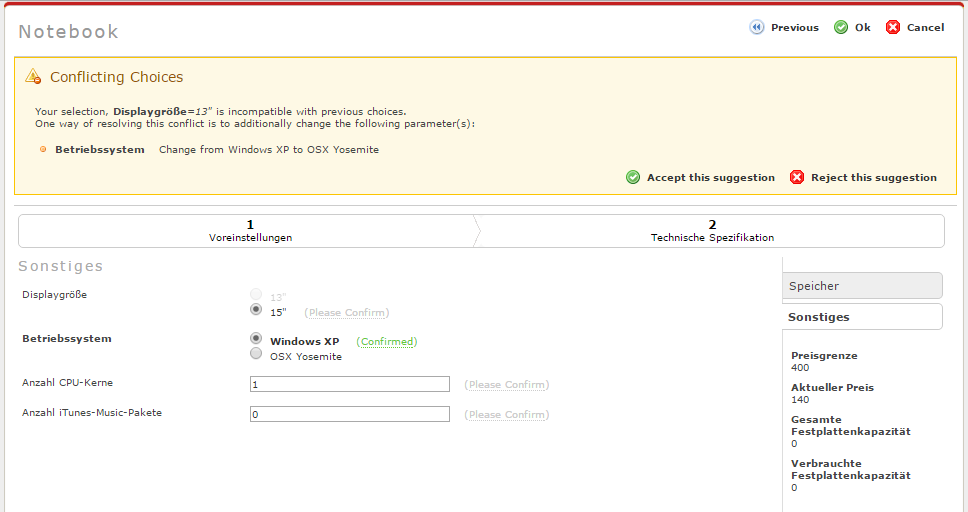
\includegraphics[width=0.8\linewidth]{Abbildungen/tcsiteConfigurationConflict.PNG}
	\captionof{figure}[tcsiteConfigurationConflict]{TCsite Configuration-View in einer Konfliktsituation}
	\label{fig:tcsiteConfigurationConflict}
\end{minipage}
\vspace{1em}

Ausgegraute Optionen sind dennoch wählbar. Abbildung \ref{fig:tcsiteConfigurationConflict} zeigt die Konfigurationsoberfläche nach einem Klick auf die Displaygröße '13'. Dennoch ist '15' immer noch die aktive Option. Gleichzeitig wird am oberen Ende eine Konflikthinweis angezeigt. Die Konfigurationsengine weist darauf hin, dass Optionen im Widerspruch stehen und schlägt eine Konfliktlösung vor. Diese kann angenommen oder abgelehnt werden. Im letzteren Fall bleibt die Konfiguration einfach in dem Zustand vor der Wahl der konfliktverursachenden Option. Auch die Eingabe von Werten in ein Textfeld kann zu Konflikten führen. Beispielsweise dann, wenn diese außerhalb der Domain des Parameters liegen oder im Widerspruch mit einer anderen Wahl stehen. 

Wird der Konfigurationsprozess über die Schaltfläche 'Ok' beendet, kehrt TCsite zum Quotation Modul zurück. Dort erscheint die Variante in der Liste der QuotationItems.

\subsubsection{Erweiterbarkeit}
\label{subsubsection:Erweiterbarkeit}

Zur Erweiterung der Funktionalität bietet TCsite ein Pluginkonzept, welches Abbildung \ref{fig:tcsiteLowLevelExtensions} visualisiert. Neben den oben diskutierten Verantwortlichkeiten definieren die Plattform und die Module sogenannte Extensionpoints \citep{tactonTCsiteApiDocu}. Extensionpoints sind das, was in anderen Erweiterungskonzepten als Events bezeichnet wird: Ereignisse im Kontrollfluss der Geschäftsprozesse. Plugins können Methoden bereitstellen, die an den entsprechenden Ereignisstellen aufgerufen werden  \citep{tactonTCsiteDevelopmentManual}.

\vspace{1em}
\begin{minipage}{\linewidth}
	\centering
	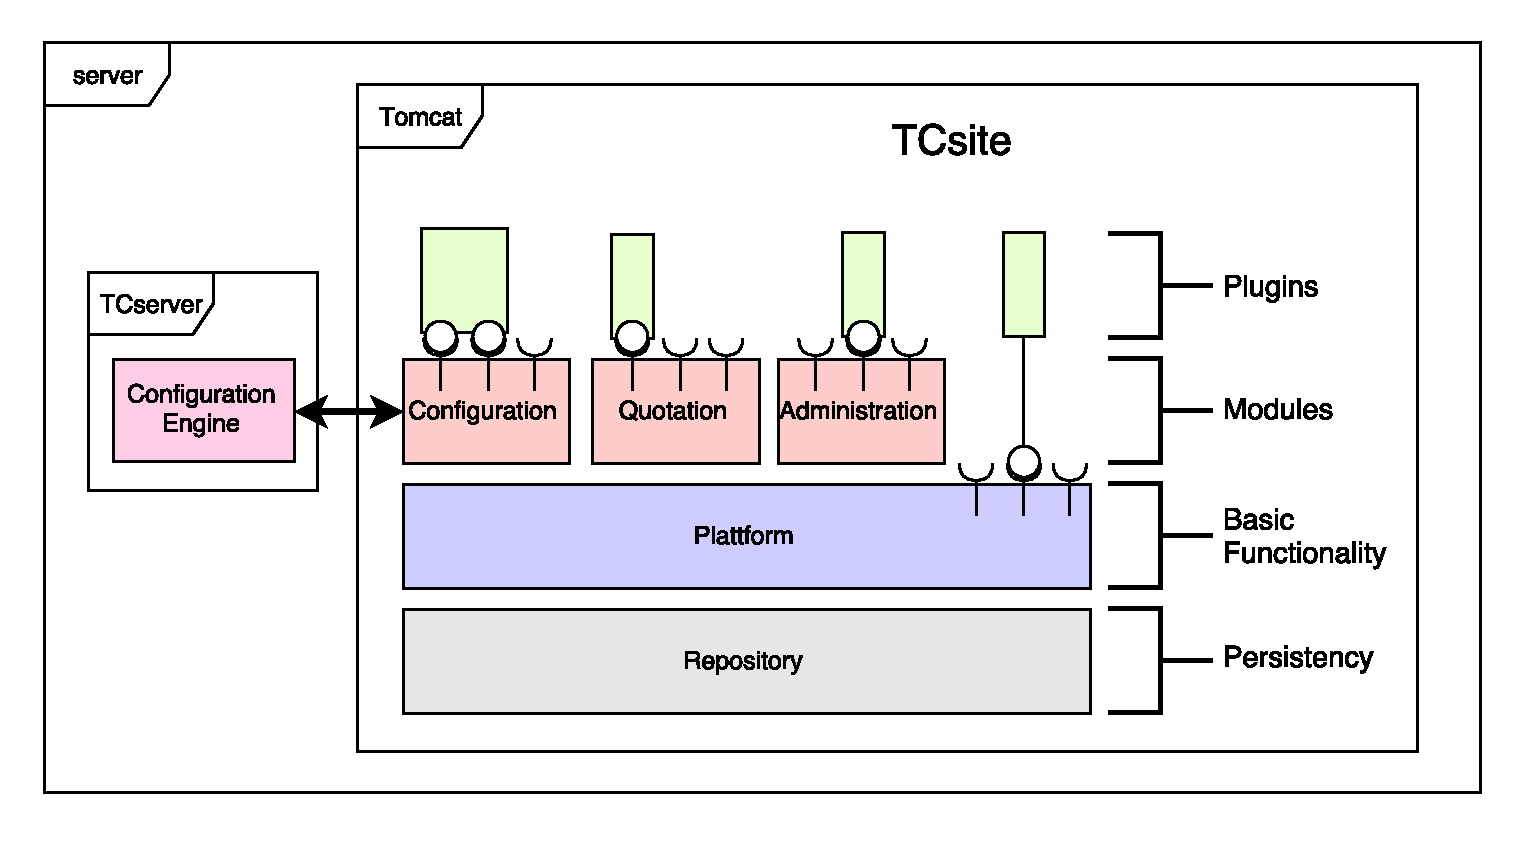
\includegraphics[width=0.8\linewidth]{Abbildungen/tcsiteLowLevelExtensions.pdf}
	\captionof{figure}[tcsiteLowLevelExtensions]{TCsite Pluginkonzept}
	\label{fig:tcsiteLowLevelExtensions}
\end{minipage}
\vspace{1em}

Jedes Plugin hat Zugriff auf das Repository, die Plattform und das Moduls, zu dem es gehört. Die Plattform stellt außerdem ein paar spezielle Erweiterungspunkte bereit. Sie erlaubt unter anderem die Definition von Webcontrollern. Das bedeutet: Methoden, die auf HTTP-Requests an bestimmte URIs innerhalb des TCsite-Addressraums reagieren.

\textbf{Zusammenfassung}\\
Der Produktkatalog von TCsite besteht nicht aus explizit ausdefinierten Varianten, sondern Produkten mit Konfigurationsmodellen. Erst innerhalb einer \emph{Quotation} werden kundenspezifische Varianten durch einen Konfigurationsprozess generiert, welche als \emph{QuotationItems} bezeichnet werden. Der Konfigurationsprozess ist die Führung des Anwenders durch die in einem Konfigurationsmodell definierte \emph{execution}, bei dem in jedem Step Optionen gewählt werden. Alle gewählten Optionen eines Konfigurationsmodells sind dessen Konfigurationszustand. Die Einheit aus Konfigurationsmodell und Konfigurationszustand wird als \emph{configurable} persistiert und mit dem \emph{QuotationItem} verbunden.

Der Konfigurationsprozess passiert im Configuration-Modul. Technisch betrachtet werden dabei \emph{KE-Inputs} verarbeitet, die mit \emph{KE-Outputs} beantwortet werden. Ein KE-Input besteht aus dem Konfigurationsmodell, dessen Konfigurationszustand und (fakultativ) der gewählten Option des Anwenders. Das Konfigurationsmodell und der Konfigurationszustand stammen aus dem \emph{configurable}, die gewählte Option des Anwenders wird über die Konfigurationsoberfläche erhoben. Die Konfigurationsoberfläche wird aus den Daten des \emph{KE-Outputs} erstellt.

\subsubsection{Zwischenfazit}
\label{subsubsection:tcsiteFazit}

Die Daten aus dem KE-Output können auch einem externen System zum Aufbau einer Konfigurationsoberfläche zur Verfügung gestellt werden. Über die Oberfläche wählt der Anwender Optionen, die an TCsite zurückgegeben werden. Dort wird in Verbindung mit dem entsprechenden \emph{configurable} ein KE-Input definiert. Über den KE-Output kann die Konfigurationsoberfläche im externen System wiederum aktualisiert werden und der Prozess beginnt von neuem. Die für diesen Vorgang relevanten Informationen müssen nur irgendwie zwischen dem externen System und TCsite transportiert werden. Das Pluginkonzept erlaubt die Definition von Serviceendpunkten über Webcontroller. An diesen können HTTP-Requests ausgewertet und beantwortet werden. Dadurch ist es möglich, einen Webservice zu implementieren, der eine Schnittstelle für externe Konfigurationsoberflächen bereitstellt.

Potentieller Client dieses Services ist jedes System, welches HTTP nutzen kann. Das trifft auf jede Webanwendung zu. eShops-Systeme sind per se Webanwendungen. Somit können technische Bedingungen an das eShop-System für das Integrationsszenario formuliert werden: (1) das System muss modifizierbar sein, (2) die Modifizierung muss einen Webservice in einer Client-Server Architektur nutzen können und (3) die Verwaltung von Varianten muss integraler Bestandteil des Systems sein.

??????????Jedes Shopsystem, welches diese technischen Bedingungen erfüllt, kommt für das Integrationsszenario in Frage. Ein interner Evaluierungsprozess der Lino GmbH, bei dem zusätzlich ökonomische Faktoren bewertet wurden, hat zu Shopware als System für die prototypische Entwicklung geführt.??????

\subsection{Shopsystem}
\label{subsection:Shopsystem}

Shopware wird von der shopware AG in Schöppingen entwickelt. Das eShop-System ist aus einer Individuallösung gewachsen, welche 2003 von den heutigen Geschäftsführern entwickelt wurde. Infolgedessen wurde das Unternehmen 2008 als Vertriebsgesellschaft für die Software gegründet. Aktuell liegt die fünfte Version vor. Shopware wird in einem Dual-License Modell vertrieben. Die Community Edition wird unter der \citeauthor{gnuAGPLv3} Open-Source Lizenz \glqq AGPLv3\grqq{} angeboten. Außerdem existieren drei kommerzielle Versionen \citep{shopwareUnternehmen}.

Im Folgenden wird Shopware einer technischen Analyse unterzogen. Darauf aufbauend wird die Erweiterbarkeit des Systems besprochen. Anschließend wird diskutiert, wie die Produktkonfiguration in der Standardinstallation technisch realisiert wird. Daraus kann eine Abgrenzung zum Tacton-Produktkonfigurator gewonnen und gleichzeitig dessen Integration motiviert werden. Die abschließende Betrachtung der Konfiguration im Einkaufsprozess liefert Ansatzpunkte für das Integrationskonzept.

\subsubsection{Architektur}
\label{subsubsection:shopwareArchitektur}
Shopware basiert auf der Programmiersprache PHP und verwendet eine relationale MySQL Datenbank. Grundlage des Technologiestacks ist das Zend-Framework, welches in der eigenentwickelten Abwandlung namens Enlight vorliegt \citep{shopware5Docs}.

Die Shopware-Architektur implementiert das \ac{MVC}-Muster, dargestellt in Abbildung \ref{fig:shopwareMVC}. Das \textbf{Model} definiert die Datenstrukturen des Systems (z.B. Artikel, Kategorien, Bestellungen etc.). Doctrine wird für die \ac{ORM} verwendet. Dadurch wird eine Abstraktionsschicht über die Datenbank aufgebaut \citep{shopware5Docs}. Das Framework ermöglicht die zentrale Definition der Datenbankstruktur in PHP und einen objektorientierten Datenzugriff \citep{shopware4Docs}.

\vspace{1em}
\begin{minipage}{\linewidth}
	\centering
	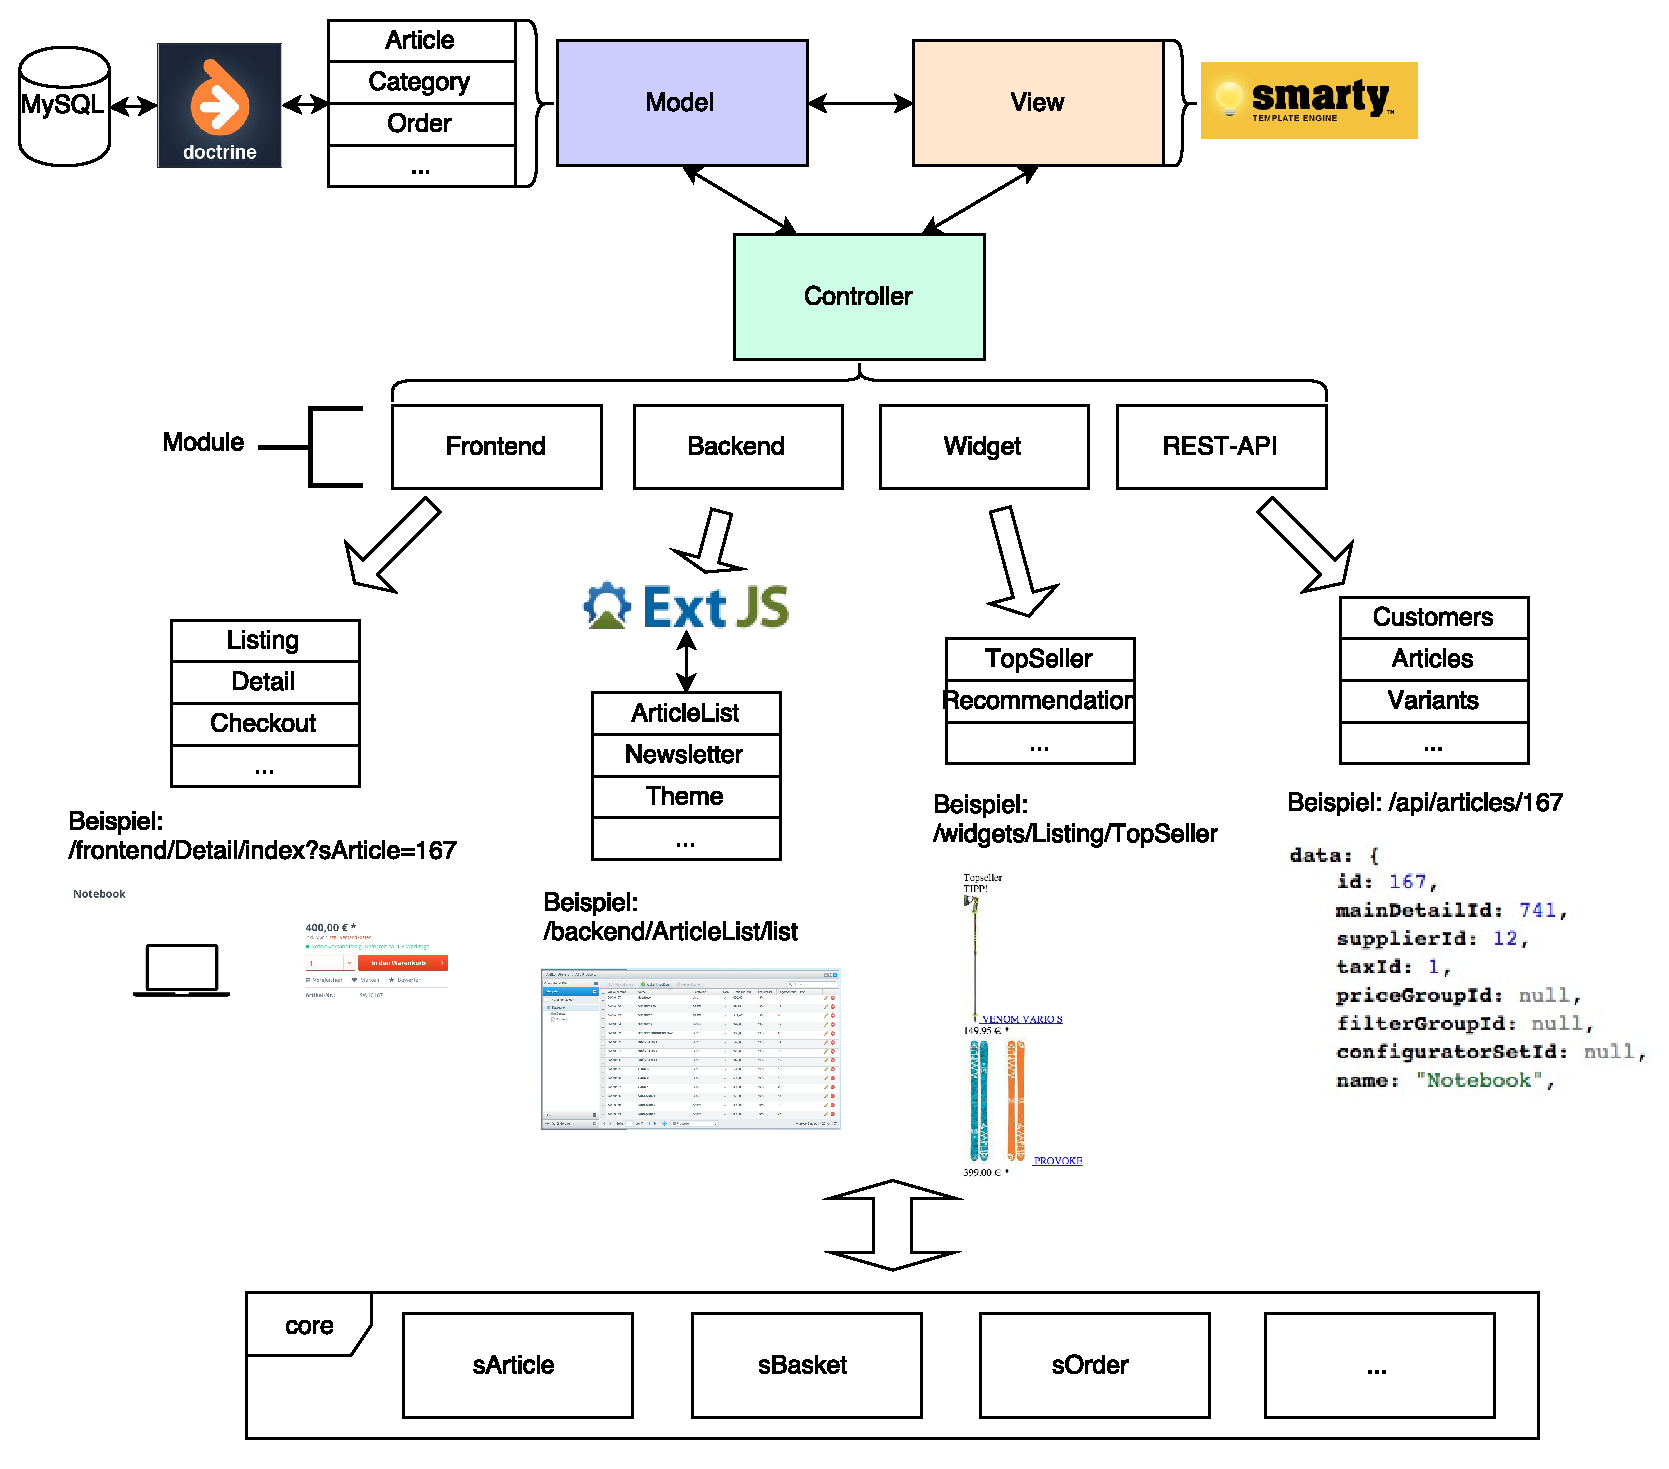
\includegraphics[width=1\linewidth]{Abbildungen/shopwareMVC.pdf}
	\captionof{figure}[shopwareMVC]{Shopware High-Level-Architektur}
	\label{fig:shopwareMVC}
\end{minipage}
\vspace{1em}

Die \textbf{View} nutzt die Templating-Engine Smarty. Diese erweitert den HTML-Syntax um spezielle Smarty-Tags. Sie ermöglichen unter anderem die Definition von Variablen zur Darstellung von Daten aus dem Model. Außerdem können über Smarty-Tags sogenannte Blöcke definiert werden. Es handelt sich hierbei um addressierbare Bereiche innerhalb eines Templates, die das Markup strukturieren. Sie spielen eine Rolle für das Erweiterungskonzept \citep{shopware5Docs}.

Controller sind Klassen, die Webrequests entgegen nehmen und eine Präsentation der Antwort durch Vermittlung zwischen Model und View entwickeln. Sie bieten Methoden an, welche als Actions bezeichnet werden. Diese sind die bestimmten URIs zugeordnet. Controller sind nach Verantwortungsbereichen aufgeteilt. Diese werden als Module bezeichnet und folgendermaßen typisiert \citep{shopware4Docs}:
\begin{compactitem}
\item \textbf{Frontend}-Controller sind für die Storefront zuständig. Das bedeutet: alle Seiten, die ein Kunde sieht.\\
Beispiele: Artikelliste einer bestimmten Kategorie, Detailseite eines Artikels, Warenkorb, Nutzeraccount, ...
\item \textbf{Widget}-Controller generieren wiederverwendbare Bestandteile der Storefront.\\
Beispiel: Liste der meistverkauften Artikel.
\item \textbf{Backend}-Controller sind für die Datenverwaltung der Shopadministration zuständig. Sie generieren jedoch keine Einzelseiten wie im Falle der Frontend-Controller. Stattdessen ist der administrative Bereich als Single-Page-Application mittels des Javascript-Frameworks Ext JS implementiert. Dieses stellt eine Menge an Steuerelementen (z.B. Menüs, Formulare, etc.) zur Verfügung.\\
Beispiele: Nutzerverwaltung, Artikelverwaltung, Pluginverwaltung, ...
\item Für externe Systeme, die mit den Ressourcen von Shopware interagieren möchten, ist eine \textbf{REST-API} implementiert. Ein vollständige Übersicht aller Ressourcenendpunkte ist \citep{shopwareRestApiEndpunkte} zu entnehmen.\\
Beispiel: Abrufen des Artikels mit der ID 167.
\end{compactitem}

Der Großteil der Logik ist jedoch nicht in den Actions, sondern den sogenannten core-Klassen implementiert \citep{shopware4Docs}. Beispielsweise wird der Request zum Hinzufügen einer Warenkorbposition vom Checkout-Controller entgegen genommen, die notwendigen Geschäftsprozesse finden aber in der Serviceklasse 'sBasket' statt.

\subsubsection{Erweiterbarkeit}
\label{subsubsection:shopwareErweiterbarkeit}
Der Quellcode der Community-Edition liegt offen. Theoretisch ist eine Erweiterung der Funktionalität über ein direktes Eingreifen in den Shopware-Kern denkbar. Der Hersteller sieht jedoch eine Anpassung über Plugins vor. Entsprechend der \ac{MVC}-Architektur wird in logische (Controller), Daten- (Model) und Template- (View) Erweiterungen unterschieden \citep{shopware5Docs}.

\textbf{Logische Erweiterungen}\\
Logische Erweiterungen werden über Events und Hooks realisiert. Events sind \glqq definierte Ereignisse, die im Workflow des Shops auftreten\grqq{} \citep{shopware4Docs}. Plugins können Code registrieren, welcher an den Ereignispunkten ausgeführt wird. Steht kein Event für die geplante Modifikation zur Verfügung, kann Plugin-Code über das Hooksystem unmittelbar auf Funktionen des Shopware-Kerns registriert werden \citep{shopware5Docs}. Damit ist das Erweiterungskonzept flexibler als das von TCsite.

Events werden in Controller-Events und Notify-Events unterschieden \citep{shopware4Docs}. \textbf{Controller-Events} sind an den Dispatch-Vorgang gekoppelt. Der shopware-Entwickler \citet{noegel15Diaspatch} definiert Dispatching als einen Prozess, bei dem das Resquest-Objekt gehandhabt, daraus das relevante Modul, der Controller und die Action extrahiert, der entsprechende Controller instanziiert und dieser zur Behandlung des Request gebracht wird. Leitet ein Controller den Request zu einem anderen Controller weiter, wiederholt sich dieser Vorgang. Plugins können auszuführenden Code registrieren, der vor (\textbf{PreDispatch}) oder nach dem Dispatching (\textbf{PostDispatch}) ausgeführt werden soll. Außerdem können sie den Dispatch-Prozess auf eigene Funktionen umleiten und so ganze Controller-Methoden ersetzen. \textbf{Notify-Events} entsprechen hingegen den in Kapitel \ref{subsubsection:Erweiterbarkeit} erwähnten Extension-Points von TCsite. Sie finden beispielsweise in den Core-Klassen Verwendung. So kann abseits der Controller in den Programmablauf eingegriffen werden \citep{shopware4Docs}.

Hooks bieten einen generischeren Ansatz. Events sind auf den Dispatchprozess und alle sonstigen Punkte beschränkt, an denen ein Shopware-Entwickler Erweiterbarkeit vorgedacht hat. Das Hooksystem bezeichnet die Möglichkeit, jede public und protected-Funktion von Shopware zu Erweitern. Sie erlauben die Modifizierung der Eingangsparameter und Rückgabewerte der Originalfunktion sowie deren komplette Ersetzung \citet{noegel15Hooks}.

\textbf{Daten-Erweiterungen}\\
Im Gegensatz zu TCsite erlaubt Shopware die Erstellung und Modifizierung von Datenbanktabellen. Sollen bestehende Datenmodelle nur um bestimmte Eigenschaften ergänzt werden, existiert das Attributsystem. Gewisse Shopware-Entitäten (z.B. s\_user für Shopkunden) haben Attributtabellen (z.B. s\_user\_attributes) in einer 1-zu-1 Beziehung zugeordnet. Plugins können diesen beliebige Spalten hinzufügen (z.B. die Lieblingsfarbe des Kunden) \citep{shopware5Docs}.

\textbf{Template-Erweiterungen}\\
Die View bietet Erweiterungspunkte über das Smarty-Block-System. Die Blöcke können durch eigenen Templatecode ersetzt oder erweitert werden. Weiterführend sind so eigene CSS- und Javascriptdateien im Seitenkopf einbindbar. Folglich kann durch Template-Erweiterungen auch clientseitige Logik implementiert werden.

Abschließend wird bemerkt, dass Oberflächenerweiterungen im administrativen Bereich nicht durch Smarty realisiert werden, sondern durch das dort eingesetzte Framework \emph{Ext JS}. Dies wird nicht in der offiziellen Dokumentation erwähnt. Stattdessen weisen die Orientierungsbeispiele für Backenderweiterungen implizit darauf hin (siehe \citet{shopwareBackendPluginExamples}). \emph{Ext JS}-Erweiterungen sind ein komplexer Sachverhalt und werden in dieser Arbeit nicht weiter behandelt.

\subsubsection{Konfiguration}
\label{subsubsection:shopwareKonfiguration}
Shopware behauptet in der der offiziellen Funktionsübersicht, bereits in der Standardinstallation einen Konfigurator zu besitzen \citep{shopware5Funktionsuebersicht}. Im Folgenden wird dessen Implementierung analysiert. Daraufhin wird dessen Integration in den Einkaufsvorgangs diskutiert.

\textbf{Technische Analyse}\\
Ein Artikel, den ein Kunde kaufen kann, wird über den entsprechenden Menüpunkt im Backend angelegt (siehe Abbildung \ref{app:shopwareBackendArtikel}). Über das Userinterface kann dieser als \glqq Varianten-Artikel\grqq{} gekennzeichnet werden. Dadurch wird der Variantenreiter aktiviert, unter dem der Administrator alle Varianten des Artikels festlegt.

Dazu werden sogenannte \glqq Gruppen\grqq{} (z.B. 'Storage') angelegt, die wiederum \glqq Optionen\grqq{} (z.B. 'HDD' oder 'SSD') besitzen. Das ist äquivalent zu den Begriffen \glqq Parameter\grqq{} und \glqq Domain\grqq{} in der Execution des Tacton-Konfigurationsmodells, vorgestellt in Kapitel \ref{subsubsection:Execution}. Es werden also die Wahlmöglichkeiten des Anwenders definiert, jedoch ohne Konfigurationswissen. Die Gruppen und Optionen werden separat in der Datenbank gespeichert und sind Artikelübergreifend verwendbar. Über den Button \glqq Varianten generieren\grqq{} (siehe Abbildung \ref{app:shopwareBackendArtikelVarianten}) werden alle Varianten explizit in der Datenbank angelegt, die sich aus der Kombination der Optionen ergeben. Übertragen auf Notebook-Beispiel ergibt das folgende Rechnung:

$3_{Massenspeicher1}*3_{Massenspeicher2}*2_{Arbeitsspeicher}*2_{Displaygr"o"se}*2_{Betriebssystem}*4_{Anzahl CPU-Kerne}*99_{Anzahl iTunes-Music-Pakete} = 28512  Varianten$

Damit passiert das, was durch das Konfigurationsmodell laut Kapitel \ref{subsubsection:begriffsuberblick} verhindert werden soll: das explizite definieren und abspeichern aller Varianten. Es gibt keine Constraints. Dementsprechend muss der Administrator händisch alle inkorrekte Varianten löschen und die Preise der korrekten Varianten eintragen. Die in Kapitel \ref{subsubsection:begriffsuberblick} vorgestellte Konfigurationsdefinition \citet{sabin98} fordert aber Constraints. Somit stellt Shopware keine Konfigurationsprozess bereit, sondern die Selektion einer explizit definierten Variante entsprechend der gewählten Optionen des Anwenders aus einer Datenbank.

\textbf{Einkaufsvorgang}\\
Ausgehend von dieser Analyse ist der Einkaufsvorgang eines Varianten-Artikels unter Berücksichtigung der technischen Prozesse als Aktivitätsdiagramm in Abbildung \ref{fig:shopwareKonfigurationFlussdiagramm} darstellbar .

\vspace{1em}
\begin{minipage}{\linewidth}
	\centering
	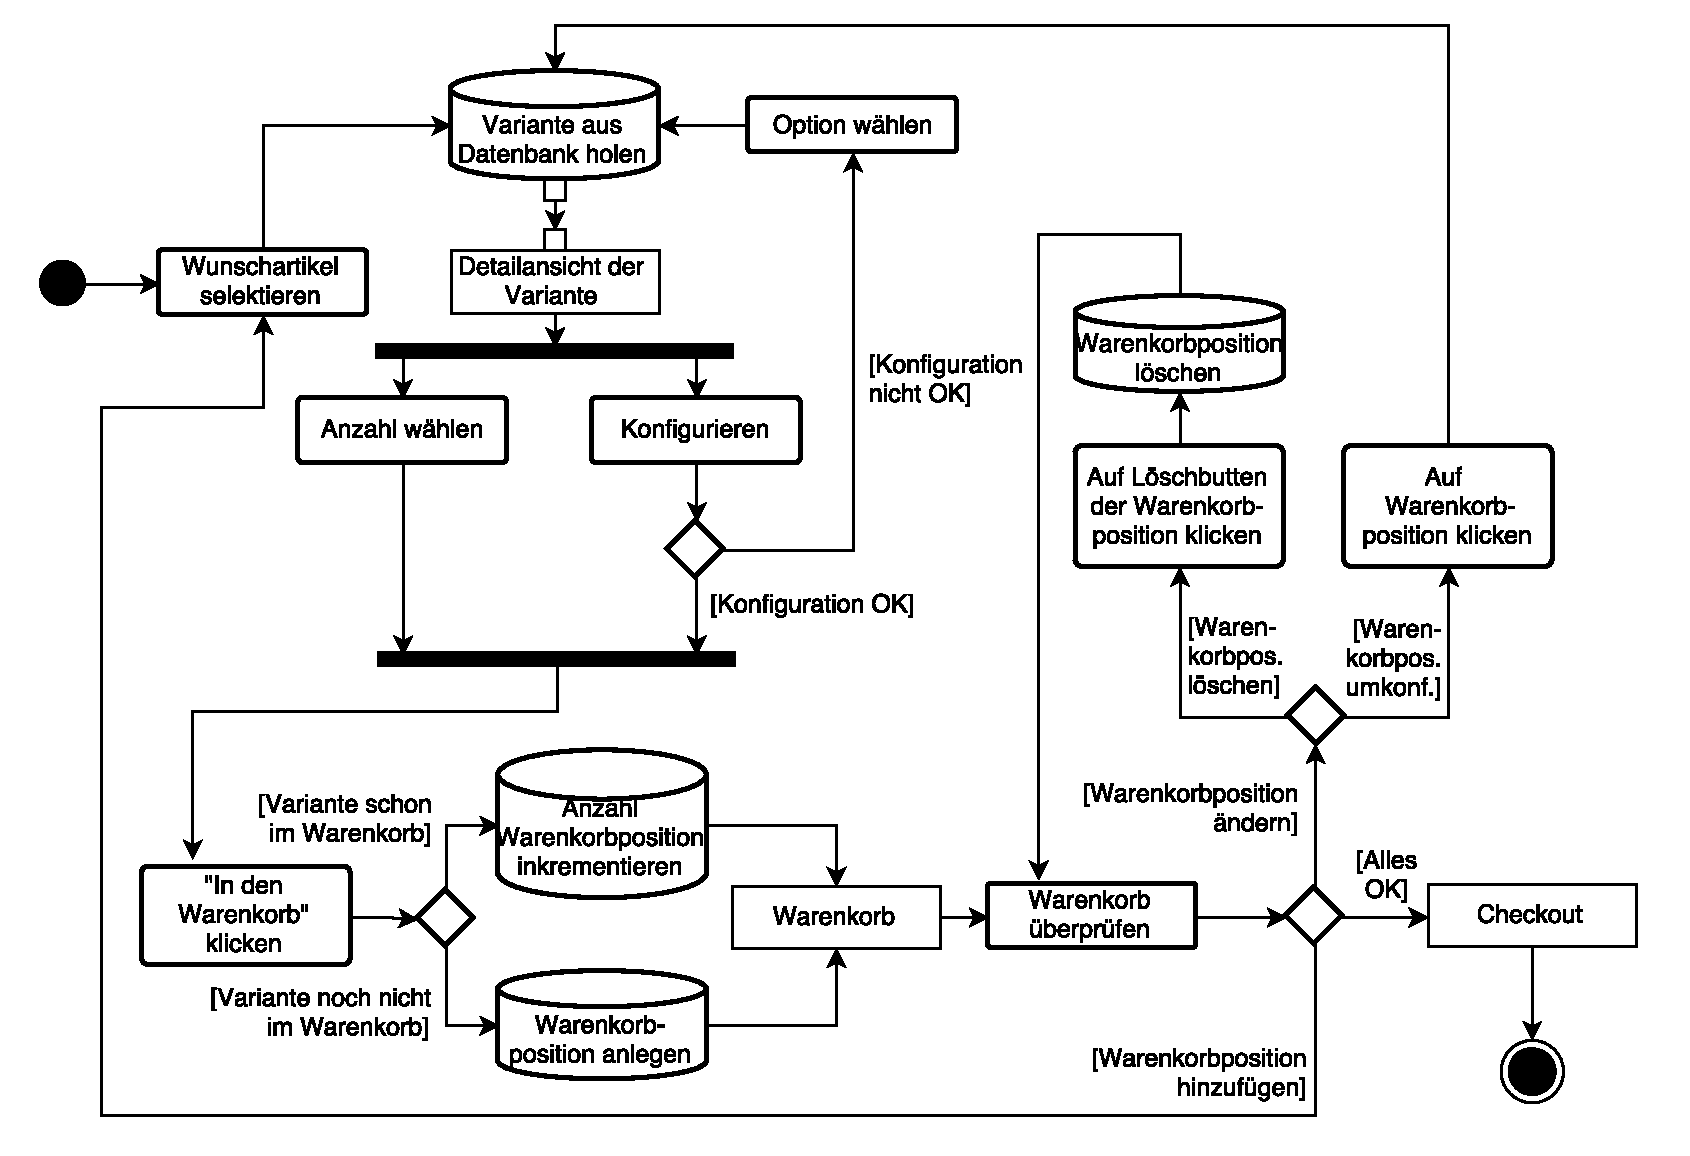
\includegraphics[width=1\linewidth]{Abbildungen/shopwareKonfigurationFlussdiagramm.pdf}
	\captionof{figure}[shopwareKonfigurationFlussdiagramm]{Aktivitätsdiagramm der Einkaufsvorgangs eines Varianten-Artikels in Shopware}
	\label{fig:shopwareKonfigurationFlussdiagramm}
\end{minipage}
\vspace{1em}

Mittels der Katalog- oder Suchfunktion wählt der Kunde einen konfigurierbaren Artikel aus - d.h., er wurde im Backend als \emph{Varianten-Artikel} gekennzeichnet. Nun wird auf der Detailseite die erste Variante des Artikels angezeigt. Dazu muss angemerkt werden, dass im Backend eingestellt werden wird, welche Variante initial geladen werden soll. Neben beschreibenden Texten und Bildern befindet sich auf der Detailseite die Konfigurationsoberfläche (siehe Abbildung \ref{app:shopwareNotebookDetail}). Zu jeder Gruppe wird ein Menü mit den entsprechenden Optionen angezeigt. Die Auswahl einer Option führt zum Reload der Seite mit der aktuellen Variante. Dieser Vorgang wiederholt sich so lange, bis der Artikel den Vorstellungen des Kunden entspricht. Außerdem wird die Anzahl eingestellt. Über den \glqq In den Warenkorb\grqq{} Button wird der Artikel in den Warenkorb gelegt. Ist diese Variante bereits im Warenkorb, wird die Anzahl der entsprechenden Warenkorbposition inkrementiert. Anderenfalls entsteht eine neue Warenkorbposition. An der jeweiligen Bezeichnung der Warenkorbposition ist ablesbar, welche Optionskombination vorliegt (siehe Abbildung \ref{app:shopwareNotebookWarenkorb}). Nun überprüft der Kunde den Warenkorb. Möchte er weitere Artikel hinzufügen, beginnt der Prozess mit der Auswahl des Wunschartikels von vorne. Ist der Kunde mit der Konfiguration einer Warenkorbposition noch nicht zufrieden, kann diese löschen oder ändern. Möchte er sie ändern, kommt er über einen Klick auf die entsprechende Position zur Detailansicht dieser Variante zurück. Nun können andere Optionen gewählt werden. Ein erneuter klick auf \glqq In den Warenkorb\grqq{} aktualisiert nicht etwa die zugehörige Warenkorbposition, sondern erzeugt einen neue. Die alte Variante verbleibt zusätzlich im Warenkorb. Ist der Nutzer mit allen Positionen im Warenkorb zufrieden, wird der Bestellvorgang über den Checkout-Prozess abgeschlossen.

Dieser Vorgang stellt den Lebenszyklus einer Variante in Shopware dar. Er beginnt mit dem Anlegen der Variante im Backend. Das ist ein Unterschied zu der Umsetzung in TCsite, welche in Kapitel \ref{subsubsection:tcsiteArchitektur}
 besprochen wurde. Hier beginnt der Lebenszyklus erst mit der Konfiguration.

\subsection{Fazit}
Shopware bietet in der Standardinstallation keine Funktionalität, die der Definition eines Konfigurationsprozesses gerecht wird. Stattdessen wird eine Variantenselektion durchgeführt. Da alle Varianten expliziert vordefiniert sind, werden dadurch die in Kapitel \ref{subssubsection:Produktklassifizierung} beschriebenen \ac{ATO}-Produkte abgebildet. Die Analyse in Kapitel \ref{subsection:Konfigurationsmodell} hat ergeben, dass das TCsite-Konfigurationsmodells auch \ac{MTO}-Produkte abbilden kann. Eine Integration des Tacton-Produktkonfigurators in Shopware würde somit dessen Angebotsspektrum in Bezug auf Produktionskonzepte erweitern.
 
Im Fazit der TCsite-Analyse (Kapitel \ref{subsubsection:tcsiteFazit}) wurde
geschlussfolgert, dass eine Konfigurationsoberfläche auch in einem externen System umsetzbar ist. Über Webcontroller kann ein Webservice implementiert werden, mit der die Konfigurationsoberfläche kommuniziert. Webcontroller werden per Plugin definiert. Für die Arbeit bedeutet dies, dass ein Plugin zu erstellen ist, welches eine Schnittstelle für externe Konfigurationsoberflächen anbietet.

In Kapitel \ref{subsubsection:shopwareErweiterbarkeit} wurde das Plugin-Konzept von Shopware vorgestellt. Die logischen Komponenten, Datenhaltung und Templates sind erweiterbar. Letzteres ermöglicht das Rendern einer Konfigurationsoberfläche in Shopware. Die Analyse des Einkaufsvorgangs von konfigurierbaren Artikeln in Kapitel \ref{subsubsection:shopwareKonfiguration} hat ergeben, wie die Varianten, die aus dem Konfigurationsprozess resultieren, ihren Lebenszyklus im Warenkorb fortsetzen. Das impliziert Änderungen über die reine Integration einer Konfigurationsoberfläche hinaus. Für die Arbeit bedeutet das, dass ein Shopware-Plugin zu erstellen ist, welches (1) eine Konfigurationsoberfläche bereitstellt und (2) die konfigurierten Artikel in den Einkaufsvorgang integriert.

Nach diesem Grobkonzept der Verantwortungsbereiche wird in der folgenden Anforderungsanalyse definiert, was die beiden Plugins im Details leisten müssen.
\pagebreak

\section{Anforderungsanalyse}
Ziel der Arbeit ist die Entwicklung eines Systems. Dieses System wird in Abbildung \ref{fig:systemcontext} in eine Beziehung mit den Elementen gebracht, welche aus der Analyse des vorherigen Kapitels hervorgehen. Der Systemkontext stellt die Umgebung dar, der die für die Entwicklung relevanten Aspekte beinhaltet. Was das System hingegen nicht beeinflusst, ist Teil der irrelevanten Umgebung.

In Kapitel \ref{fig:systemcontext} wurde erwähnt, dass die Kommunikation mit dem TCserver vom Configuration-Modul abstrahiert wird. Von außen ist also also nicht ersichtlich, dass der Konfigurationsprozess durch eine Serveranwendung realisiert wird. TCserver ist also Teil der irrelevanten Umgebung.

Zum Systemkontext gehört TCsite, da es das Configuration-Modul beherbergt. Außerdem verwaltet die Anwendung die Konfigurationsmodelle und -zustände. Weiterhin ist Shopware teil des Kontexts. Dort soll eine Konfigurationsoberfläche zur Verfügung gestellt und die resultierenden Varianten in den Einkausfsvorgang integriert werden. Der Shopkunde und -administrator sind die relevanten Stakeholder von Shopware. Sie werden mit dem Plugin interagieren.
Im Zentrum des Systemkontexts befindet sich das zu entwickelnde System selbst.

\vspace{1em}
\begin{minipage}{\linewidth}
	\centering
	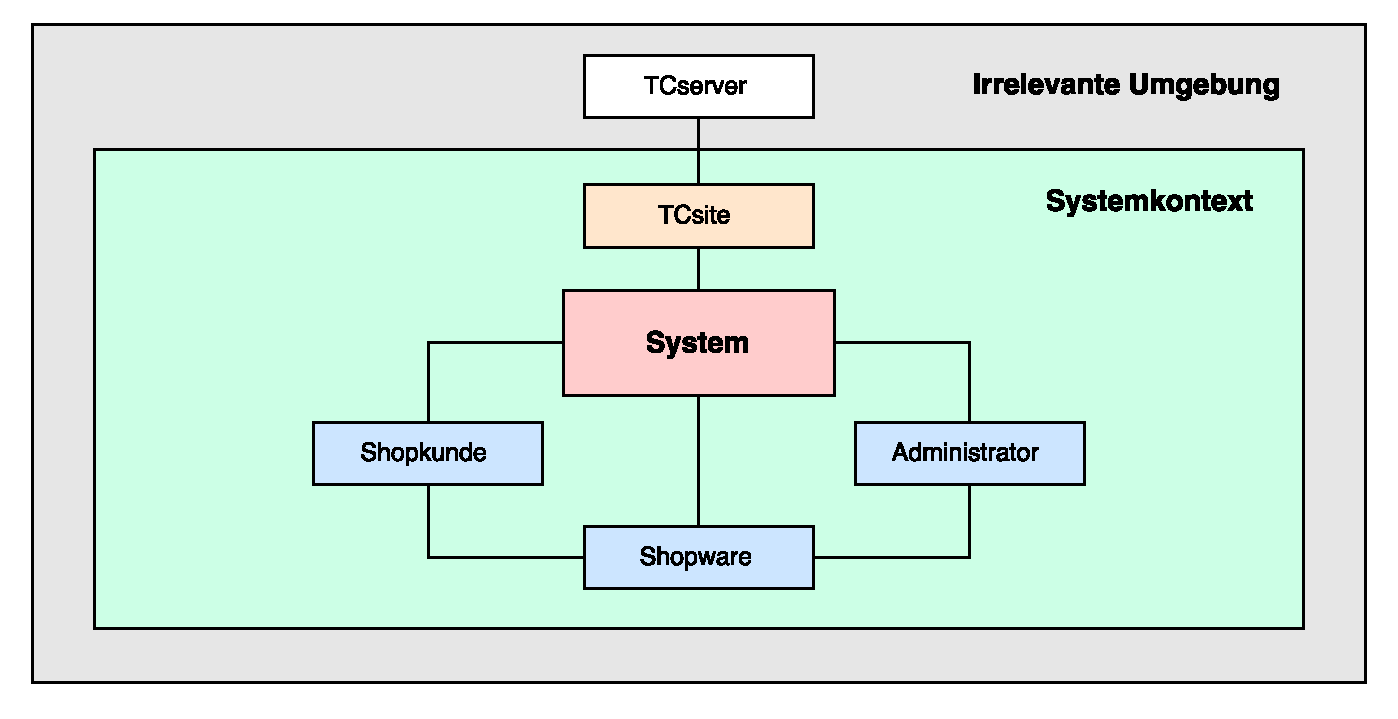
\includegraphics[width=0.8\linewidth]{Abbildungen/systemcontext.pdf}
	\captionof{figure}[systemcontext]{Systemkontext}
	\label{fig:systemcontext}
\end{minipage}
\vspace{1em}

Ausgehend von dem Fazit des vorherigen Kapitels kann das System feingranularer bestimmt werden, wie Abbildung \ref{fig:systemcontextErweitert} darstellt. Es wurde beschrieben, dass sowohl für TCsite als auch für Shopware Plugins entwickelt werden müssen. Das TCsite-Plugin stellt eine Schnittstelle als Webservice bereit, welche vom Shopware-Plugin zum rendern der Konfigurationsoberfläche genutzt wird. Darum besteht eine Verbindung zwischen beiden Plugins.
In Kapitel \ref{subsection:Webservices} wurde besprochen, dass Webservices nicht direkt von menschlichen Anwendern genutzt werden. Darum steht keiner der Stakeholder in Verbindung zum TCsite-Plugin. Hingegen werden Shopkunden im Frontend und der Administrator im Backend mit dem Shop-Plugin interagieren.

\vspace{1em}
\begin{minipage}{\linewidth}
	\centering
	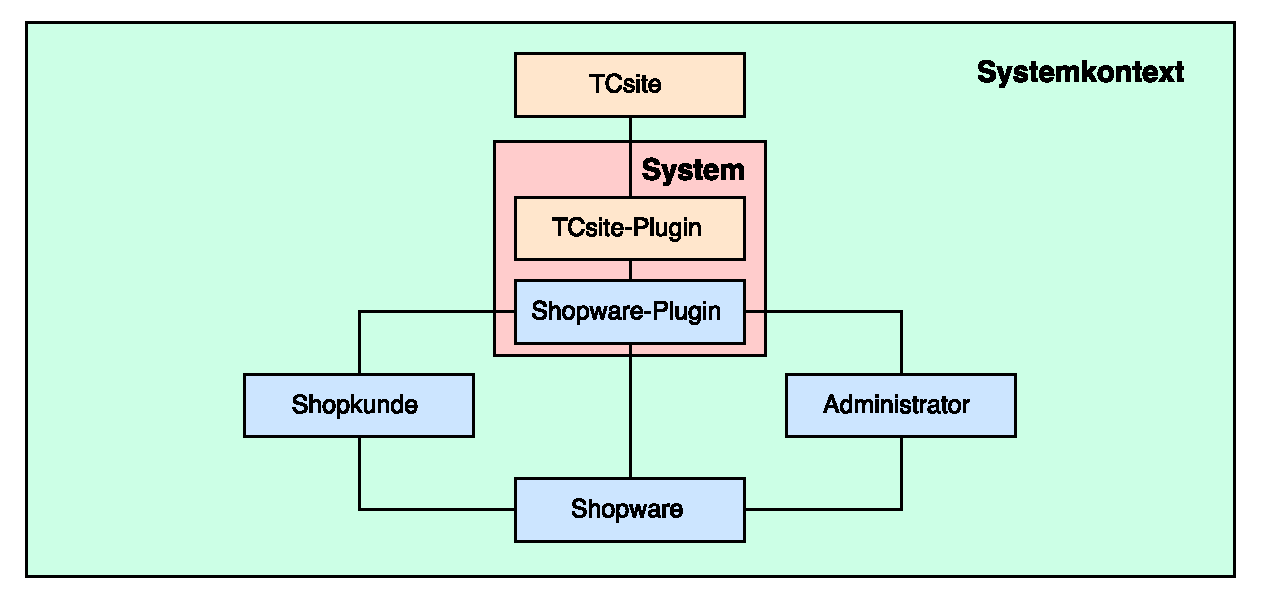
\includegraphics[width=0.8\linewidth]{Abbildungen/systemcontextErweitert.pdf}
	\captionof{figure}[systemcontextErweitert]{Systemkontext}
	\label{fig:systemcontextErweitert}
\end{minipage}
\vspace{1em}

Basierend auf den Systemkontext werden nun Anforderungen spezifiziert, die sich auf das System und die Aspekte des Systemkontexts beziehen. Es wird in funktionale und nichtfunktionale Anforderungen unterschieden.

\subsection{Funktionale Anforderungen}

Funktionale Anforderungen beschreiben das \glqq was\grqq{}, d.h. welche Funktionalitäten und Dienste das System erfüllen soll. Es werden zunächst die funktionalen Anforderungen des Shopware-Plugins erwähnt. Aus diesen ergibt sich, was das TCsite-Plugin, welches einen Webservice repräsentiert, liefern muss.

\subsubsection{Shopware-Plugin}
Die Analyse des Einkaufsvorgangs hat ergeben, dass die Konfiguration eines Artikels auf dessen Detailseite stattfindet. Daraus ergibt sich die funktionale Anforderung SW.F01:
\begin{enumerate}[SW.F01:]\bfseries
\item Das Shop-Plugin muss auf der Detailseite eine Konfigurationsoberfläche bieten.
\end{enumerate}
Die Funktionalität der Konfigurationsoberfläche kann näher beschrieben werden. Aus der Analyse des Konfigurationsprozesses in TCsite (siehe Kapitel \ref{subsubsection:tcsiteArchitektur}) ergibt sich die Anforderung SW.F02:
\begin{enumerate}[SW.F02:]\bfseries
\item Die Konfigurationsoberfläche muss einen Konfigurationsprozess äquivalent zu TCsite ermöglichen. 
\end{enumerate}
Das beinhaltet: Aktualisierung der Oberfläche nach jeder Wahl des Anwenders; Darstellung von Steps, Toplevel-Groups, optionalen Gruppen, allen Feldtypen, Hervorhebung der verhandelbar/nichtverhandelbar gewählten Optionen; Navigation durch die Execution-Struktur (Steps in vordefinierter Reihenfolge, Toplevel-Groups); Wählen von Optionen, Eingabe von Werten; Wechsel des Optionszustands zwischen verhandelbar/nichtverhandelbar; Konfliktbehebung.

Aus der Analyse des Einkaufsvorgangs in Kapitel \ref{subsubsection:shopwareKonfiguration} geht hervor, dass nach der Konfigurationen die resultierende Variante weitere Stationen durchläuft (Warenkorb, Checkout, eventuell Umkonfiguration, etc...). Daraus resultiert Anforderung SW.03, welche die Basis der folgenden Anforderungen darstellt:
\begin{enumerate}[SW.F03:]\bfseries
\item Die aus dem Konfigurationsprozess resultierende Variante muss sich in den Einkaufsvorgang integrieren.
\end{enumerate}
Damit eine Variante gekauft werden kann, benötigt sie einen Preis. Dieser wird auf der Detailseite gezeigt. Er muss entsprechend des Konfigurationsprozesses laufend aktualisiert werden. Dementsprechend lautet Anforderung SW.F04:
\begin{enumerate}[SW.F04:]\bfseries
\item Die Detailseite muss den aktuellen Preis der Variante anzeigen.
\end{enumerate}
Von der Detailseite aus kommt die Variante in den Warenkorb. Daraus ergibt sich Anforderung SW.F05:
\begin{enumerate}[SW.F05:]\bfseries
\item Die Detailseite muss das Ablegen der Variante in den Warenkorb ermöglichen.
\end{enumerate}
In Shopware wird dabei die auf der Detailseite eingestellte Anzahl berücksichtigt. Gleiches gilt implizit für Anforderung SW.F05.

In Kapitel \ref{subsubsection:tcsiteArchitektur} wurde bei der Analyse des Konfigurationsprozesses in TCsite festgestellt, dass diese erst im letzten Step abgeschlossen werden kann. Äquivalent resultiert für das Shopszenario die Anforderung SW.F06, die eine detailiertere Beschreibung der Anforderung SW.F05 darstellt:
\begin{enumerate}[SW.F06:]\bfseries
\item Die Variante muss erst im letzten Step in den Warenkorb legbar sein.
\end{enumerate}
Varianten im Warenkorb sind Warenkorbpositionen. Bei unterschiedlichen Varianten im Warenkorb muss der Kunde diese unterscheiden können. Daraus resultiert Anforderung SW.F07:
\begin{enumerate}[SW.F07:]\bfseries
\item Warenkorbpositionen müssen eine Beschreibung bieten.
\end{enumerate}
Zur Beschreibung gehört der Preis, aber zum Beispiel auch eine Zusammenfassung der gewählten Optionen.

Der in Kapitel \ref{subsubsection:shopwareKonfiguration} vorgestellte Einkaufsvorgang beinhaltet die Umkonfiguration von Warenkorbposition. Daraus resultiert Anforderung SW.F08: 
\begin{enumerate}[SW.F08:]\bfseries
\item Warenkorbpositionen muss umkonfigurierbar sein.
\end{enumerate}
Umkonfiguration wird in der Arbeit so verstanden, dass sich ändert, welche Variante eine Warenkorbposition repräsentiert. Daraus resultiert implizit, dass eine Umkonfiguration nicht zur Erstellung einer neuen, sondern zur Aktualisierung der entsprechenden Warenkorbposition führt.

Die Umkonfiguration findet auf der Detailseite statt. Dementsprechend lautet Anforderung SW.F09: 
\begin{enumerate}[SW.F09:]\bfseries
\item Die Detailseite einer Warenkorbposition muss aufrufbar sein.
\end{enumerate}
Auf der Detailseite soll die Konfiguration jedoch nicht neu beginnen, sondern dem letzten Konfigurationszustand entsprechen. Es ergibt sich Anforderung SW.F10:
\begin{enumerate}[SW.F10:]\bfseries
\item Die Detailseite muss den Konfigurationszustand einer Warenkorbposition abbilden.
\end{enumerate}
Das beinhaltet den Preis und die Konfigurationsoberfläche.

Im Einkaufsvorgang aus Kapitel \ref{subsubsection:shopwareKonfiguration} registriert der Warenkorb die Umkonfiguration erst beim erneuten Ablegen in den Warenkorb. Dementsprechend lautet Anforderung SW.F11:
\begin{enumerate}[SW.F11:]\bfseries
\item Auf der Artikeldetailseite muss die Umkonfiguration einer Warenkorbposition durch einen entsprechenden Button vom Kunden bestätigt werden.
\end{enumerate}
Durch das Umkonfigurieren kann es passieren, dass zwei Warenkorbpositionen die gleiche Variante repräsentieren. Die Varianten sollen jedoch weiterhin einzeln umkonfigurierbar sein. Daraus resultiert Anforderung SW.F13:
\begin{enumerate}[SW.F13:]\bfseries
\item Im Warenkorb muss jede Variante eine eigene Position darstellen.
\end{enumerate}
Warenkorbartikel sind auch löschbar. Daraus folgt Anforderung SW.F14:
\begin{enumerate}[SW.F14:]\bfseries
\item Im Warenkorb müssen Varianten löschbar sein.
\end{enumerate}
Die nächste Phase des Lebenszyklus ist die Bestellung. Dementsprechend lautet Anforderung SW.F15:
\begin{enumerate}[SW.F15:]\bfseries
\item In der Bestellung müssen Warenkorbpositionen übernommen werden.
\end{enumerate}
So wie die Varianten im Warenkorb beschrieben wurden, muss gleiches auch in der Bestellbestätigung stattfinden. Es resultiert Anforderung SW.F16:
\begin{enumerate}[SW.F16:]\bfseries
\item In der Bestellbestätigung für den Kunden müssen die Beschreibungen der Warenkorbpositionen übernommen werden.
\end{enumerate}
Bis jetzt wurde Unterschlagen, dass der Lebenszyklus einer Variante zwar mit der Konfiguration beginnt, auf Übersichtsseiten wie z.B. dem Artikellisting trotzdem Preise verzeichnet sind. Der Preis steht vor der Konfiguration aber noch nicht fest. Dementsprechend lautet SW.F17:
\begin{enumerate}[SW.F17:]\bfseries
\item Im Artikellisting dürfen konfigurierbare Artikel keinen Preis auszeichnen.
\end{enumerate}
Ein eShop bietet nicht nur konfigurierbare Artikel an. Dementsprechend muss das Plugin einen Mechanismus anbieten, über den im Backend eingestellt wird, welche Artikel per das Plugin konfigurierbar sind und welche nicht. Daraus ergibt sich Anforderung SW.F18:
\begin{enumerate}[SW.F18:]\bfseries
\item Das Shop-Plugin muss dem Administrator im Backend eine Angabe darüber ermöglichen, ob ein Artikel per Plugin konfigurierbar ist.
\end{enumerate}
Wenn ein Artikel per Plugin konfigurierbar ist, stellt sich die Frage, welchem Konfigurationsmodell die Konfiguration es entsprechen soll. In TCsite sind Konfigurationsmodelle Produkten zugeordnet. Daraus ergibt sich Anforderung SW.F19:
\begin{enumerate}[SW.F19:]\bfseries
\item Das Shop-Plugin muss dem Administrator im Backend eine Angabe darüber ermöglichen, welchem TCsite-Produkt ein Artikel entspricht.
\end{enumerate}
So wird die Zuordnung händisch vom Shopware-Administrator hergestellt. Er muss also auch Kenntnis von den in TCsite verfügbaren Produkten haben.

Abschließend muss das Plugin noch die Adresse des Webservices kennen, welches durch das TCsite-Plugins implementiert wird. Es folgt Anforderung SW.F20:
\begin{enumerate}[SW.F20:]\bfseries
\item Das Shop-Plugin muss dem Administrator im Backend eine Angabe darüber ermöglichen, unter welcher URI das TCsite-Plugin erreichbar ist.
\end{enumerate}

\subsubsection{TCsite-Plugin}
Aus den Anforderungen des Shopware-Plugins ergeben sich die Anforderungen des TCsite-Plugins.

SW.F02 fordert Daten, auf deren Grundlage die Konfigurationsoberfläche gerendert werden kann. Dementsprechend lautet Anforderung TC.F01:
\begin{enumerate}[TC.F01:]\bfseries
\item Das TCsite-Plugin muss die Informationen zum Aufbau der Konfigurationsoberfläche bereitstellen.
\end{enumerate}
Aus SW.F10 ergibt sich, dass das Shopware-Plugin auch nach Abschluss der Konfiguration im Falle einer Umkonfiguration die Konfigurationsoberfläche erneut rendern muss. Ob und wann eine Umkonfiguration stattfindet, ist nicht klar. Daraus ergibt sich Anforderung TC.F02:
\begin{enumerate}[TC.F02:]\bfseries
\item Die Informationen zum Aufbau der Konfigurationsoberfläche müssen persistiert werden.
\end{enumerate}
Weiterhin muss das Shopware-Plugin wissen, wie es diese persistenten Informationen zu einem späteren Zeitpunkt wieder abrufen kann. Daraus ergibt sich Anforderung TC.03:
\begin{enumerate}[TC.F03:]\bfseries
\item Das TCsite-Plugin muss Informationen zum späteren Aufbau der Konfigurationsoberfläche bereitstellen.
\end{enumerate}
Im Fazit aus Kapitel \ref{subsubsection:tcsiteFazit} wurde festgelegt, dass über die Oberfläche die gewählten Optionen des Shopkunden erfasst werden, der technische Konfigurationsprozess aber durch das TCsite-Plugin realisiert wird. Daraus ergibt sich Anforderung TC.04:
\begin{enumerate}[TC.F04:]\bfseries
\item Das TCsite-Plugin führt den technischen Konfigurationsprozess durch.
\end{enumerate}
Neben den Daten für die Oberfläche fordert SW.F04 Preisinformation. Dementsprechend lautet Anforderung TC.F04:
\begin{enumerate}[TC.F04:]\bfseries
\item Das TCsite-Plugin muss Informationen über den Preis einer Variante bereitstellen.
\end{enumerate}
Abschließend fordert SW.F07 nach einer Beschreibung von Warenkorbpositionen. Es resultiert Anforderung TC.F05:
\begin{enumerate}[TC.F05:]\bfseries
\item Das TCsite-Plugin muss die Beschreibung einer Variante bereitstellen.
\end{enumerate}

\subsection{Nichtfunktionale Anforderungen}
Nichtfunktionale Anforderungen beschreiben das \glqq wie\grqq{}, d.h. welche Eigenschaften das System besitzen soll.

\subsubsection{Shopware-Plugin}
Wie bereits erwähnt, werden die Funktionalitäten im Rahmen eines Plugins implementiert. Die Anforderung SW.NF01 lautet dementsprechend:
\begin{enumerate}[SW.NF01:]\bfseries
\item Integration des Tacton-Produktkonfigurators muss über ein Shop-Plugin umgesetzt werden.
\end{enumerate}
Weiterhin kann aufgrund der technischen Analyse eine Aussage darüber getroffen werden, mit welchen Programmiersprachen das Shop-Plugin zu entwickeln ist. In der View kommt Smarty-Syntax zum Einsatz, wobei Javascript und CSS eingebunden werden kann. Die logischen Erweiterungen werden in PHP verfasst. Anforderung SW.NF02 lautet demzufolge:
\begin{enumerate}[SW.NF02:]\bfseries
\item Das Shop-Plugin muss unter der Verwendung von PHP, Smarty-Syntax, Javascript, und CSS erstellt werden.
\end{enumerate}

\subsubsection{TCsite-Plugin}
Die nichtfunktionalen Anforderungen des TCsite-Plugins fallen äquivalent aus. TC.NF01 lautet:
\begin{enumerate}[TC.NF01:]\bfseries
\item Die Konfigurationsschnittstelle muss über ein TCsite-Plugin umgesetzt werden.
\end{enumerate}
In Kapitel \ref{subsection:TCsite} wurde erwähnt, dass die Architektur in Java implementiert ist. Daraus resultiert für die Anforderung TC.NF02:
\begin{enumerate}[TC.NF02:]\bfseries
\item Das TCsite-Plugin muss unter der Verwendung von Java erstellt werden.
\end{enumerate}
Aus dem Erweiterungskonzept von TCsite (siehe Kapitel \ref{subsubsection:Erweiterbarkeit})
 kann schon jetzt das zu verwendende Webservice-Paradigma abgeleitet werden. Im Fazit des vorangegenen Kapitels wurde festgelegt, dass Web-Controller genutzt werden. Entsprechend des Kurfazits in Kapitel \ref{subsection:Webservices} steht damit das Werkzeug zur Implementierung eines REST-Websservices zur Verfügung. Es resultiert die Anforderung:
\begin{enumerate}[TC.NF04:]\bfseries
\item Die Konfigurationsschnittstelle wird als Webservice entsprechend des REST-Architekturstils implementiert.
\end{enumerate}

\pagebreak

\section{Konzeption}
\textbf{Vorgehensweise}\\
Aus der Anforderungsanalyse ist hervorgegangen, dass zwei Plugins konzipiert werden müssen. Es wird erst das Shopware-Plugin und danach das TCsite-Plugin behandelt. Grund dafür ist, dass das TCsite-Plugin einen Webservice darstellt, den das Shopware-Plugin als Client nutzt. Indem der Client zuerst konzipiert wird, ergeben sich daraus die Ressourcen und Prozesse, die vom Service bereitgestellt werden müssen.

\subsection{Shopware-Plugin}
Vor der Konzeption des Shopware-Plugins wird betrachtet, wie sich Artikel, Varianten, Warenkorbpositionen etc. zueinander im Datenbankschema von Shopware verhalten. Daraus wird abgeleitet, wie die Ergebnisse einer Konfiguration -- die Varianten -- in den Einkaufsvorgang integriert werden. Dabei wird beantwortet, neue Klassen bzw. Tabellen erzeugt oder bestehende Strukturen verwendet werden können.

\vspace{1em}
\begin{minipage}{\linewidth}
	\centering
	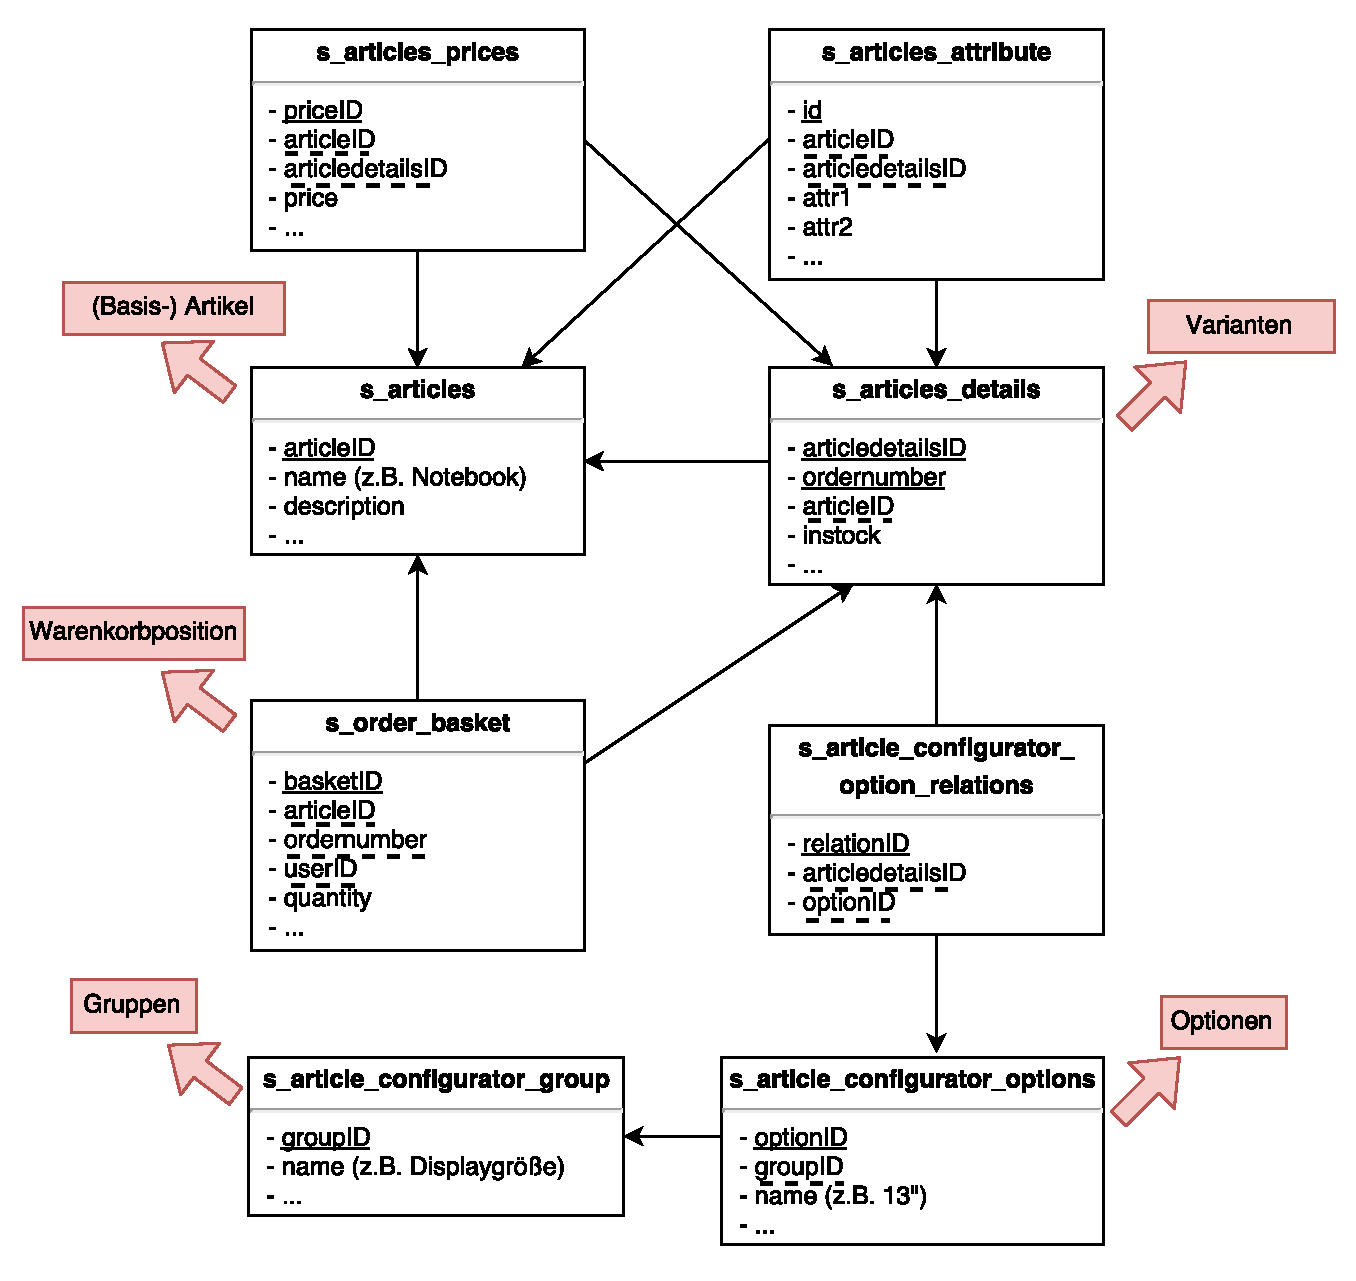
\includegraphics[width=0.7\linewidth]{Abbildungen/shopwareArtikelRelationenModell.pdf}
	\captionof{figure}[shopwareArtikelRelationenModell]{Ausschnitt des Relationenmodells in Shopware}
	\label{fig:shopwareArtikelRelationenModell}
\end{minipage}
\vspace{1em}

Abbildung \ref{fig:shopwareArtikelRelationenModell} zeigt den für die Konzeption wichtigen Ausschnitt des Shopware-Datenbankschemas als Relationenmodell. Eine vollständige Übersicht ist Quelle \citet{shopwareDatabaseScheme} zu entnehmen. Auf der Abbildung sind die im Analysekapitel \ref{subsection:Shopsystem} verwendeten Begriffe rot zugeordnet. Dem Relationenmodell ist zu entnehmen, dass Artikel (\emph{s\_articles}) und deren Varianten (\emph{s\_articles\_details}) in unterschiedlichen Tabellen gespeichert werden. Artikel und Varianten stehen in einer 1-zu-n Beziehung. Die Varianten kennen den jeweiligen Basisartikel, aber nicht umgekehrt. Es ist anzumerken, dass auch zu einem variantenlosen Artikel zumindest eine Zeile in \emph{s\_articles\_details} angelegt wird. Der Artikel und die Variante stehen dann in einer 1-zu-1 Beziehung (kann im Relationenschema nicht ausgedrückt werden). Daraus lässt sich ableiten, dass in \emph{s\_articles} Informationen stehen, die für alle Varianten gelten (z.B. die allgemeine Produktbeschreibung \emph{description}) während \emph{s\_articles\_details} detailliertere Informationen enthält (z.B. der jeweilige Lagerbestand \emph{instock}). Es ist hervorzuheben, dass \emph{s\_articles\_details} zwei Primärschlüssel besitzt, die jeweils eindeutig sein müssen -- \emph{articledetailsID} und \emph{ordernumber}. Die \emph{articledetailsID} wird vom System vergeben, während die \emph{ordernumber} vom Administrator bestimmt werden kann. Somit ist die \emph{ordernumber} ein menschenlesbarer Identifikator, der vom Vertrieb zugeordnet kann.

Die Verbindung zwischen einer Variante und den Optionen (\emph{s\_article\_configurator\_options }), aus denen sie generiert wurde, wird über die Tabelle \emph{s\_article\_configurator\_option\_relations} hergestellt. Weder sind Optionen inhärenter Bestandteil einer Variante, noch besitzt diese unmittelbare Fremdschlüsselverweise auf Optionen. Damit ist eine Variante nicht existentiell auf Optionen angewiesen. Daraus wird geschlussfolgert, dass im Einkaufsprozess Varianten dynamisch, d.h. bei Bedarf, generiert werden können.

Im Gegensatz dazu hat eine Warenkorbposition (\emph{s\_order\_basket}) einen obligatorischen Fremdschlüsselverweis auf eine Variante -- und ist damit von deren Existenz abhängig. Ein Warenkorbposition kann zeitlich nicht vor der zugehörigen Variante angelegt werden. Es wird geschlussfolgert, dass eine Variante noch nicht zum Beginn des Einkaufsvorgangs, aber spätestens beim Ablegen in den Warenkorb erstellt werden muss. Damit steht der zeitliche Spielraum für die dynamische Variantengenerierung fest.

\subsubsection{Einkaufsvorgang}
Abbildung \ref{fig:konzeptionEinkausvorgang1} stellt den neuen Einkaufsvorgang dar. Er entsteht aus dem Einkaufsvorgang in Abbildung \ref{fig:shopwareKonfigurationFlussdiagramm}, wenn folgende Sachverhalte berücksichtigt werden:
\begin{enumerate}
\item Es wird mit dem TCsite-Plugin kommuniziert (dargestellt als Wolken).
\item Varianten werden dynamisch angelegt.
\item Werden Warenkorbpositionen umkonfiguriert, entsteht keine neue Warenkorbposition, sondern die Warenkorbposition wird aktualisiert.
\end{enumerate}

\vspace{1em}
\begin{minipage}{\linewidth}
	\centering
	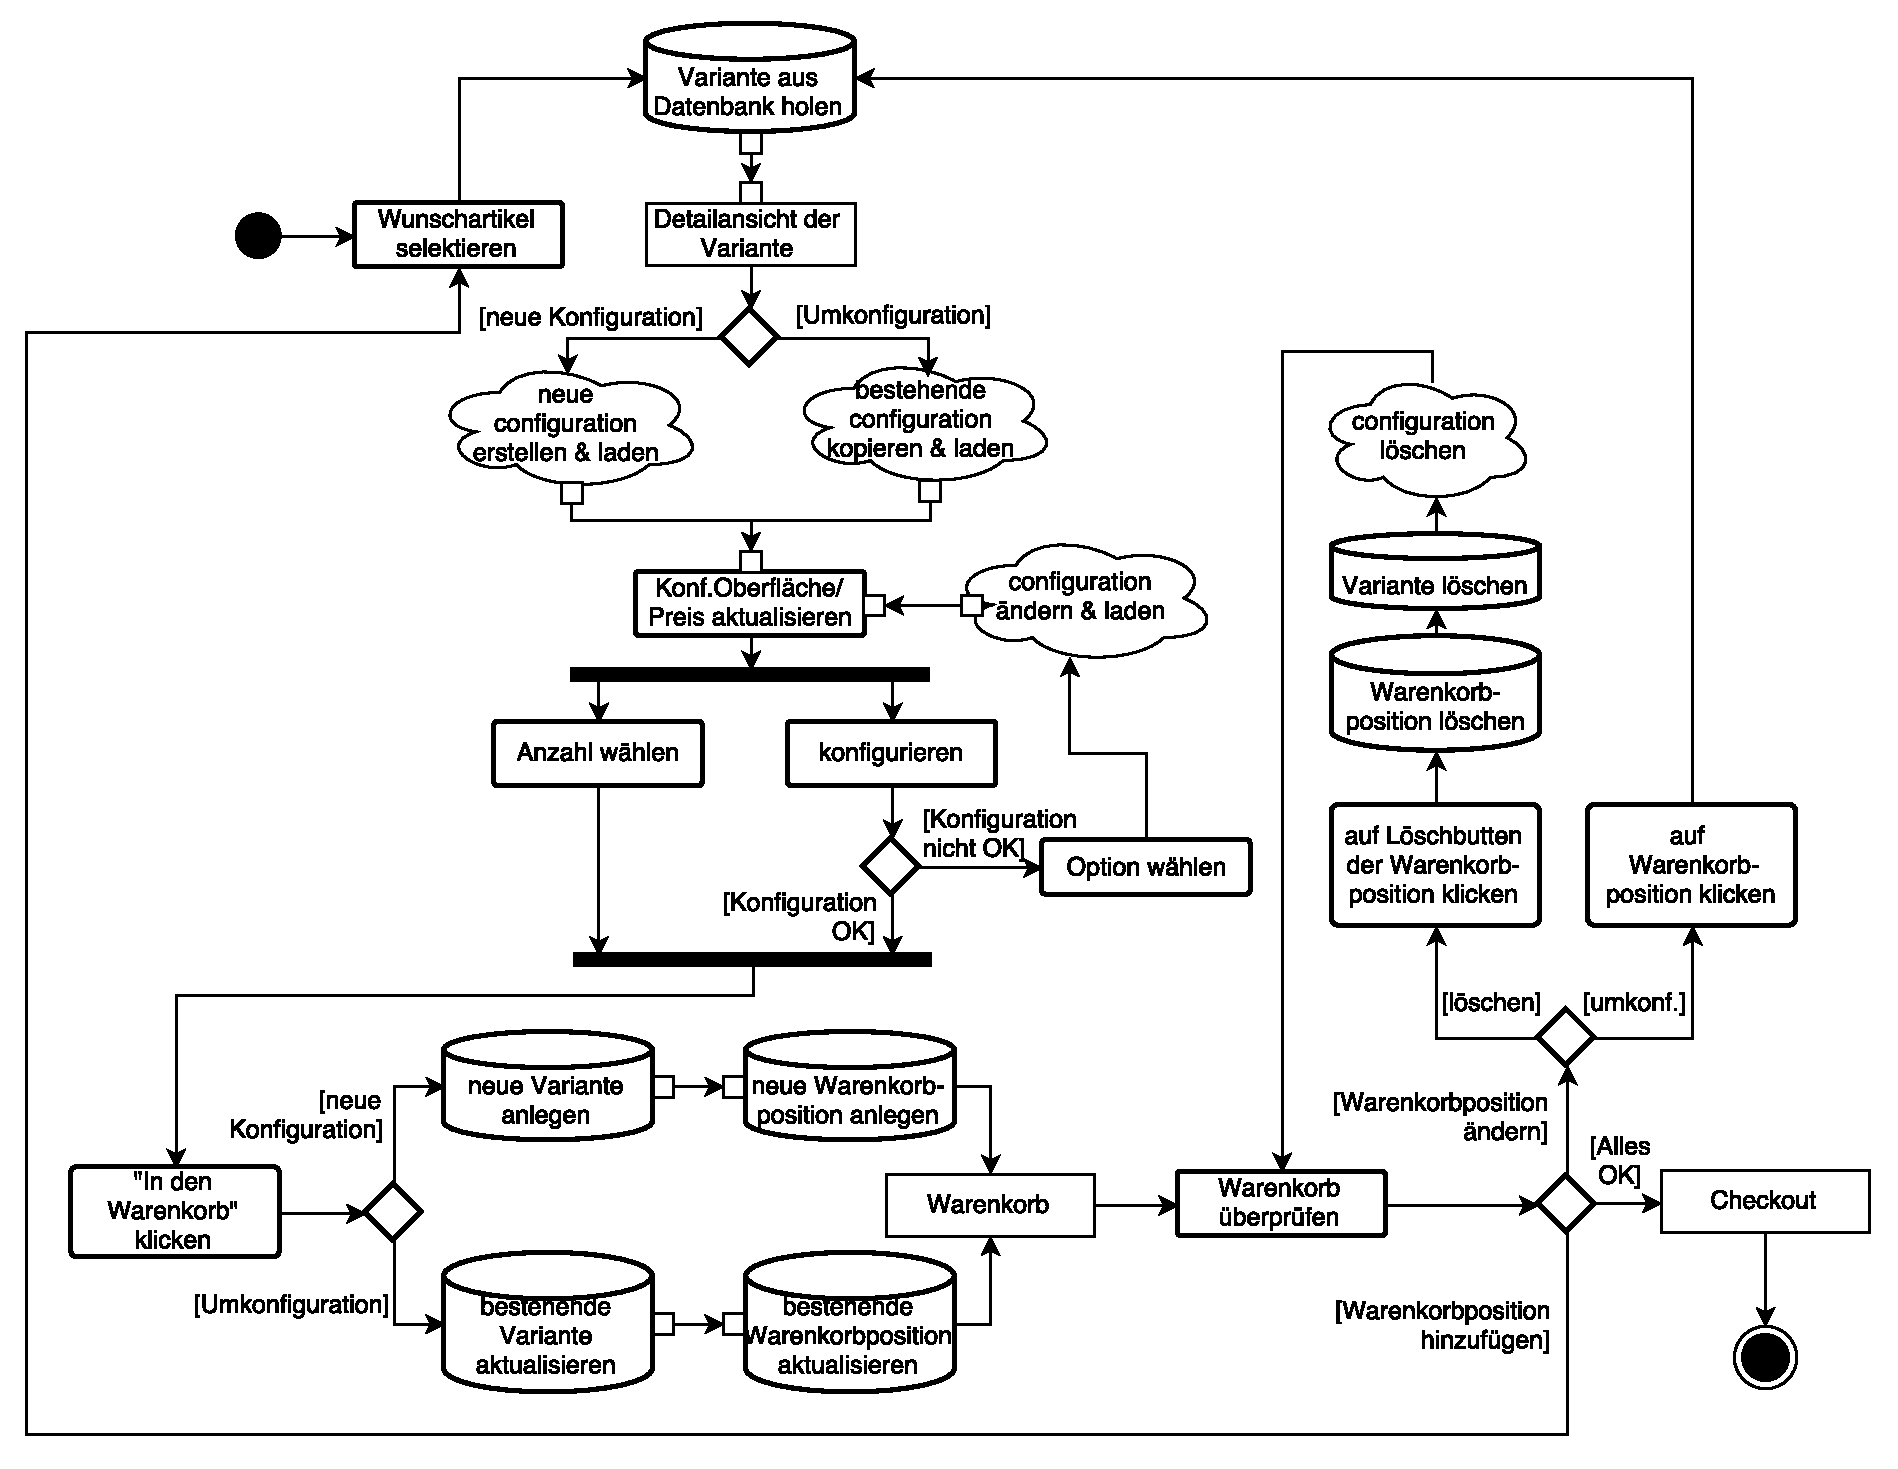
\includegraphics[width=1\linewidth]{Abbildungen/konzeptionEinkausvorgang1.pdf}
	\captionof{figure}[konzeptionEinkausvorgang1]{Aktivitätsdiagramm des Einkaufsvorgangs von Artikeln, die per Plugin konfiguriert werden}
	\label{fig:konzeptionEinkausvorgang1}
\end{minipage}
\vspace{1em}

Das Aktivitätsdiagramm (Abbildung \ref{fig:konzeptionEinkausvorgang1}) bildet den \glqq roten Faden\grqq{} für die folgende Konzeption. Während der chronologischen Erläuterung des Einkaufsvorgangs werden die Daten und Prozesse erläutert, die vom Service bereit gestellt werden müssen. Gleichzeitig wird besprochen, welche Modifikationen der Shopware-Funktionalität vorgenommen werden müssen und welche der Erweiterungskonzepte aus Kapitel \ref{subsubsection:shopwareErweiterbarkeit} dafür jeweils in Frage kommen.

\textbf{Artikellisting}\\
Der Einkaufsvorgang beginnt mit dem Auswählen des gewünschten Artikels. Das kann über verschiedene Wege passieren, zum Beispiel über das Artikellisting. Abbildung \ref{app:shopwareArtikelListing} zeigt, dass dabei standardmäßig Preise angezeigt werden. Gemäß Anforderung \emph{SW.F17} dürfen konfigurierbare Artikel aber keinen Preis ausweisen. Es muss also ein Hinweis darüber hinterlegt werden, welche Artikel per Plugin konfigurierbar sind. Das entspricht Anforderung \emph{SW.F17}, gemäß derer im Backend markierbar sein muss, welche Artikel konfigurierbar sind. Gleichzeitig muss gemäß Anforderung \emph{SW.F18} hinterlegt werden, welchem Produkt in TCsite ein Shopware-Artikel entsprechen soll. Im Folgenden wird diese Zuordnung als \emph{korrespondierendes TCsite-Produkt} bezeichnet. Es wird festgelegt: besitzt ein Artikel diese Zuordnung, ist es per Plugin konfigurierbar.

Zum Hinterlegen der Zuordnung wird eine Datenbank-Erweiterung genutzt. Konkret wird das in Kapitel \ref{subsubsection:shopwareErweiterbarkeit} angesprochene System der Attributtabellen verwendet, welchen Plugins leicht Spalten hinzufügen können. Abbildung \ref{fig:shopwareArtikelRelationenModell} zeigt \emph{s\_articles\_attributes}, die Attributtabelle von Artikeln und ihren Varianten. Shopware legt zu jeder Variante in \emph{s\_articles\_details} automatisch eine zugehörige Zeile in der Attributtabelle an. Es wird die Entwurfsentscheidung getroffen, der Tabelle eine Spalte \emph{correspondingTcsiteProduct} hinzuzufügen. Um diese Spalte befüllen zu können, kann ein entsprechendes Textfeld per \emph{Ext JS}-Erweiterung dem Artikelmenü (dargestellt in Abbildung \ref{app:shopwareBackendArtikel}) hinzugefügt werden. In Kapitel \ref{subsubsection:shopwareErweiterbarkeit} wurde außerdem erwähnt, dass in Smarty-Templates logische Einheiten existieren, die als Blöcke bezeichnet werden. Der Block namens \emph{frontend\_listing\_box\_article\_price\_default} beinhaltet den Preis eines Artikels im Artikellisting.  Über eine Template-Erweiterung muss dieser Block ersetzt werden. Er soll künftig überprüfen, ob ein Eintrag über eine korrespondierendes TCsite-Produkt vorliegt und die Ausgabe entsprechend anpassen (z.B. statt Anzeige des Preises \glqq Preis entsprechend Konfigruation\grqq{}. Somit werden die Anforderungen \emph{SW.F17}, \emph{SW.F18} und \emph{SW.F19} erfüllt.

\textbf{Detailseite}\\
Der Anwender befindet sich nur auf der Detailseite eines konfigurierbaren Artikels. Dieser wurde im Backend nie als \emph{Varianten-Artikel} markiert. Darum wird nicht der Standard-Konfigurationsmechanismus von Shopware getriggert und demzufolge auch kein Konfigurationsmenü wie in Abbildung \ref{app:shopwareNotebookDetail} angezeigt.

Stattdessen startet nun der Konfigurationsprozess über das Shopware-Plugin. Dazu müssen Daten vom TCsite-Plugin geladen werden. Diese Daten werden im Rest der Konzeption des Shopware-Plugins unter dem Begriff \textbf{configuration} zusammengefasst. Aus Shopware-Sicht ist das ein Aggregat, welches alle Informationen zum Rendern der Konfigurationsoberfläche und zur Integration der entstehenden Variante in den Einkaufsvorgang enthält. Ob und wie dieses Aggregat als einzelne Ressourcen modelliert wird, ist Verantwortungsbereich der späteren Webservice-Konzeption. Fest steht jetzt bereits, dass die Daten der \emph{configuration} als JSON präsentiert werden. TCsite hat für Webcontroller bereits Komponenten zum serialisieren und deserialisieren von JSON-Objekten eingebaut \citep{tactonTCsiteDevelopmentManual}.

\vspace{1em}
\begin{minipage}{\linewidth}
	\centering
	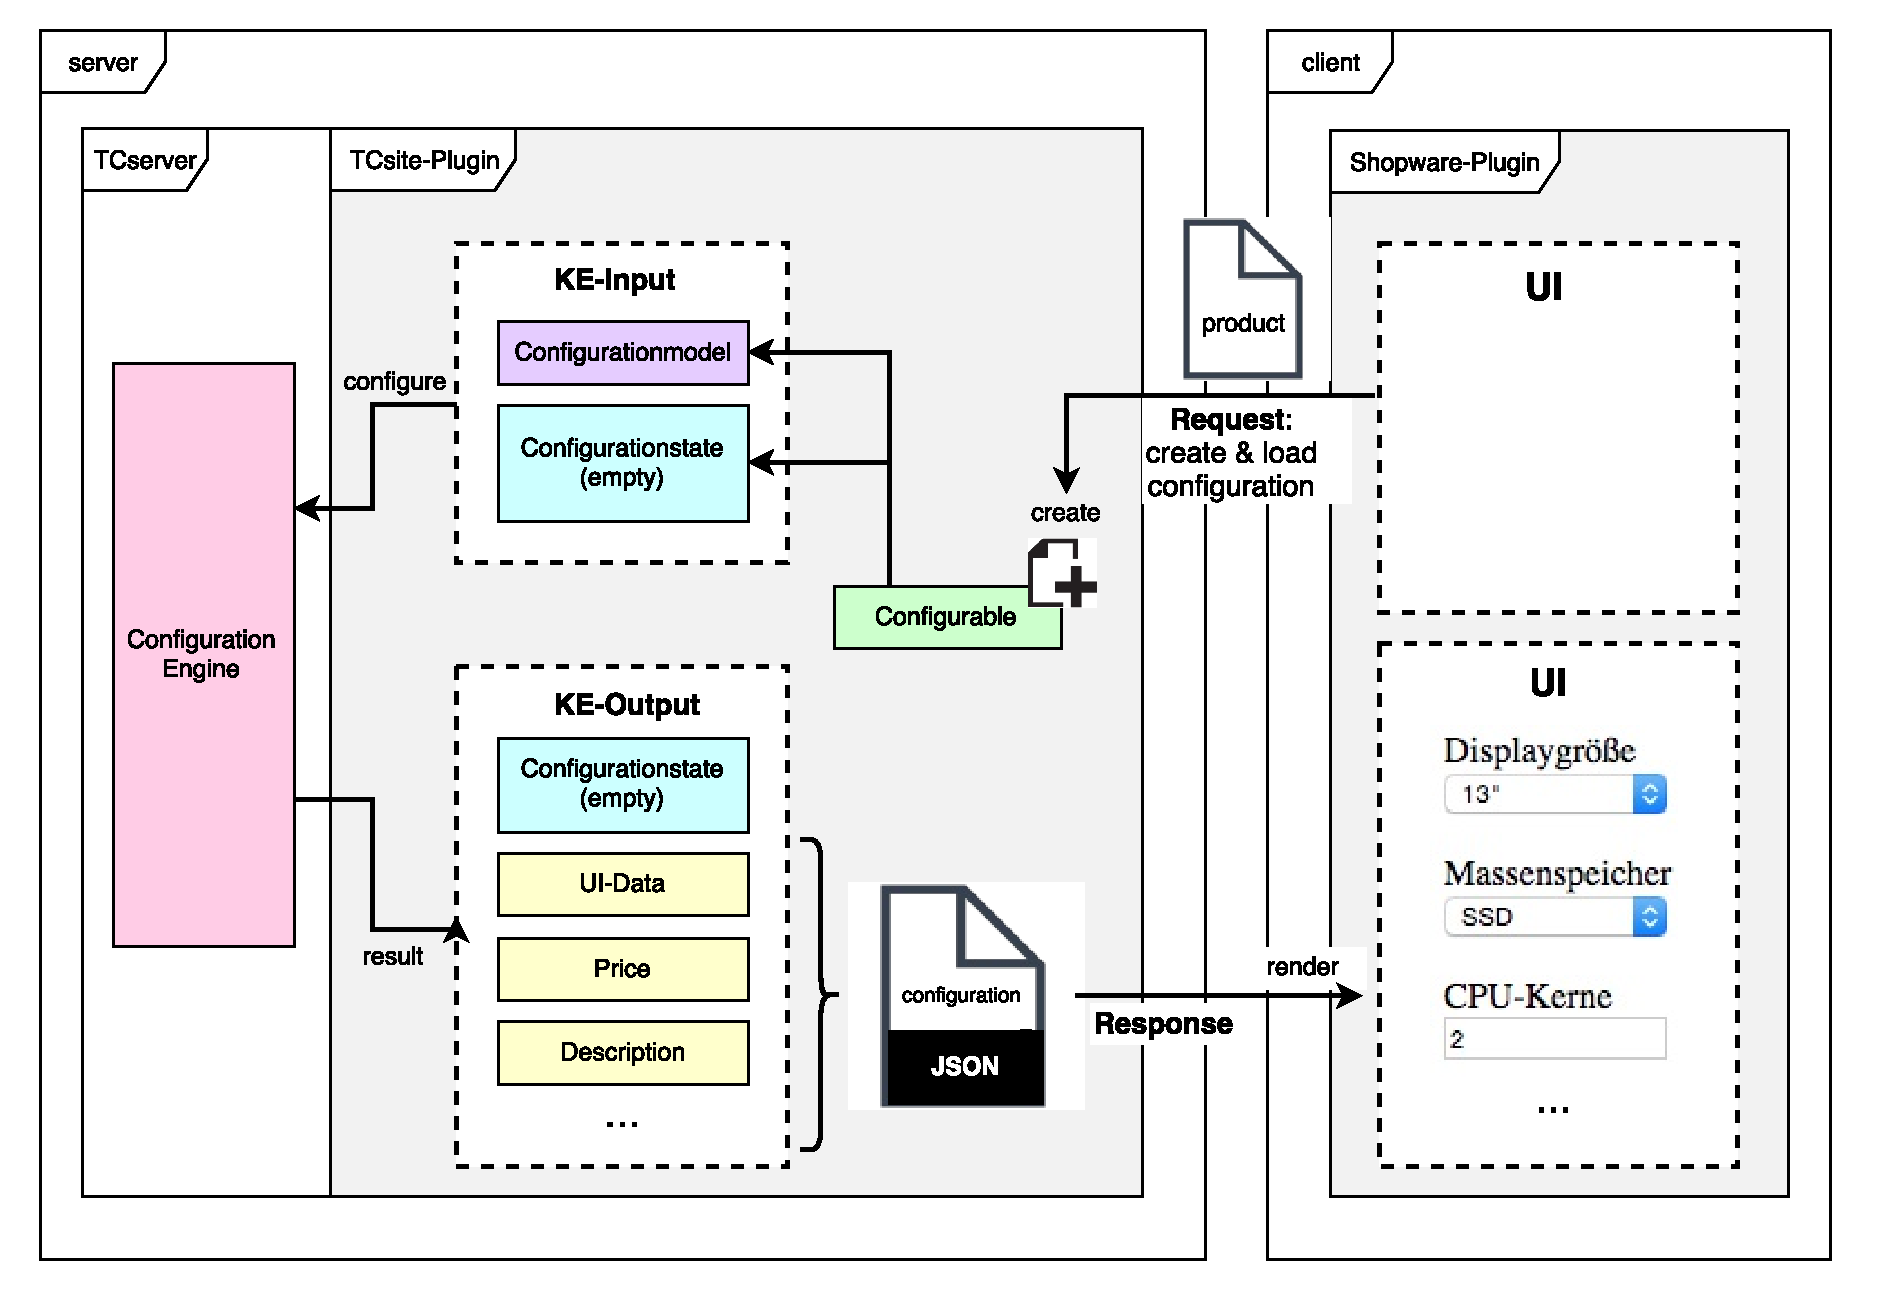
\includegraphics[width=1\linewidth]{Abbildungen/konzeptCreate.pdf}
	\captionof{figure}[konzeptCreate]{Erstellen \& Laden einer neuen \emph{configuration}-Ressource}
	\label{fig:konzeptCreate}
\end{minipage}
\vspace{1em}

Abbildung \ref{fig:konzeptCreate} zeigt, wie das Erstellen \& Laden der \emph{configuration} abläuft. Sie stellt gleichzeitig eine Detailansicht der Prozesse dar, die in der Phase \emph{initiate configuration} der Abbildung  \ref{fig:tcsiteTCserverCommunication} stattfinden. Das Shopware-Plugin teilt dem TCsite-Plugin mit, für welches Produkt (z.B. ein Notebook) eine Konfiguration starten soll. Das TCsite-Plugin erstellt und speichert ein \emph{configurable}-Objekt, welches das entsprechende Konfigurationsmodell (z.B. ein Notebook-Konfigurationsmodell) und einen Konfigurationszustand enthält. Der Konfigurationszustand ist noch leer, da zu diesem Zeitpunkt noch keine Optionen gewählt wurden. Daraus wird ein \emph{KE-Input} definiert, der mit einem \emph{KE-Output} beantwortet wird. Aus diesem werden die relevanten Informationen als JSON verpackt und dem Shopware-Plugin geschickt.

Das \emph{configurable} verwaltet ab jetzt den Konfigurationszustands dieser Konfiguration. In der Antwort des TC-Site-Plugins muss also eine Information darüber enthalten sein, wie das Shop-Plugin genau die \emph{configuration}-Ressource wiederfinden kann, die mit dem \emph{configurable} im Zusammenhang steht. Diese Information wird von nun an als \emph{configurationID} bezeichnet. Dementsprechend wird die Datenbanktabelle \emph{s\_articles\_details} um eine weitere Spalte \emph{configurationID} ergänzt. Damit sind alle notwendigen Datenbank-Erweiterungen abgeschlossen. Zusammenfassend wird die Tabelle \emph{s\_articles\_details} um zwei neue Spalten ergänzt -- \emph{correspondingTcsiteProduct} und \emph{configurationID}. Die \emph{configurationID} wird jedoch erst in die Datenbank eingetragen, wenn die entsprechende Variante nach Abschluss der Konfiguration in den Warenkorb gelegt wird.

Die Beschreibung des Aktivitätsdiagramms (Abbildung \ref{fig:konzeptionEinkausvorgang1}) wird fortgeführt. Oben wurde der Punkt \glqq neue configuration erstellen \& laden\grqq behandelt. Die Erläuterung von \glqq bestehende configuration kopieren \& laden\grqq folgt zu einem späteren Zeitpunkt. Es folgt das initiale Rendern der Konfigurationsoberfläche und die Aktualisierung der Preisanzeige mittels der Daten aus der \emph{configuration}-Ressource. Hierfür werden Template-Erweiterungen genutzt. Der Smarty-Block \emph{frontend\_detail\_index\_detail} zeichnet den Bereich der Detailseite aus, der das Artikelbild enthält (siehe Abbildung \ref{app:shopwareNotebookDetail}). Unterhalb wird die Konfigurationsoberfläche angehangen. Die original Preisanzeige wird per DOM-Manipulation aktualisiert. Sowohl für die DOM-Manipulation als auch für das Rendern der Konfigurationsoberfläche wird clientseitige Logik, d.h. Javascript, benötigt. Für das Einbinden eigener Javascript-Dateien steht der Smarty-Block \emph{frontend\_index\_header\_javascript} zur Verfügung.

\textbf{Konfigurationsprozess}\\
Es folgt der Konfigurationsprozess. Der Anwender wählt über die Konfigurationsoberfläche Optionen, tätigt Eingaben und wechselt Steps. Abbildung \ref{fig:konzeptChange} stellt die Kommunikation zwischen dem Shopware-Plugin und dem TCsite-Plugin nach jeder Nutzerinteraktion dar.

Das Shopware-Plugin übermittelt die gewählte Option an das TCsite-Plugin. Außerdem muss die \emph{configurationID} mit übertragen werden, die das Shopware-Plugin beim initialen Anfordern der \emph{configuration} erhalten hat. So kann das TCsite-Plugin zuordnen, auf welche \emph{configuration}-Ressource sich die Option bezieht. Das entsprechende \emph{confgiruable} wird geladen. In Verbindung mit der gewählten Option des Anwenders wird ein \emph{KE-Input} definiert. Der KE-Output enthält den neuen Konfigurationszustand. Das \emph{configurable} entsprechend aktualisiert und gespeichert. Die Daten für die \emph{configuration}-Ressource spiegeln den neuen Konfigurationszustand wieder. Sie werden an das Shopware-Plugin zurückgesendet. Dort werden wiederum Konfigurationsoberfläche und Preisanzeige aktualisiert. Dieser Prozess wiederholt sich solange, bis der Anwender im letzten Step angekommen und mit allen Optionen zufrieden ist.

\vspace{1em}
\begin{minipage}{\linewidth}
	\centering
	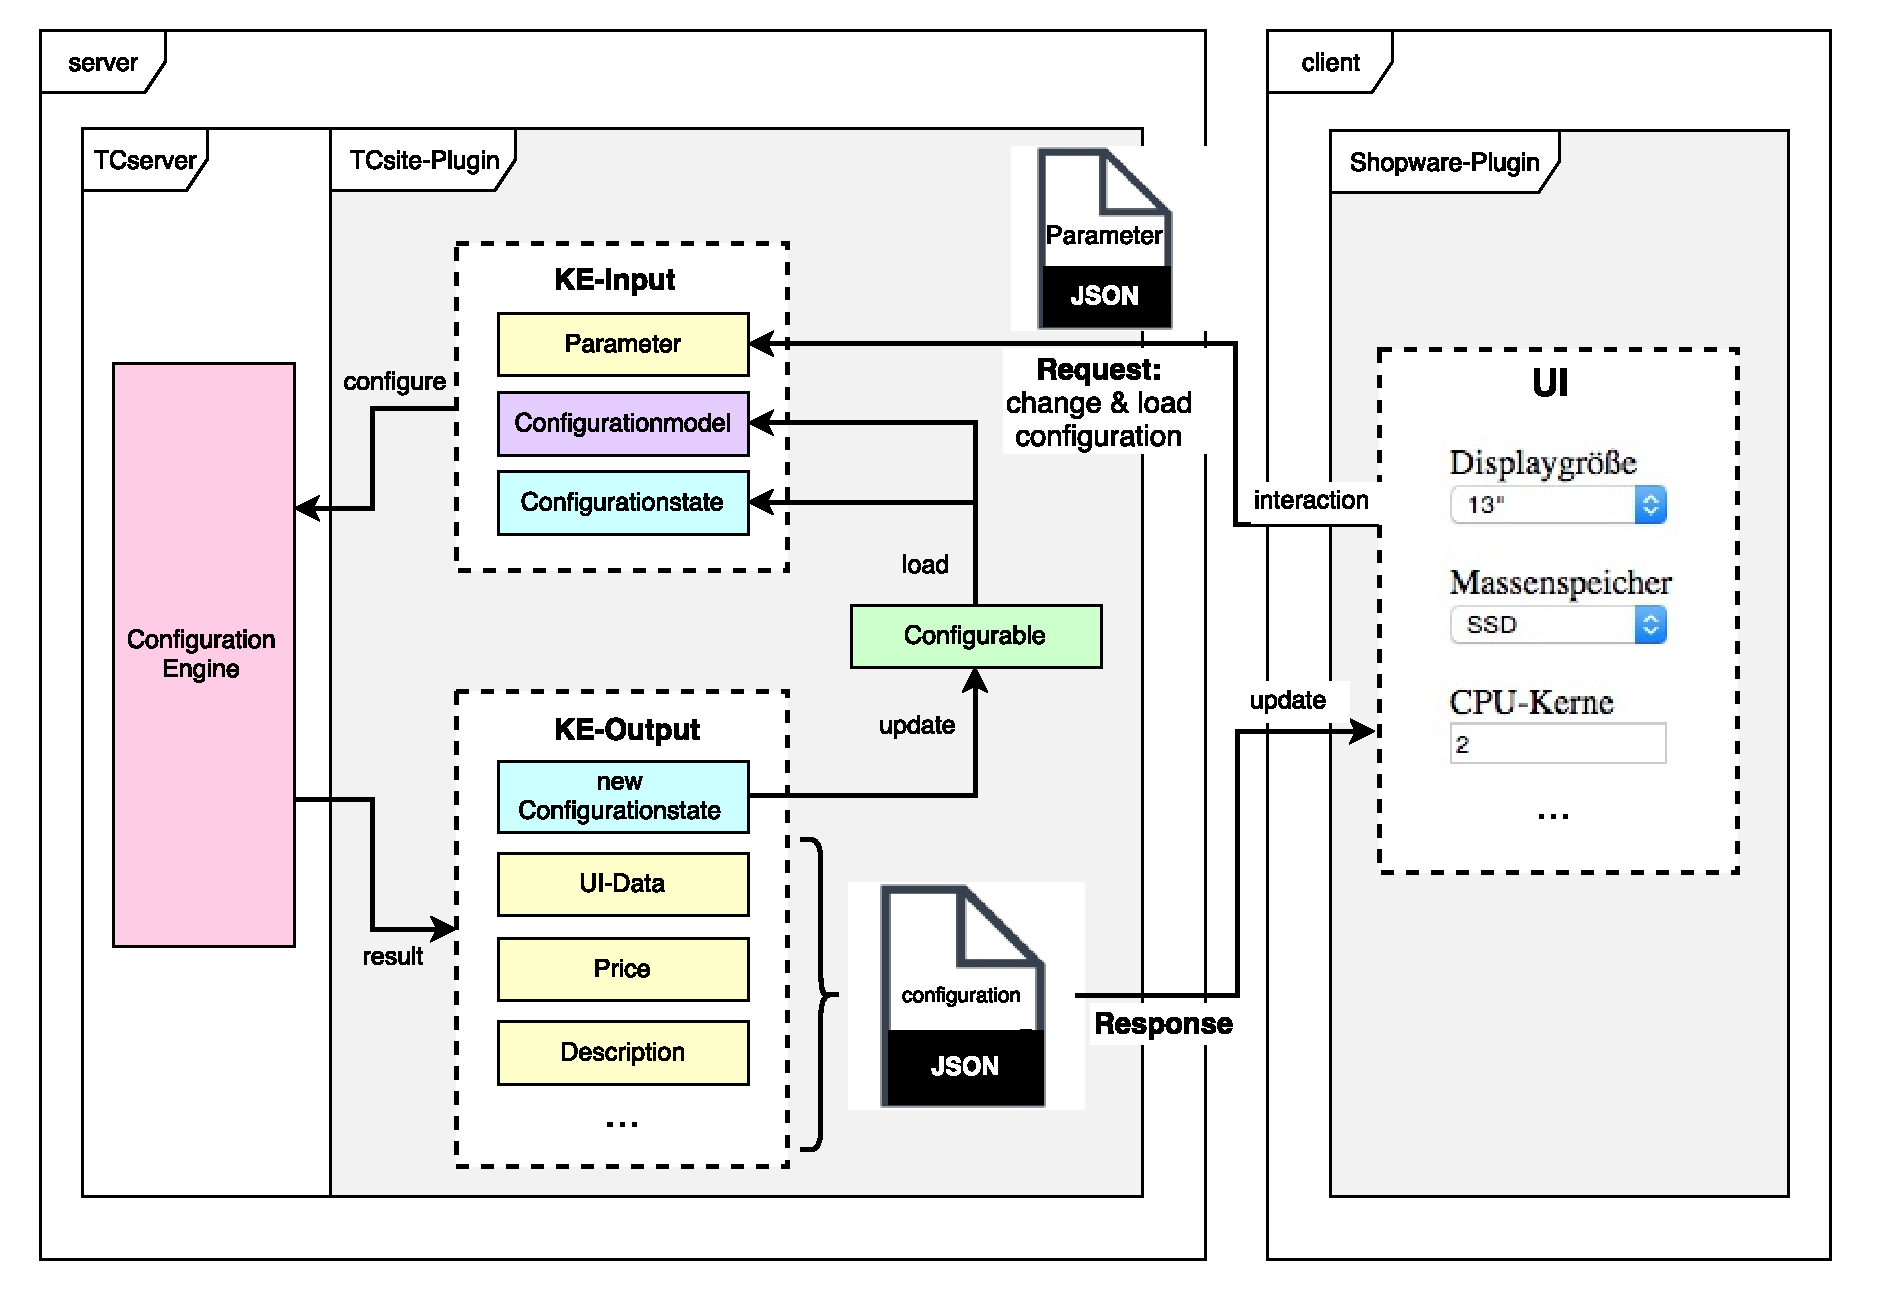
\includegraphics[width=1\linewidth]{Abbildungen/konzeptChange.pdf}
	\captionof{figure}[konzeptChange]{Ändern \& Laden einer \emph{configuration}-Ressource}
	\label{fig:konzeptChange}
\end{minipage}
\vspace{1em}

Nun klickt der Anwender den \glqq In den Warenkorb\grqq{}-Button, was im Falle einer neuen Konfiguration zum Anlegen einer Warenkorbposition führen soll. Standardmäßig wird durch den Button die \emph{ajaxAddArticleCart}-Action des Checkout-Controllers ausgelöst (die Controller-Terminologie wurde in Kapitel \ref{subsubsection:shopwareArchitektur} vorgestellt). In der Action wird die Warenkorbposition angelegt und der Warenkorb angezeigt. Die Besprechung des Datenbank-Relationenmodells (siehe Abbildung \ref{fig:shopwareArtikelRelationenModell} hat gezeigt, dass eine Warenkorbposition auf einen Variante verweist. Diese Variante existiert aber noch nicht, sondern muss noch dynamisch erzeugt werden. Die Analyse der Shopware-Erweiterbarkeit in Kapitel \ref{subsubsection:shopwareErweiterbarkeit} hat ergeben, dass Controller-Actions überschreibbar sind. \emph{ajaxAddArticleCart} wird also durch eine vom Shopware-Plugin bereitgestellt Funktion überschrieben.

Diese neue Funktion legt zunächst eine Variante an. Das heißt, sie erzeugt eine neue Zeile in der Tabelle \emph{s\_articles\_details}, siehe Abbildung \ref{fig:shopwareArtikelRelationenModell}. Für die Variante wird die entsprechende \emph{configurationID} in der Tabelle \emph{s\_articles\_details} hinterlegt. So ist die Variante mit der \emph{configuration}-Ressource verknüpft, durch die sie konfiguriert wurde. Der Preis der Variante wird in der Tabelle \emph{s\_articles\_details} hinterlegt.  Jetzt kann die entsprechende Warenkorbposition erzeugt werden. Der Name der Warenkorbposition wird nachträglich zu einer Kurzbeschreibung der Variante geändert (z.B. Notebook OSX Yosemite 4GB RAM). Die Kurzbeschreibung stammt ebenfalls aus der \emph{configuration}-Ressource. Zusammengefasst müssen der überschriebenen \emph{ajaxAddArticleCart}-Action drei zusätzliche Informationen übermittelt werden -- die \emph{configurationID}, der Preis und die Kurzbeschreibung.

\textbf{Warenkorb}\\
Die aktuelle Station des Einkaufsvorgangs ist der Warenkorb (siehe Abbildung \ref{fig:konzeptionEinkausvorgang1}). Möchte der Anwender weitere Artikel konfigurieren, schließt er den Warenkorb und beginnt mit der Auswahl der Wunschartikel. Damit wiederholt sich der bisher beschriebene Prozess. Ist der Anwender mit einer Warenkorbposition unzufrieden, kann er diese Löschen und Umkonfigurieren.

Im Gegensatz zum ursprünglichen Einkaufsvorgang (siehe Abbildung \ref{fig:shopwareKonfigurationFlussdiagramm}) hat das Löschen einer Warenkorbposition nun weitere Löschungen zur Folge. Eine Variante wurde nur erstellt, um als Bezugspunkt einer Warenkorbposition zu dienen. Das Löschen einer Position macht auch die zugehörige Variante obsolet. Dementsprechend wird diese aus der Datenbank entfernt. Durch die in Abbildung dargestellten \ref{fig:shopwareArtikelRelationenModell} Fremdschlüsselverweise werden in dessen Folge die entsprechenden Zeilen aus \emph{s\_articles\_prices} und \emph{s\_articles\_details} ebenfalls gelöscht. Auch die zugehörige \emph{configuration}-Ressource ist dadurch funktionslos. Ein Löschbefehl wird an das TCsite-Plugin abgesetzt.

Der standardmäßige Löschvorgang einer Warenkorbposition wird von der Methode \emph{sDeleteArticle} der Moduls \emph{sBasket} realisiert (siehe Abbildung \ref{fig:tcsiteLowLevel}). Es handelt sich nicht um eine Controller-Action und die Funktion enthält auch keine Notify-Events. Entsprechend der Erläuterung logischer Erweiterungen in Kapitel \ref{subsubsection:shopwareErweiterbarkeit} muss also auf das Hooksystem zurückgegriffen werden. Eine Plugin-Funktion wird der \emph{sDeleteArticle} \glqq angehangen\grqq{}, worin das Löschen der entsprechenden Variante und \emph{configuration} implementiert wir.

Die letzte Möglichkeit ist das Umkonfigurieren einer Warenkorbposition. Dies wird im Folgenden konzipiert.

\textbf{Umkonfiguration}\\
Durch einen Klick auf eine Warenkorbposition gelangt der Anwender zur Detailsansicht der Variante. Beim Anlegen der Variante wurde für diese eine \emph{configurationID} hinterlegt. Die zugehörige \emph{configuration} wird geladen, wodurch der letzte Stand der Konfigurationsoberfläche wieder hergestellt wird. Abbildung \ref{fig:konzeptCopy} zeigt den Vorgang im Detail.

Das Vorgehen entspricht insofern dem "Erstellen \& Laden einer neuen \emph{configuration}" (siehe Abbildung \ref{fig:konzeptCreate}), als dass der KE-Input ohne eine gewählte Option verarbeitet wird. Dementsprechend ist der Konfigurationszustand vor und nach dem Aufruf der Konfigurationsengine der selbe. Jedoch geschieht die Umkonfigurationsprozess auf einer Arbeitskopie und nicht auf dem \emph{configurable}, welches im Zusammenhang mit der \emph{configurationID} steht. Grund dafür ist Anforderung SW.F11. Gemäß dieser Anforderung muss die Umkonfiguration erst abschließend vom Anwender bestätigt werden. Es ist also möglich, dass der Anwender zunächst andere Optionen wählt, die Änderungen aber verwerfen möchte (z.B. in dem er die Detailseite ohne Bestätigung der Umkonfiguration verlässt). Ohne das Anfertigen einer Arbeitskopie würde im Falle des Verwerfens die \emph{configuration}-Ressource nicht mehr dem Konfigurationszustand entsprechen, mit dem mit die Variante in Shopware ursprünglich angelegt wurde.

\vspace{1em}
\begin{minipage}{\linewidth}
	\centering
	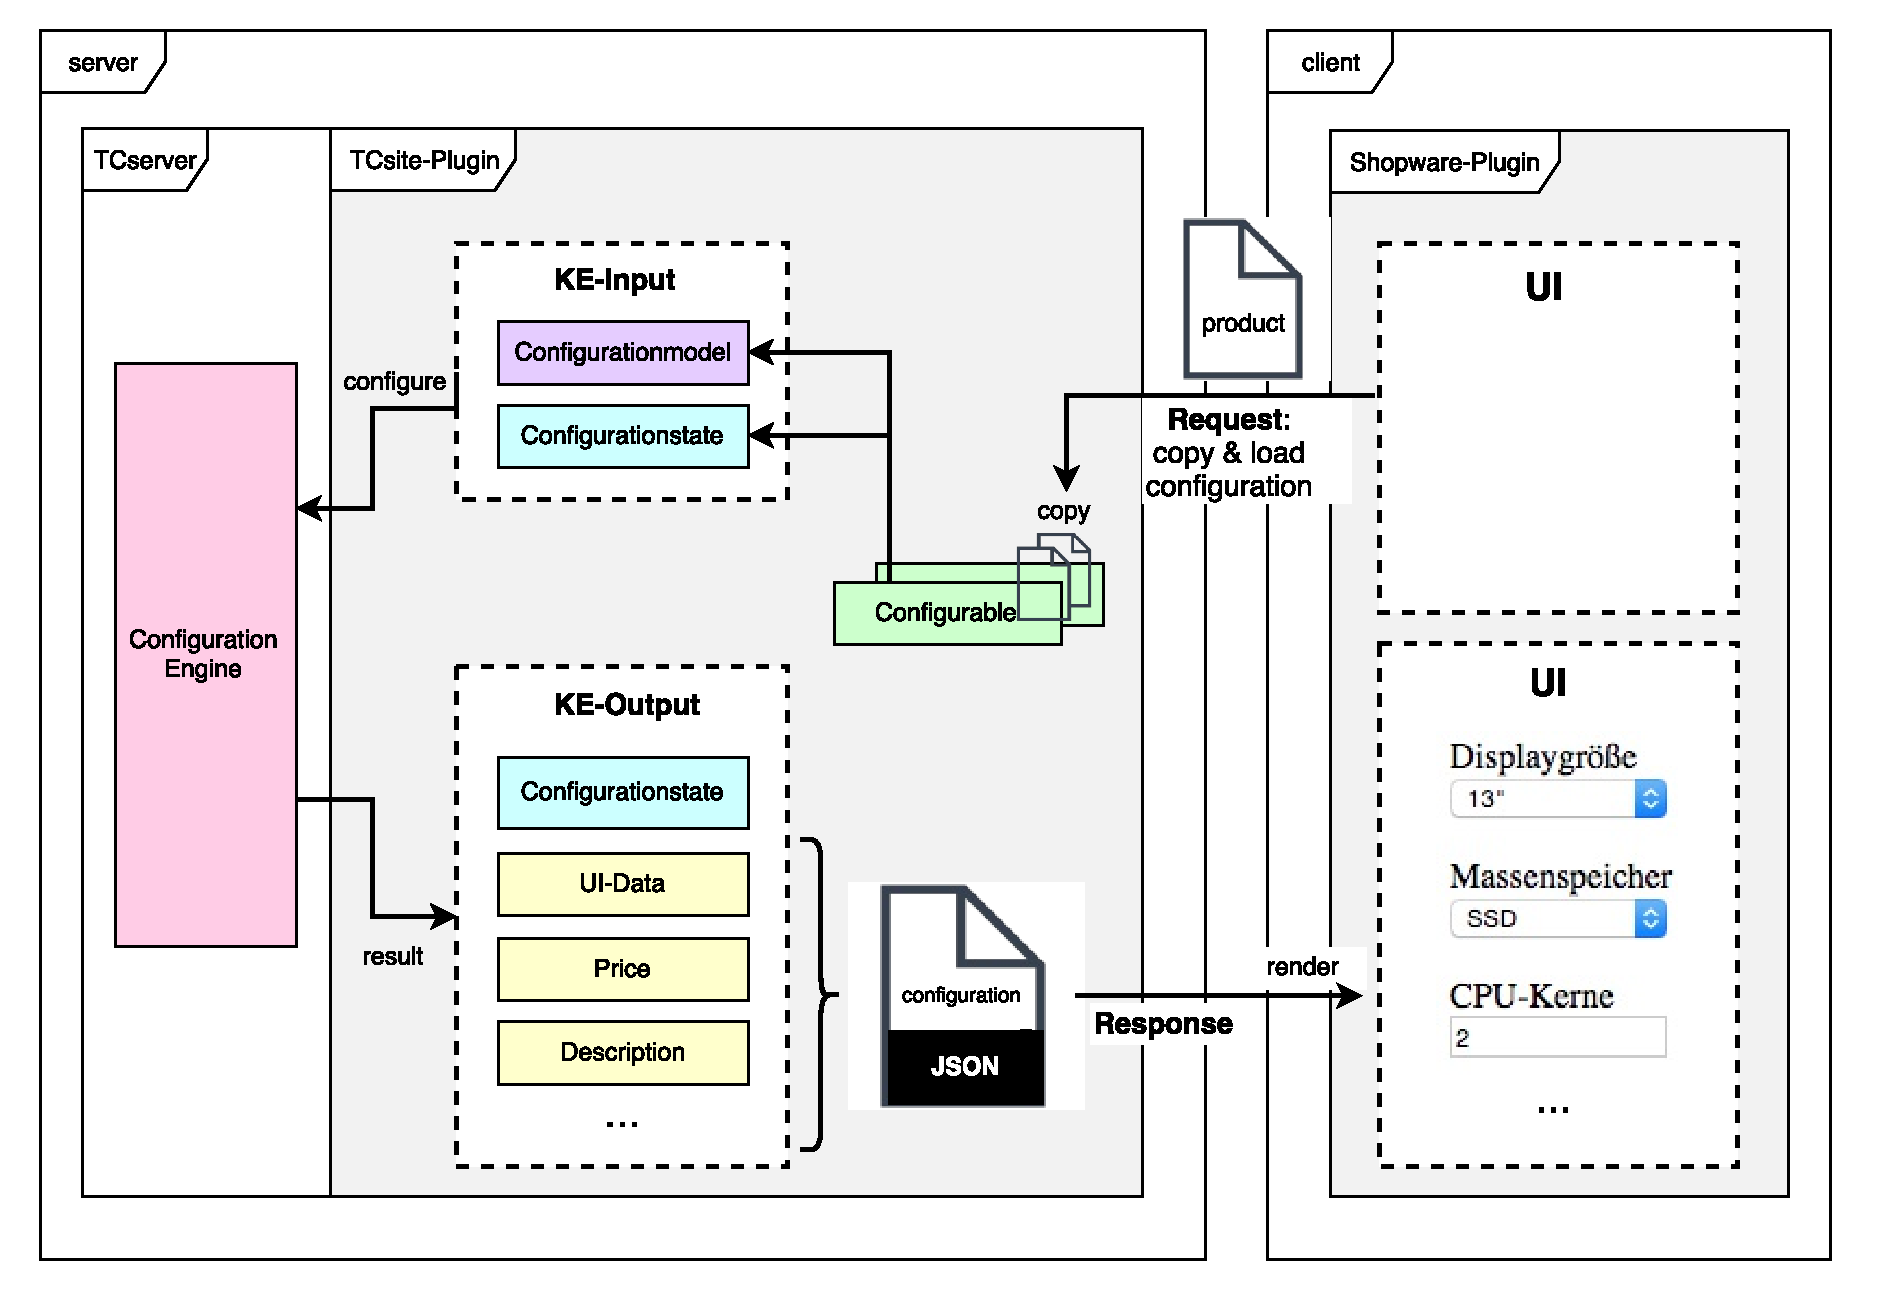
\includegraphics[width=1\linewidth]{Abbildungen/konzeptCopy.pdf}
	\captionof{figure}[konzeptCopy]{Kopieren \& Laden einer bestehenden \emph{configuration}}
	\label{fig:konzeptCopy}
\end{minipage}
\vspace{1em}

Die Beschriftung des \glqq In den Warenkorb\grqq{}-Buttons muss auf \glqq Neue Konfiguration Speichern\grqq geändert werden. So wird darauf Hingewiesen, dass das Verhalten des Buttons ein anderes ist. Inwiefern, wird im Folgenden beschrieben.

Die entsprechende Warenkorbposition muss nicht inkrementiert (entspricht dem Verhalten aus Abbildung \ref{subsubsection:shopwareKonfiguration}), sondern aktualisiert werden. Das Betrifft den Preis (Spalte: \emph{price}; Tabelle \emph{s\_articles\_prices}), die Beschreibung (Spalte: \emph{articlename}; Tabelle \emph{s\_order\_basket}) und die Anzahl (Spalte: \emph{quantity}; Tabelle \emph{s\_order\_basket}). Außerdem muss die \emph{configurationID} dieser Variante aktualisiert werden, da die Änderungen auf einer Arbeitskopie stattfanden.

Zur Implementierung des neuen Verhalten wird die bereits überschriebene \emph{ajaxAddArticleCart}-Action genutzt. Zwar wurde die Beschriftung des \glqq In den Warenkorb\grqq{}-Buttons geändert, er triggert aber immer noch die gleiche Controllerfunktion. In der überschriebenen Action muss Unterschieden werden, ob es sich um eine neue Konfiguration oder eine Umkonfiguration handelt. Letzteres in dann der Fall, wenn für die Variante bereits eine \emph{configurationID} hinterlegt ist.

\textbf{Bestellung}\\
Die Erstellten Varianten gehen als normale Artikel in den Bestellprozess ein. Im Eingang dieses Kapitels wurde erwähnt, dass über die \emph{ordnernumber} einer Variante (Tabelle \emph{s\_articles\_details}) die bestellte Warenkorbposition vom Vertrieb zugeordnet werden kann. Die Varianten wurden im eben dargestellten Ablauf jedoch automatisiert während Einkaufsvorgang generiert. Die \emph{ordernumber} gibt also keine Auskunft über die vorliegende Variante. Entweder ist die Beschreibung der Variante aussagekräftig genug, oder die \emph{configurationID} ermöglicht die Auswertung der Daten, die bei TCsite mit dieser Bestellung im Zusammenhang stehen. Genaueres zur letzteren Vorgehensweise wird in der Konzeption des TCsite-Plugins besprochen.

\subsubsection{Zusammenfassung}
Vorausgehend wurden alle notwendigen Erweiterungen des Shopware-Plugins beschrieben und begründet, wobei der Einkaufsvorgang in Abbildung \ref{fig:konzeptionEinkausvorgang1}
 als Strukturierungsvorlage der Darstellung diente. Im Folgenden werden die notwendigen Erweiterungen nach Typen zusammengefasst:
 
\begin{enumerate}
\item \textbf{Daten-Erweiterungen:}
\begin{enumerate}[(a)]
\item Hinzufügen von Variantenattributen\\
Spalten: \emph{correspondingTcsiteProduct} / \emph{configurationID}, Tabelle \emph{s\_articles\_details}
\end{enumerate}
\item \textbf{Template-Erweiterungen:}
\begin{enumerate}[(a)]
\item Ersetzen des Preises im Artikellisting\\Smarty-Block: \emph{frontend\_listing\_box\_article\_price\_default}
\item Einfügen der Konfigurationsoberfläche in der Detailseite\\Smarty-Block: \emph{frontend\_detail\_index\_detail}
\item Einfügen von clientseitiger Logik mittels Einbindung von Javascript-Dateien in der Detailseite\\Smarty-Block: \emph{frontend\_index\_header\_javascript}
\item Einfügen eines Textfeldes im Artikelmenü des Backends zur Eingabe des korrespondierenden TCsite-Produkts\\Block: \emph{frontend\_index\_header\_javascript}
\end{enumerate}
\item \textbf{logische Erweiterungen:}
\begin{enumerate}[(a)]
\item Überschreiben der Controller-Action zum Hinzufügen von Warenkorbpositionen\\
Action: \emph{ajaxAddArticleCart}, Controller: \emph{Checkout}
\item \glqq Hooken\grqq{} der Methode zum Löschen von Warenkorbartikeln\\
Methode: \emph{sDeleteArticle}, Modul: \emph{sBasket}
\end{enumerate}
\end{enumerate}

\subsection{anker}





\newpage
\begin{table}[]
\centering
\caption{My caption}
\label{my-label}
\begin{tabularx}{\textwidth}{|X|X|X|X|X|X|}
\hline
\multirow{2}{*}{{\bf Methode}} & \multirow{2}{*}{{\bf Bechreibung}} & \multicolumn{1}{l|}{{\bf Parameter}} & \multicolumn{1}{l|}{} & \multicolumn{1}{l|}{} &                                                                                                                           \\ \cline{3-6} 
                               &                                    & {\bf id}                             & {\bf product}         & {\bf operation}       & \multicolumn{1}{c|}{{\bf \begin{tabular}[c]{@{}c@{}}action,\\ parameter,\\ value,\\ currentGroup,\\ accept\end{tabular}}} \\ \hline
{\bf GET}                      & conf. holen                & x                                    &                       & \multicolumn{1}{l|}{} &                                                                                                                           \\ \hline
{\bf DELETE}                   & conf. löschen              & x                                    &                       & \multicolumn{1}{l|}{} &                                                                                                                           \\ \hline
{\bf POST}                     & conf. erstellen            &                                      & x                     & create                &                                                                                                                           \\ \hline
                               & conf. kopieren             & x                                    &                       & copy                  &                                                                                                                           \\ \hline
                               & conf. verändern            & x                                    &                       & change                & \multicolumn{1}{c|}{x}                                                                                                    \\ \hline
\end{tabularx}
\end{table}

\pagebreak

\section{Umsetzung}

\pagebreak

\section{Fazit}

\pagebreak

% ----------------------------------------------------------------------------------------------------------
% Literatur
% ----------------------------------------------------------------------------------------------------------
\renewcommand\refname{Quellenverzeichnis}
\bibliographystyle{myalpha}
\bibliography{bibo}
\pagebreak

% ----------------------------------------------------------------------------------------------------------
% Anhang
% ----------------------------------------------------------------------------------------------------------

\renewcommand\refname{Anhang}
\begin{appendix}
\chapter{Anhang}

\vspace{1em}
\begin{minipage}{\linewidth}
	\centering
	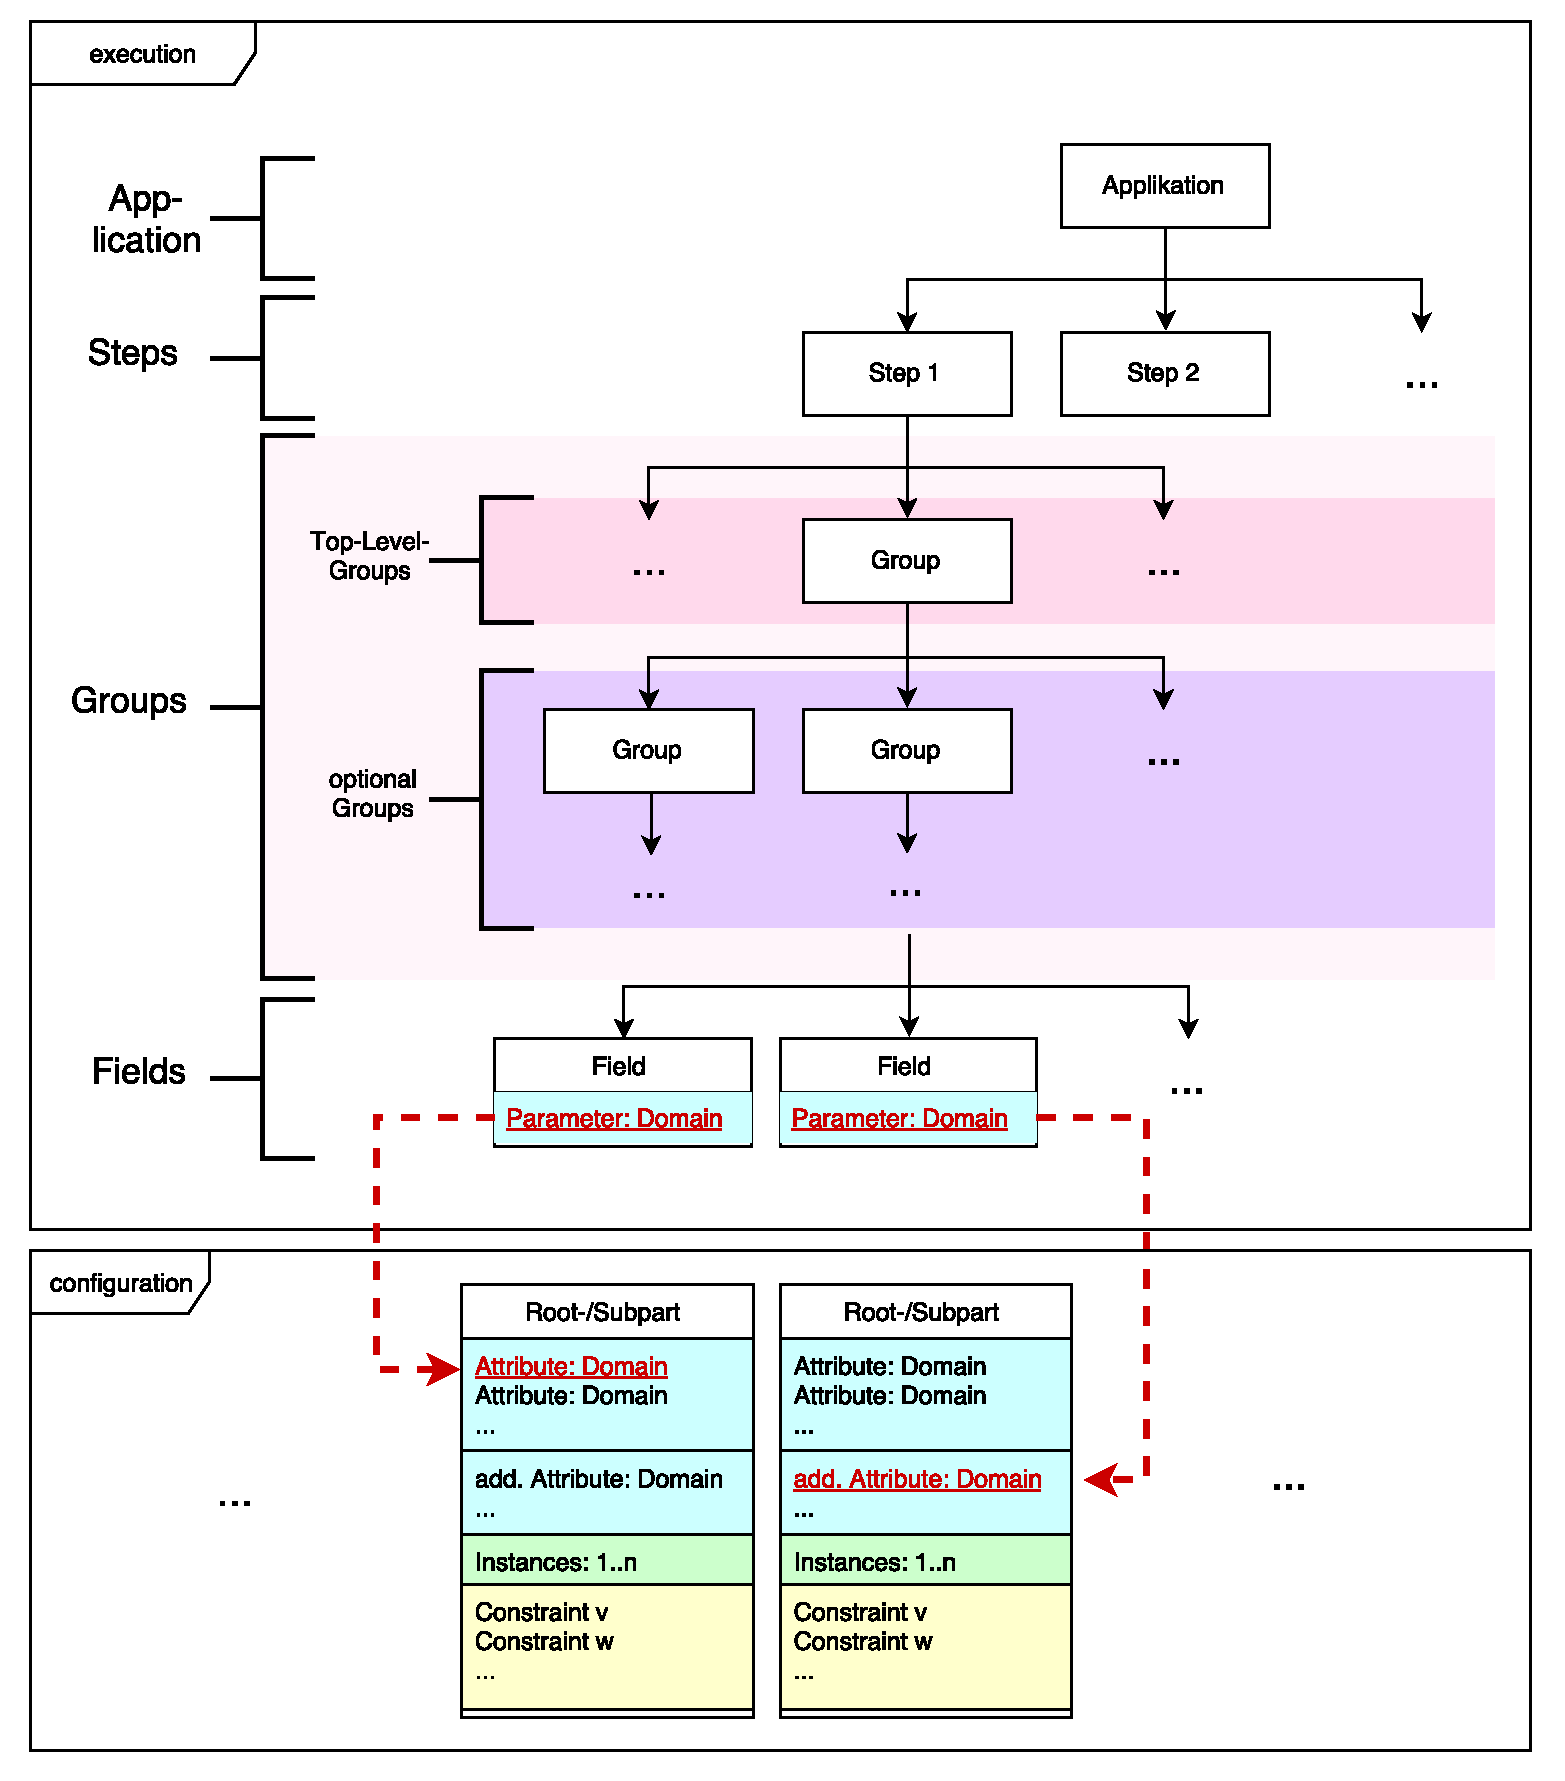
\includegraphics[width=1\linewidth]{Abbildungen/tactonModellExecution.pdf}
	\captionof{figure}[Vollständige Darstellung der generischen Execution-Struktur]{Vollständige Darstellung der generischen Execution-Struktur}
	\label{app:tactonModellExecutionLong}
\end{minipage}
\vspace{1em}

\vspace{1em}
\begin{minipage}{\linewidth}
	\centering
	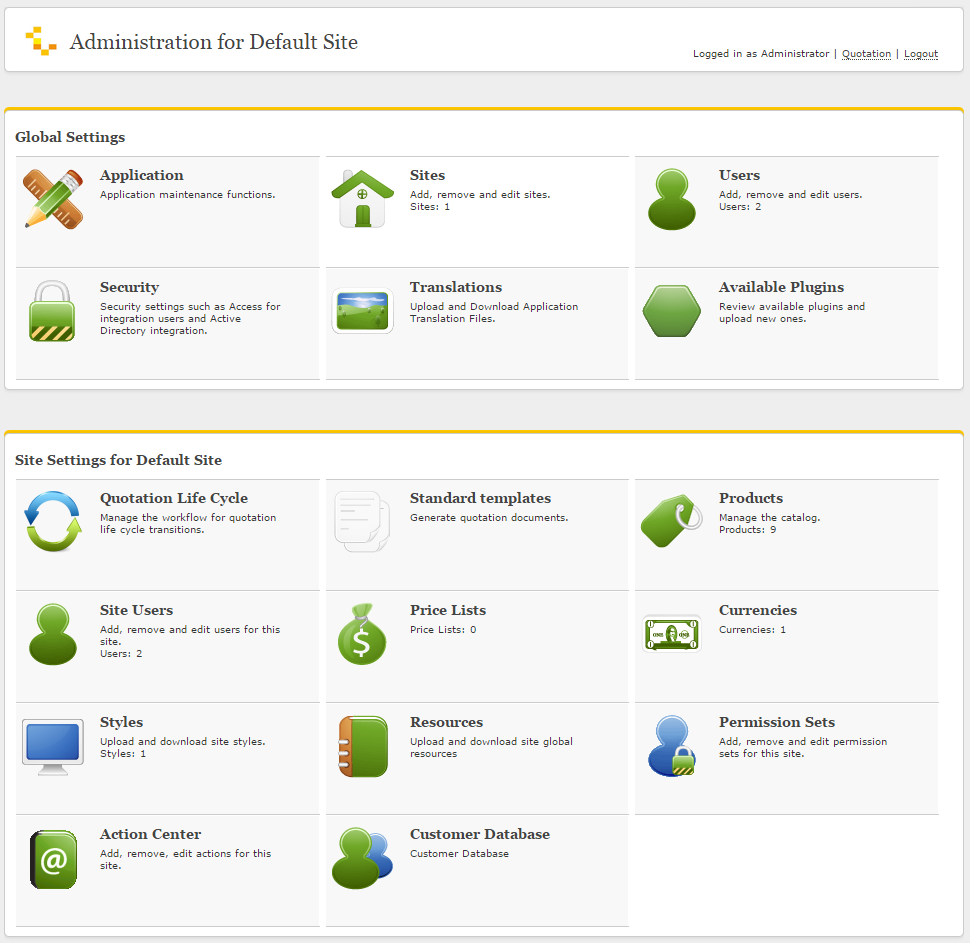
\includegraphics[width=1\linewidth]{Abbildungen/tcsiteAdministration.PNG}
	\captionof{figure}[tcsiteAdministration]{TCsite Administrationsoberfläche}
	\label{app:tcsiteAdministration}
\end{minipage}
\vspace{1em}

\vspace{1em}
\begin{minipage}{\linewidth}
	\centering
	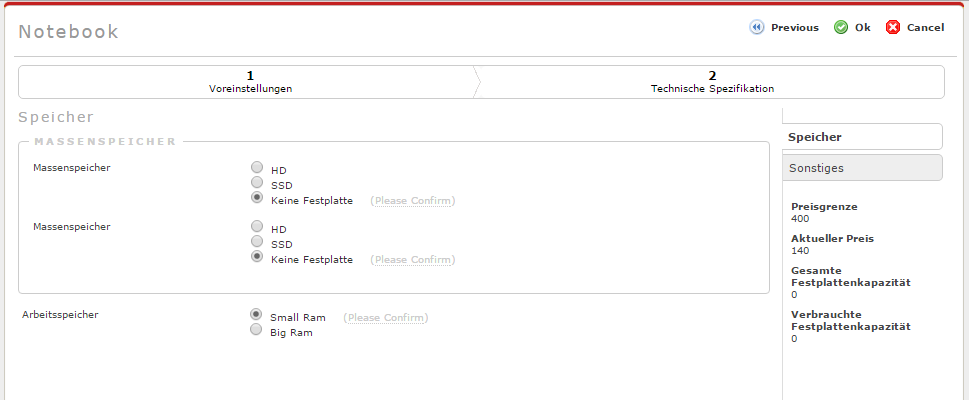
\includegraphics[width=1\linewidth]{Abbildungen/tcSiteConfigurationOptionalGroups.PNG}
	\captionof{figure}[tcSiteConfigurationOptionalGroups]{Darstellung optionaler Groups in TCsite}
	\label{app:tcSiteConfigurationOptionalGroups}
\end{minipage}
\vspace{1em}

\vspace{1em}
\begin{minipage}{\linewidth}
	\centering
	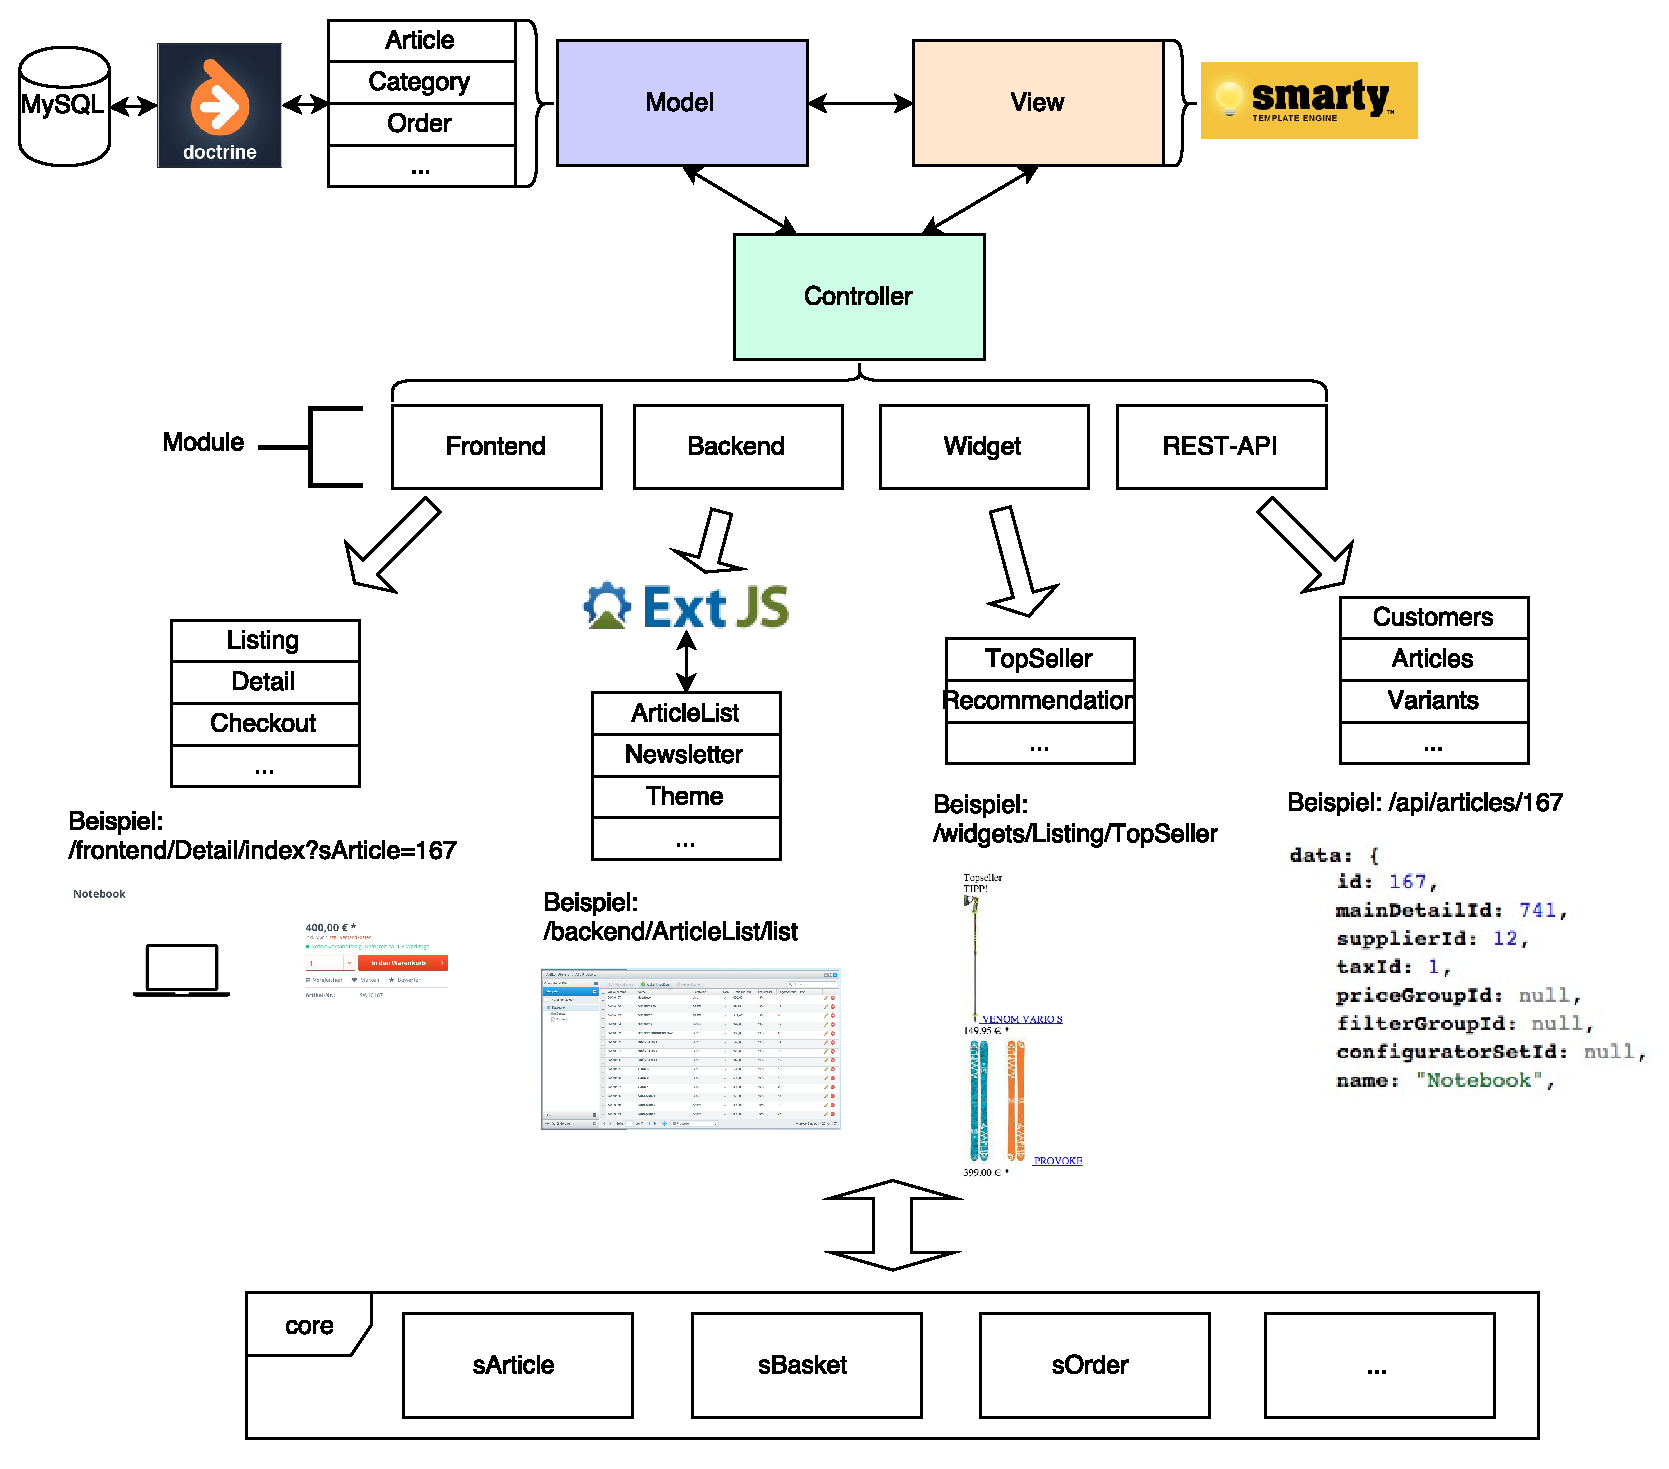
\includegraphics[width=1\linewidth]{Abbildungen/shopwareMVC.pdf}
	\captionof{figure}[vollständige High-Level-Architektur von Shopware]{vollständige Shopware High-Level-Architektur}
	\label{fig:shopwareMVCLong}
\end{minipage}
\vspace{1em}

\vspace{1em}
\begin{minipage}{\linewidth}
	\centering
	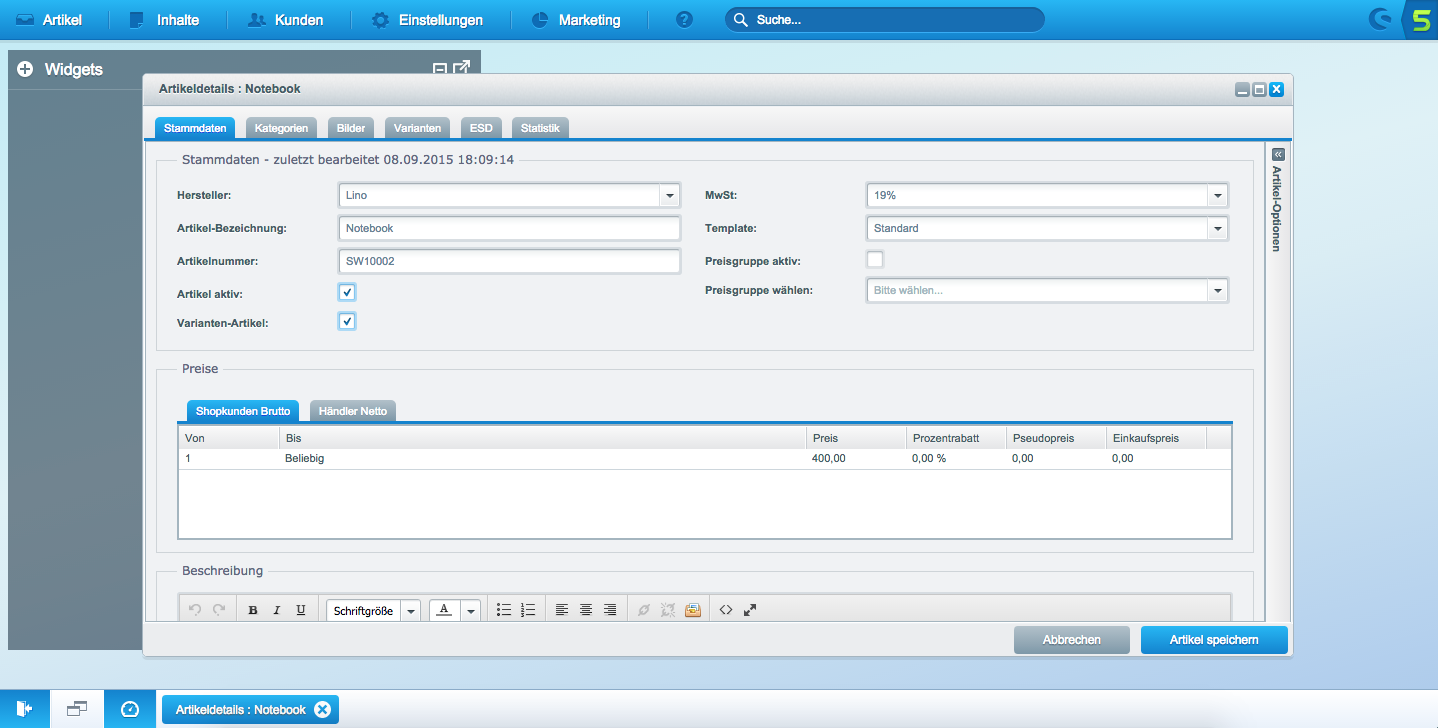
\includegraphics[width=1\linewidth]{Abbildungen/shopwareBackendArtikel.png}
	\captionof{figure}[shopwareBackendArtikel]{Anlegen eines Artikels im Backend}
	\label{app:shopwareBackendArtikel}
\end{minipage}
\vspace{1em}

\vspace{1em}
\begin{minipage}{\linewidth}
	\centering
	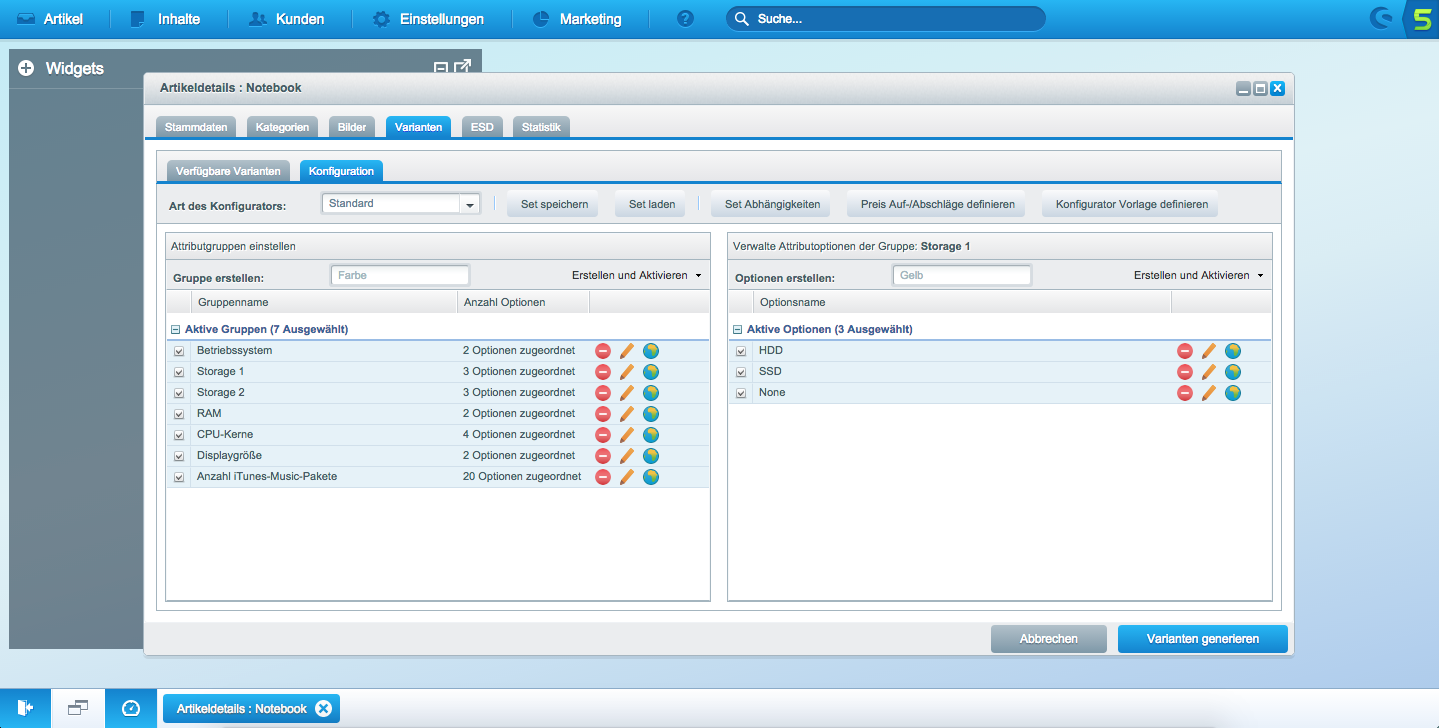
\includegraphics[width=1\linewidth]{Abbildungen/shopwareBackendArtikelVarianten.png}
	\captionof{figure}[shopwareBackendArtikelVarianten]{Generieren der Varianten im Backend}
	\label{app:shopwareBackendArtikelVarianten}
\end{minipage}
\vspace{1em}

\vspace{1em}
\begin{minipage}{\linewidth}
	\centering
	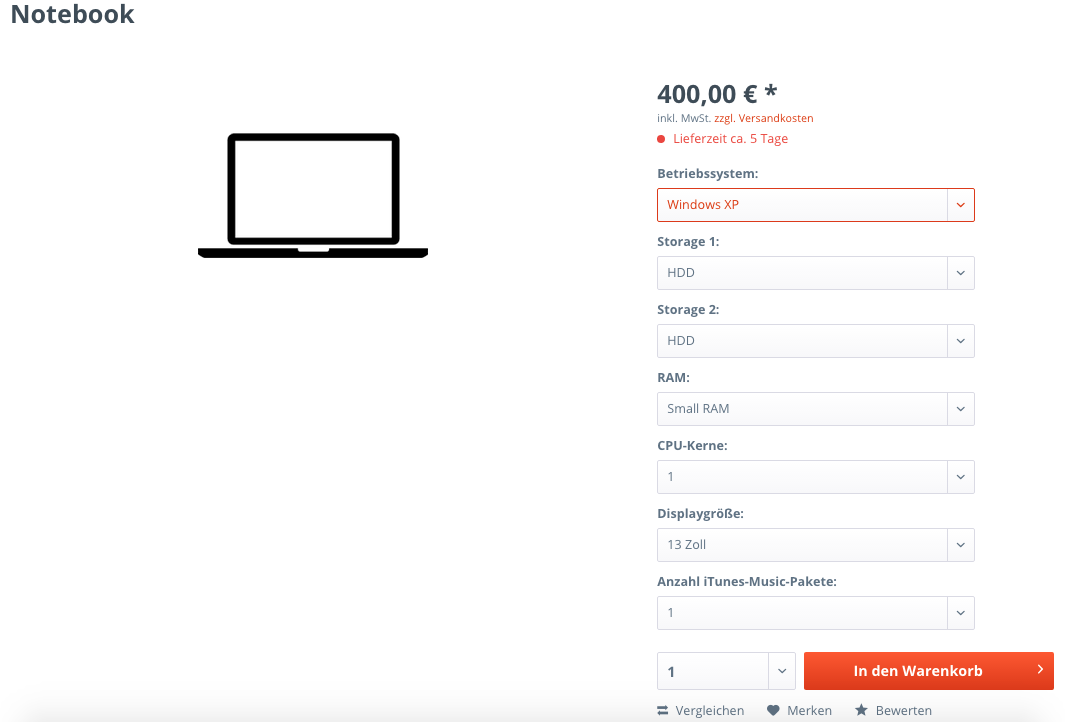
\includegraphics[width=1\linewidth]{Abbildungen/shopwareNotebookDetail.png}
	\captionof{figure}[shopwareNotebookDetail]{Detailansicht eines konfigurierbaren Notebooks in shopware.}
	\label{app:shopwareNotebookDetail}
\end{minipage}
\vspace{1em}

\vspace{1em}
\begin{minipage}{\linewidth}
	\centering
	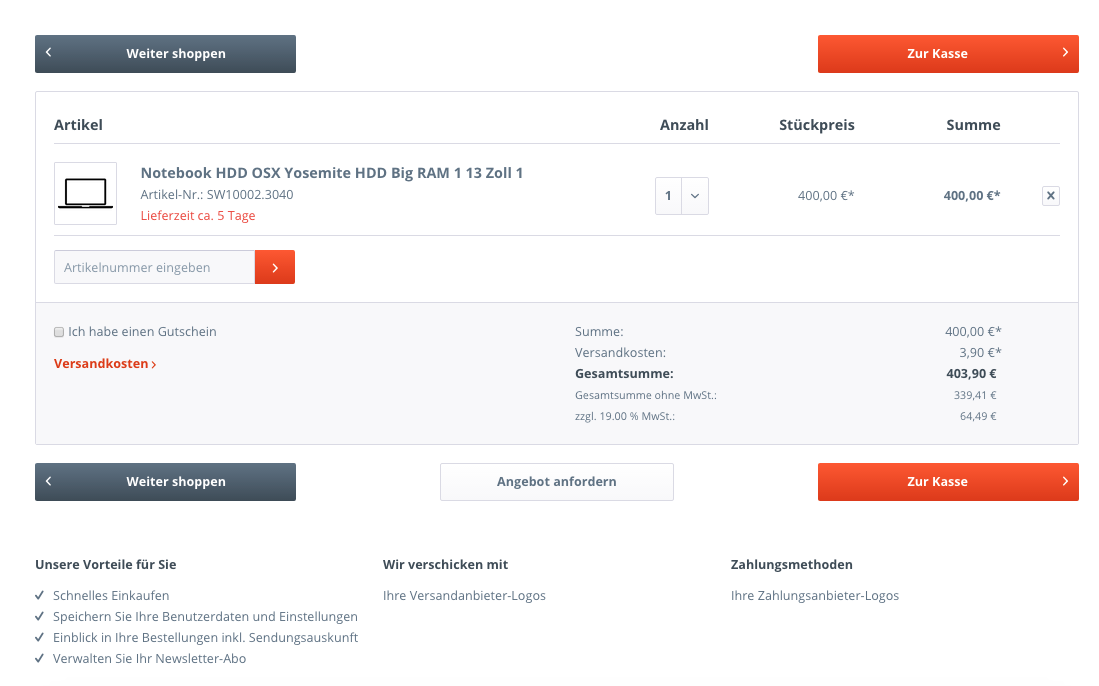
\includegraphics[width=1\linewidth]{Abbildungen/shopwareNotebookWarenkorb.png}
	\captionof{figure}[shopwareNotebookWarenkorb]{Warenkorb mit konfiguriertem Artikel.}
	\label{app:shopwareNotebookWarenkorb}
\end{minipage}
\vspace{1em}

\vspace{1em}
\begin{minipage}{\linewidth}
	\centering
	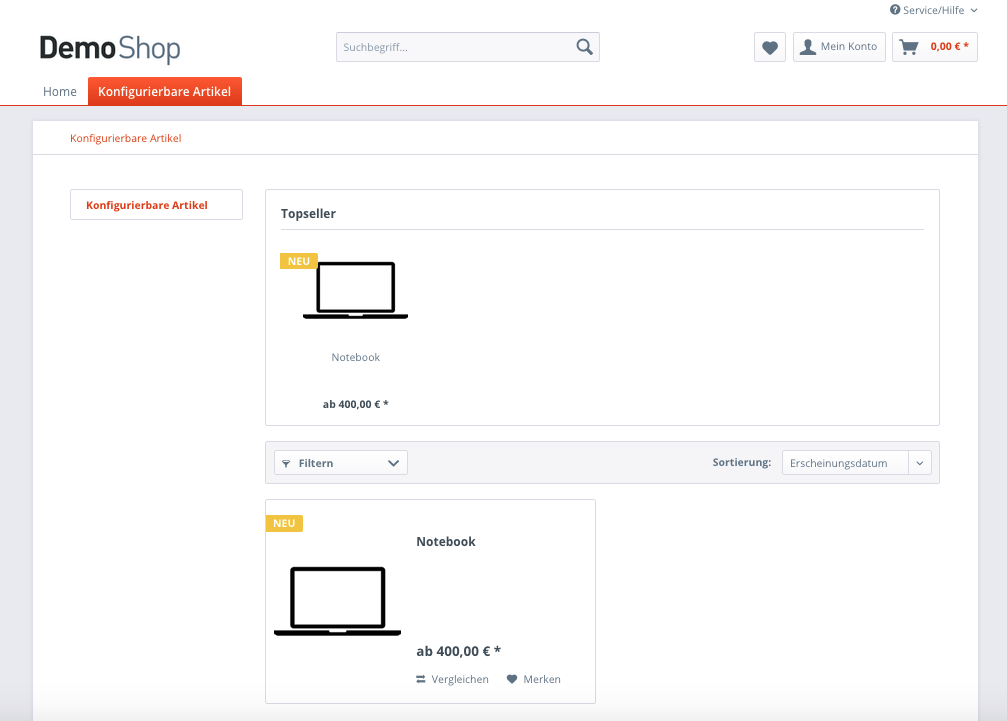
\includegraphics[width=1\linewidth]{Abbildungen/shopwareArtikelListing.png}
	\captionof{figure}[Artikellisting in Shopware]{Artikellisting in Shopware}
	\label{app:shopwareArtikelListing}
\end{minipage}
\vspace{1em}

\vspace{1em}
\begin{minipage}{\linewidth}
	\centering
	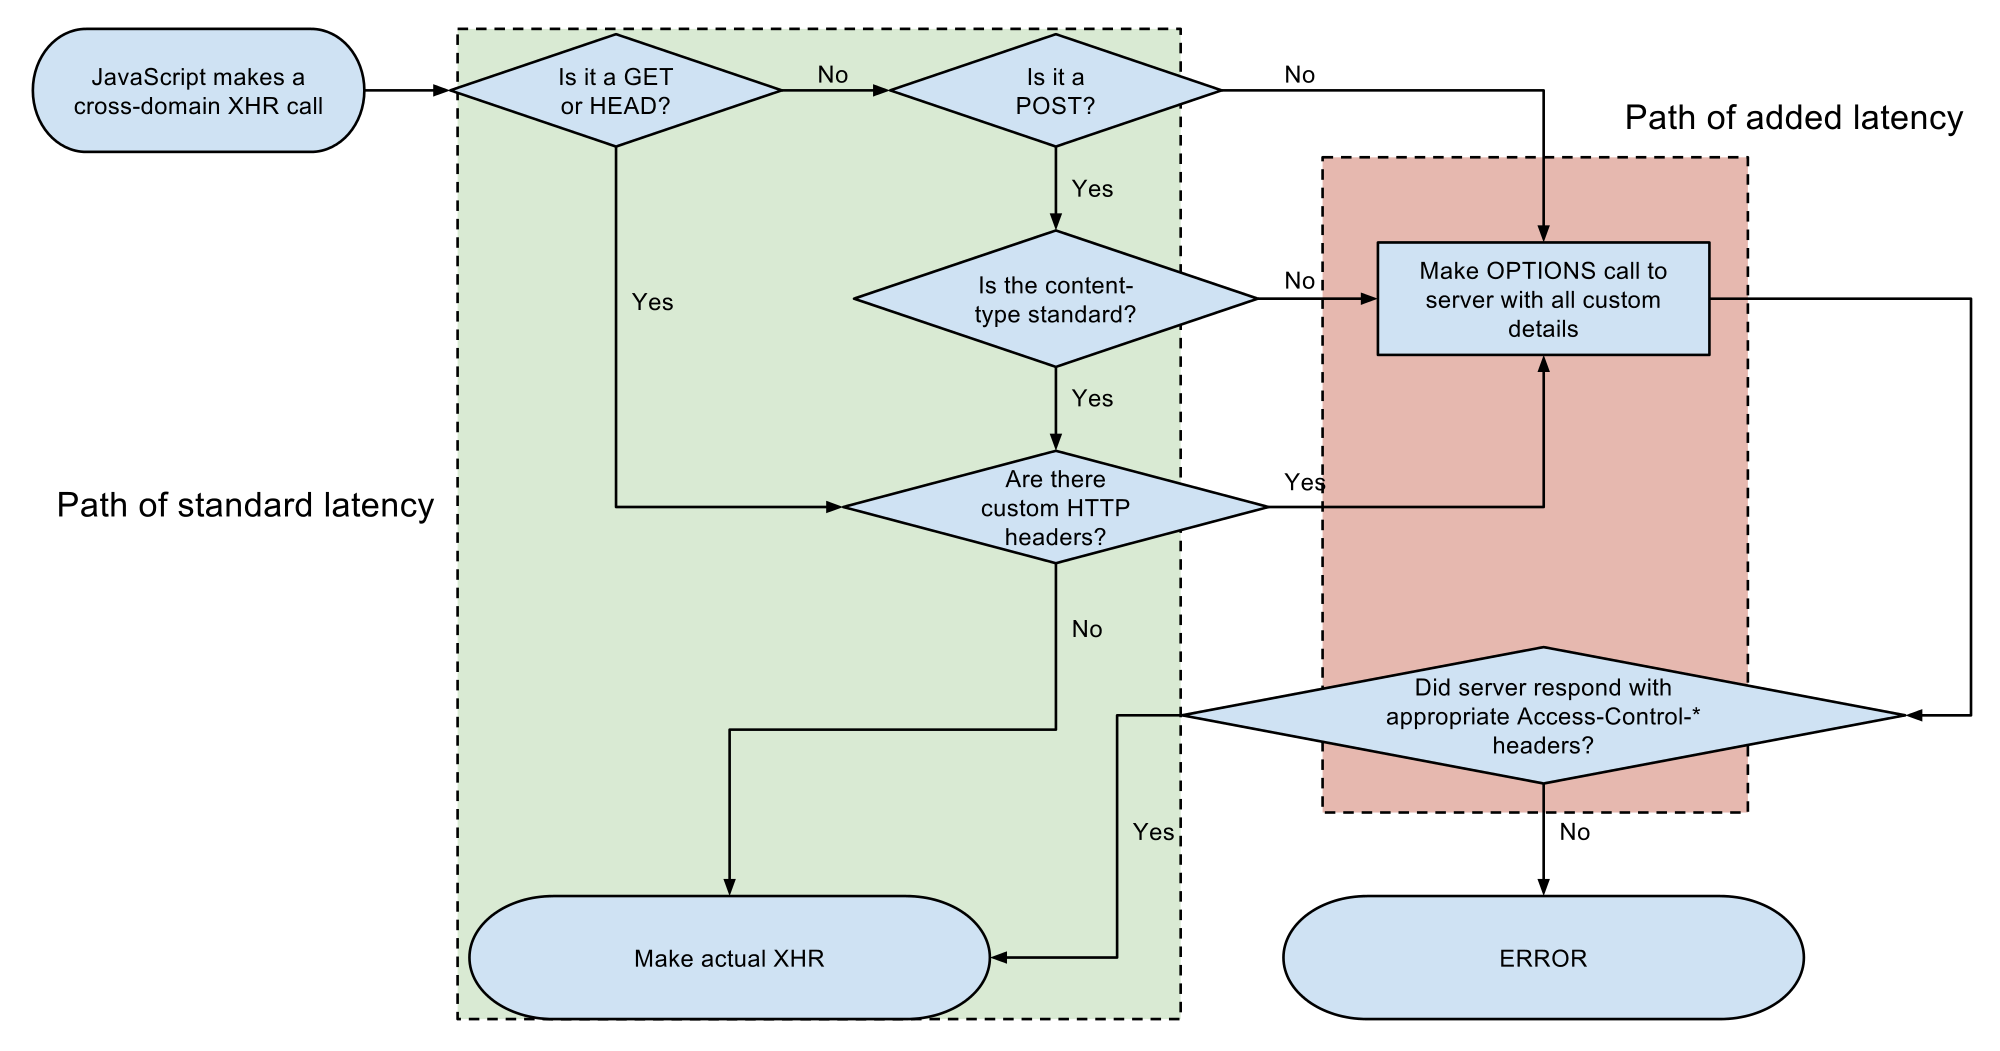
\includegraphics[width=1\linewidth]{Abbildungen/mozillaCORS.png}
	\captionof{figure}[mozillaCORS]{CORS-Flowchart.}
	\label{app:mozillaCORS}
\end{minipage}
\vspace{1em}

\end{appendix}

\chapter*{Selbstständigkeitserklärung}
\vspace{2em}
Ich versichere hiermit an Eides statt, dass ich die vorliegende Bachelorarbeit selbstständig und ohne unzulässige fremde Hilfe erbracht habe. Ich habe keine anderen als die angegebenen Quellen und Hilfsmittel benutzt sowie wörtliche und sinngemäße Zitate kenntlich gemacht. Die Arbeit hat in gleicher oder ähnlicher Form noch keiner Prüfungsbehörde
vorgelegen.

\vspace{4em}
\begin{minipage}{\linewidth}
	\begin{tabular}{p{15em}p{15em}}
		Datum: &  .......................................................\\
		& \centering (Unterschrift)\\
	\end{tabular}
\end{minipage}

\end{document}
